\documentclass{book}
\usepackage{amsmath,amssymb}
\usepackage{graphicx}
\usepackage{hyperref}

% plasTeX-only stubs (real packages dropped: mathtools, euscript, amsrefs)
\providecommand{\xRightarrow}[1]{\Rightarrow}
\providecommand{\coloneqq}{\mathrel{:=}}
\providecommand{\mathscr}[1]{\mathcal{#1}}

\theoremstyle{plain}
%!TEX root = TQFTnotes.tex
%%%%%%%  Theorems etc
\newtheorem{theorem}{Theorem}[section]
\newtheorem{proposition}[theorem]{Proposition}
\newtheorem{lemma}[theorem]{Lemma}
\newtheorem{corollary}[theorem]{Corollary}
\newtheorem{conjecture}[theorem]{Conjecture}
%%%%%%
\theoremstyle{definition}
\newtheorem{definition}{Definition}[section]
\newtheorem{predefinition}[theorem]{Preliminary Definition}
\newtheorem{remark}{Remark}[section]
\newtheorem{convention}{Convention}[section]
\newtheorem{example}{Example}[section]
%\newtheorem{problem}[theorem]{Problem}
\newtheorem{exercise}{Exercise}[section]
\newtheorem{examples}[example]{Examples}


%%%%%%%% References to ...
\newcommand{\chref}[1]{\hyperref[#1]{Chapter~{\rm\ref*{#1}}}}
\newcommand{\seref}[1]{\hyperref[#1]{Section~{\rm\ref*{#1}}}}
\newcommand{\firef}[1]{\hyperref[#1]{Figure~{\rm\ref*{#1}}}}
\newcommand{\thref}[1]{\hyperref[#1]{Theorem~{\rm\ref*{#1}}}}
\newcommand{\prref}[1]{\hyperref[#1]{Proposition~{\rm\ref*{#1}}}}
\newcommand{\leref}[1]{\hyperref[#1]{Lemma~{\rm\ref*{#1}}}}
\newcommand{\coref}[1]{\hyperref[#1]{Corollary~{\rm\ref*{#1}}}}
\newcommand{\deref}[1]{\hyperref[#1]{Definition~{\rm\ref*{#1}}}}
\newcommand{\exref}[1]{\hyperref[#1]{Example~{\rm\ref*{#1}}}}
\newcommand{\ecref}[1]{\hyperref[#1]{Exercise~{\rm\ref*{#1}}}}
\newcommand{\reref}[1]{\hyperref[#1]{Remark~{\rm\ref*{#1}}}}

%%%%%%%%% Greek letters
\newcommand{\al}{\alpha}
\newcommand{\be}{\beta}
\newcommand{\ga}{\gamma}
\newcommand{\Ga}{\Gamma}
\newcommand{\de}{\delta}
\newcommand{\De}{\Delta}
\newcommand{\eps}{\varepsilon}
\newcommand{\la}{\lambda}
\newcommand{\ph}{\varphi}
\newcommand{\Si}{\Sigma}
\newcommand{\si}{\sigma}
\newcommand{\om}{\omega}

%%%%%%%%% calligraphic letters
\newcommand{\calA}{\mathcal{A}}
\newcommand{\calB}{\mathcal{B}}
\newcommand{\calC}{\mathcal{C}}
\newcommand{\calD}{\mathcal{D}}
\newcommand{\calE}{\mathcal{E}}
\newcommand{\calF}{\mathcal{F}}
\newcommand{\calH}{\mathcal{H}}
\newcommand{\calK}{\mathcal{K}}
\newcommand{\calL}{\mathcal{L}}
\newcommand{\calM}{\mathcal{M}}
\newcommand{\calN}{\mathcal{N}}
\newcommand{\calZ}{\mathcal{Z}}
\newcommand{\calW}{\mathcal{W}}
%%%%%%%% fields
\newcommand{\Z}{\mathbb{Z}}
\newcommand{\R}{\mathbb{R}}
\newcommand{\C}{\mathbb{C}}
\newcommand{\kk}{\mathbf{k}}
\newcommand{\dd}{\mathbf{d}}
%%%%%%%% Lie groups and algebras
\newcommand{\SO}{\mathrm{SO}}
\newcommand{\OO}{\mathrm{O}}
\newcommand{\SU}{\mathrm{SU}}
\newcommand{\su}{\mathfrak{su}}
\newcommand{\GL}{\mathrm{GL}}
\newcommand{\g}{\mathfrak{g}}
%%%%%%%%%%%% categories
\newcommand{\Top}{\mathbf{Top}}
\newcommand{\Tam}{\mathbf{Tam}}
\newcommand{\Seg}{\mathbf{Seg}}
\newcommand{\sets}{\mathbf{Set}}
\newcommand{\ssets}{\mathbf{sSet}}
\newcommand{\svect}{\mathbf{SVec}}
\newcommand{\vect}{\mathbf{Vec}}
\newcommand{\vecf}{\mathbf{Vec_f}}
\newcommand{\cat}{\mathbf{Cat}}
\newcommand{\ab}{\mathbf{Ab}}
\newcommand{\abf}{\mathbf{Ab_f}}
\newcommand{\smoothman}{\mathbf{Man}}
\newcommand{\plman}{\mathbf{PLMan}}
\newcommand{\nCob}{\mathbf{Cob}_n}
\newcommand{\oneCob}{\mathbf{Cob}_1}
\newcommand{\twoCob}{\mathbf{Cob}_2}
\newcommand{\Bord}{\mathbf{Bord}}
\newcommand{\Bordfr}{\mathbf{Bord^{fr}}}
\newcommand{\Bordor}{\mathbf{Bord^{or}}}
\newcommand{\cfd}{\widetilde{\calC^{\fd}}}
\newcommand{\Linlf}{\mathbf{Lin}}
\newcommand{\Linf}{\mathbf{Lin_f}}
\newcommand{\Alg}{\mathbf{Alg}}
\newcommand{\ssAlg}{\mathbf{ssAlg}}
\newcommand{\ssfrob}{\mathbf{ssFrob}}
\newcommand{\Tens}{\mathbf{Tens}}
\renewcommand{\mod}{\mathbf{{-}mod}}
\newcommand{\Mod}{\mathbf{Mod}}
\newcommand{\Bil}{\mathbf{Bil}}
\newcommand{\OC}{\mathcal{O}(\mathcal{C})} % set of simple objects in C
\newcommand{\Gr}{\mathbf{Gr}}

%%%%%%%%%%% misc symbols
\newcommand{\one}{\mathbf{1}}
\newcommand{\del}{\partial}
\newcommand{\ov}[1]{\overline{#1}}
\renewcommand{\odot}[1]{\overset{\circ}{#1}}
\newcommand{\mdot}[1]{\overset{\text{\bf\Large .}}{#1}}
\newcommand{\cob}[1]{\xRightarrow{#1}}
\newcommand{\dotimes}{\otimes \dots\otimes}
\newcommand{\dE}{E^\sharp}
\newcommand{\Ddelta}{\mathbf{\Delta}}
\newcommand{\ee}{\mathbf{e}}       % oriented edge
\newcommand{\cc}[1]{\underset{\scriptstyle #1}{\circ}}

\newcommand{\circtensor} {\setbox0\hbox{\large$\circlearrowleft$} \rlap{\hbox
to\wd0{\hss$\times$\hss}}\box0}
\newcommand{\circtensorsmall} {\setbox0\hbox{$\circlearrowleft$} \rlap{\hbox
to\wd0{\hss$\times$\hss}}\box0}



\newcommand{\st}{\; | \;}                     %  such that
\newcommand{\half}{\frac{1}{2}}
\newcommand{\thalf}{\tfrac{1}{2}}
\newcommand{\surjto}{\twoheadrightarrow}      %    -->> surjection
\newcommand{\injto}{\hookrightarrow}          %  (--> injection
\newcommand{\isoto}{\xrightarrow{\sim}}       %  isomor.
\newcommand{\xto}[1]{\xrightarrow{#1}}
\newcommand{\q}{/ \! /}                       % // dual slash,tightspacing
\newcommand{\ccirc}{\text{\tiny $\circ$}}     % small version of \circ
\newcommand{\<}{\langle}
\renewcommand{\>}{\rangle}
\newcommand{\op}{{\mathrm{op}}}
\newcommand{\mop}{{\mathrm{mp}}}
\newcommand{\ttop}{{\mathrm{top}}}
\newcommand{\bbot}{{\mathrm{bot}}}
\newcommand{\fd}{{\mathrm{fd}}}
\newcommand{\sss}{{\mathrm{ss}}}
\newcommand{\tauzero}{\tau_{\leq 0}}
\newcommand{\tauone}{\tau_{\leq 1}}

\DeclareMathOperator{\id}{id}
\DeclareMathOperator{\tr}{tr}
\DeclareMathOperator{\Obj}{Obj}
\DeclareMathOperator{\Hom}{Hom}
\DeclareMathOperator{\Bal}{Bal}
\DeclareMathOperator{\Diff}{Diff}
\DeclareMathOperator{\Fun}{Fun}
\DeclareMathOperator{\ev}{ev}
\DeclareMathOperator{\coev}{coev}
\DeclareMathOperator{\Bun}{Bun}
\newcommand{\tBun}{\widetilde{\Bun}}
\DeclareMathOperator{\Aut}{Aut}
\DeclareMathOperator{\End}{End}
\DeclareMathOperator{\Rep}{Rep}
\DeclareMathOperator{\Res}{Res}
\DeclareMathOperator{\Ind}{Ind}
\DeclareMathOperator{\Cob}{Cob}
\DeclareMathOperator{\Stab}{Stab}
%\DeclareMathOperator{\ker}{Ker}
\DeclareMathOperator{\im}{Im}
\DeclareMathOperator{\Mat}{Mat}
\DeclareMathOperator{\Int}{Int}
\DeclareMathOperator{\Ext}{Ext}
\DeclareMathOperator{\Tor}{Tor}
\DeclareMathOperator{\Inv}{Inv}
\DeclareMathOperator{\Coinv}{Coinv}
\DeclareMathOperator{\ddim}{\mathbf{dim}}
\DeclareMathOperator{\Sing}{Sing}
\DeclareMathOperator{\grad}{grad}
\DeclareMathOperator{\Diag}{Diag} %category of C-colored diagrams

% Match the book's numbering: tables/figures/equations numbered within section
% (e.g. 1.1.1), so they don't share a ref with the section itself (1.1) -- a
% ref collision otherwise makes a table/figure label hijack the section's tag.
\numberwithin{equation}{section}
\numberwithin{table}{section}
\numberwithin{figure}{section}

% definitions.tex's cross-ref commands use \hyperref[..]{..\ref*{..}}; plasTeX
% does not render \ref* (comes out empty). Redefine them with plain \ref, which
% Gerby resolves to a tag hyperlink.
\renewcommand{\chref}[1]{Chapter~\ref{#1}}
\renewcommand{\seref}[1]{Section~\ref{#1}}
\renewcommand{\firef}[1]{Figure~\ref{#1}}
\renewcommand{\thref}[1]{Theorem~\ref{#1}}
\renewcommand{\prref}[1]{Proposition~\ref{#1}}
\renewcommand{\leref}[1]{Lemma~\ref{#1}}
\renewcommand{\coref}[1]{Corollary~\ref{#1}}
\renewcommand{\deref}[1]{Definition~\ref{#1}}
\renewcommand{\exref}[1]{Example~\ref{#1}}
\renewcommand{\ecref}[1]{Exercise~\ref{#1}}
\renewcommand{\reref}[1]{Remark~\ref{#1}}
% plasTeX's \eqref renders the raw label; redefine via plain \ref (which Gerby
% resolves to the number + tag link).
\renewcommand{\eqref}[1]{(\ref{#1})}

\begin{document}
% Preface left out of the web version (served separately at /preface); it
% remains in the PDF. This wrapper builds the WHOLE book -- all 5 parts.

\part{Basic definitions}\label{p:basic-definitions}
%!TEX root = TQFTbook.tex
%%%%%%%%%%%%%%%%%%%%%%%%%%%%%%
%\label{c:p1-overview}
In this part, we introduce the basic definitions
of TQFT.

In \chref{c:physical-motivation}, we briefly review the main ideas of quantum
field theory in physics, most importantly path integral formulation of QFT due
to Feynman. This section is extremely brief and is used as motivation only; no
precise definitions or statements are given there. However, we hope that it
helps the reader understand the physical roots of TQFT.

In \chref{c:categories}, we introduce the key mathematical tool which will be
extensively used throughout this book: the notions of a monoidal category,
monoidal functor, and related topics.

Finally, in \chref{c:cobordisms} we define the category of cobordisms and use
it to give a definition of TQFT as a functor $\nCob\to \vect$. This definition
is essentially due to Atiyah. We also study some basic properties of TQFTs, in
particular showing that a TQFT $Z$ defines, for any closed $(n-1)$-manifold
$N$, an action of the mapping class group $\Ga(N)=\pi_0(\Diff_+(N))$ on the
vector space $Z(N)$. As a baby example, we give a classification of
1-dimensional TQFTs. This is easy, but serves as a foundation for all
classification results which appear later in the book, such as the cobordism
hypothesis.

In \chref{c:2d-classification}, we discuss classification of 2-dimensional TQFT,
showing that such theories are classified by commutative Frobenius algebras. Our
approach is based on the use of Morse functions and families of Morse functions
(Cerf theory).

In \chref{c:frobenius}, we study Frobenius algebras, in particular classifying
all semisimple commutative Frobenius algebras and describing the corresponding
2d TQFTs.

In \chref{c:DW}, we describe the fundamental example of a TQFT: gauge theory
with finite gauge group, also known as Dijkgraaf--Witten theory. This theory can
be described in terms of $G$-covers of surfaces; we can also relate it to the
path integral description of TQFT.

%!TEX root = TQFTbook.tex
%%%%%%%%%%%%%%%%%%%%%%%%%%%%%%%%%%%%%%%%%%%%%%%%%%%%%%%%%%
\chapter{Physical motivation}\label{c:physical-motivation}
In this chapter we provide motivation for the mathematical study of topological
quantum field theories (TQFTs). These theories arise as a special case of more
general quantum field theories (QFTs), so we first look at the physics
definition of QFT. This definition is notoriously non-rigorous, and as of now,
there is no mathematically rigorous definition of QFT in full generality.
Despite this, one can use the non-rigorous physical definition to try to
axiomatize the bare minimum requirements that any sensible QFT should fulfill.

We start with a heuristic introduction to classical and quantum field theories.
Since our purpose is just to motivate the connection to TQFT, we suppress here
many technical details to keep the exposition simple. Interested readers can
find details in numerous textbooks on QFT, such as the physics classic
\cite{peskin-schroeder} or the recent book \cite{etingof-qft},
written for mathematicians.

This chapter is used as motivation only; no results in the remaining
chapters rely on the material of this chapter.


%%%%%%%%%%%%%%
\section{Classical and quantum mechanics}\label{s:mechanics}

In classical mechanics, at any time $t$, a point particle is described by its
position $x(t) \in N$ and its velocity $\dot x(t) \in T_{x(t)}N$. Here $N$ is
the configuration space which, for a point particle, is the same as physical
space, and $T_{x(t)}N$ is the tangent space to $N$ at the point $x(t)$.
(For a more general mechanical system, $N$ can be some other space of
configurations.)
The trajectory of a particle is a map from the
time interval $[t_0,t_1]$ to $N$:
\begin{equation}
	\ga\colon[t_0,t_1] \rightarrow N. \nonumber
\end{equation}
We are using the position variable $x$ and the trajectory $\ga$
interchangeably. They are both continuous maps from the time interval to the
configuration space, but the notation $\ga$ is better suited for quantum
mechanics where we will be considering all such maps.

The equations of motion are usually derived using the Lagrangian formalism.
Namely, for each trajectory $\ga(t)$ we define its action:
\begin{equation}
	S[\ga]= \int_{t_0}^{t_1} L(x(t),\dot x(t))\, dt \nonumber
\end{equation}
where $L(x, \dot x)$ is a smooth function on $TN$ called the Lagrangian.
The precise form of
the Lagrangian function $L$ depends on the physics governing the motion of the
particle.

The least action principle (more appropriately called the stationary action
principle) states that the actual trajectory that the physical particle takes
is one for which the functional variation of the action vanishes (in the class
of all trajectories with fixed starting and ending positions):
\begin{equation}\label{e:stationary-path}
	\delta S[x_{\mathrm{ph}}] = 0, \qquad x_{\mathrm{ph}}(t_0) = x_0,\quad x_{\mathrm{ph}}(t_1) = x_1.
\end{equation}
This condition leads to the so-called Euler--Lagrange equations, which are the
equations of motion in classical mechanics.


In quantum mechanics, the state of the particle is described by the wave
function $\psi$, a vector in some Hilbert space $\calH_N$; for a single
particle moving in the configuration space $N$, $\calH_N$ is the space of
square-integrable functions on $N$:
\begin{equation*}
	\psi \in \calH_N \cong L^2(N).
\end{equation*}

The evolution of a quantum-mechanical system from time $t_0$
to $t_1$ is described by the evolution operator:
\begin{equation*}
	U_{t_0,t_1}\colon \calH_N \to\calH_N.
\end{equation*}

Traditionally, this operator is defined using the Schr\"odinger equation.
However, there is an alternative approach, based on Feynman's path integral.
Namely, let us express the evolution operator using an integral kernel:
\begin{equation}
	(U_{t_0,t_1} \psi)(x_1) = \int_{N} K(x_1,x_0) \psi(x_0) dx_0
\end{equation}

The Feynman path integral prescription states that this integral
kernel can be written as:
\begin{equation}\label{e:feynman1}
	K(x_1,x_0) = \int_{\substack{\ga(t_0)=x_0 \\
  \ga(t_1)=x_1}} e^{ \frac{i}{\hbar} S[\ga] } D\ga
\end{equation}
where $\hbar$ is the reduced Planck constant.

The physical essence of this formula is that all possible paths taking the
particle from $x_0$ at $t_0$ to $x_1$ at $t_1$ contribute to its evolution.
This prescription of integration over all trajectories is sometimes called
``sum over histories''.

Formula \eqref{e:feynman1} expresses the evolution operator in terms of
an integral over the infinite-dimensional space of paths. Making sense of such
integrals is non-trivial; however, heuristically one can argue that in the
limit $\hbar \to 0$, the integral in \eqref{e:feynman1} is dominated by the
contributions from neighborhoods of the critical points of the action. For
finite-dimensional integrals of this form, the method of stationary phase allows
one to write an asymptotic expansion in powers of $\hbar$; using that as
inspiration, one can also write similar formulas for the asymptotic expansion of
the integral \eqref{e:feynman1}. The lowest-order term in this expansion
corresponds to the contribution from the classical path defined in
\eqref{e:stationary-path}.

In Table~\ref{tab:mechanics}, we summarize the main structures of classical
mechanics and the analogous quantities in quantum mechanics. In the next
section, we will use this prescription of sum over histories to define time
evolution in a quantum field theory.

\begin{table}[ht]
  \centering
  \begin{tabular}{|r|l|l|}
  	 \hline
    &\textbf{Classical mechanics} & \textbf{Quantum mechanics} \\[5pt]
    \hline
    Position
    &$x\in N$ (configuration space)
    & $\psi \in \calH_N \cong L^2(N)$ \\[5pt]
    Trajectory
    &$\gamma\colon [t_0, t_1]\to N$
    &$U_{t_0,t_1}\colon \calH_N\to \calH_N$ \\[5pt]
    Action
      &\multicolumn{2}{c|} {$S[\gamma]=\int L(\gamma,\dot\ga) dt$}
      %& $K(x_1,x_0) = \int e^{\frac{i}{\hbar} S[\gamma]} D\ga$
      \\[5pt]
    Laws of motion
    &\parbox[t]{5cm}{Stationary action principle\par
    	\quad $\delta S[\ga]=0$ (fixed endpoints)
    }
    & \parbox[t]{5.5cm}{
    	Sum over histories \par
    	$(U\psi)(x_1) = \int_N K(x_1, x_0) \psi(x_0) dx_0$\par
       $K(x_1,x_0) = \int e^{\frac{i}{\hbar} S[\gamma]} D\ga$
    }
      \\
    \hline
  \end{tabular}
\medskip
  \caption{Summary of the main structures in classical and quantum mechanics}
  \label{tab:mechanics}
\end{table}


%%%%%%%%%%%%%%
\section{Classical and quantum field theory}\label{s:field-theory}
Let us now move from mechanics to field theory. In field theory,
the position variable $x\in N$ is replaced by a field $\ph$,
which is typically either a function on $N$ (with values in some target space
$V$), a section of a vector bundle, or a connection. For simplicity, let us
assume that the field $\ph$ (at a given time) takes values in $V$:
\begin{equation*}
	\ph\colon N \rightarrow V.
\end{equation*}
As is common in the physics literature, we will assume that the field $\ph$
is smooth enough for all purposes. We denote by $\calF_N$ the space of all
fields (at a fixed moment of time); in the simplest example above,
$\calF_N=C^\infty (N,V)$. This space is the analog of the configuration space
$N$ in classical mechanics.

The analog of a trajectory is now a field $\ph(x,t)$ on spacetime $M = N
\times [t_0,t_1]$. If the space $N$ is $(n-1)$-dimensional, then
spacetime $M$ is $n$-dimensional; the corresponding field theory is referred
to as an $n$-dimensional field theory.


 Note that the space $N$ plays a different role here than in mechanics. In
 a field theory, $N$ is the domain of the field $\ph$, whereas in mechanics, the
 configuration space $N$ was the target of the ``position field'' $x$. From this
 perspective, we can think of the discussion in the previous section as a
 $(0+1)$-dimensional field theory of the position field $x\colon \text{point}
 \to N$.

As in mechanics, equations of motion come from the stationary action principle.
Namely, for a field $\ph$ defined on spacetime $M=N\times[t_0, t_1]$, we define
the action functional by
\begin{equation}
	S[\ph] = \int_{t_0}^{t_1} L(\ph, \del_{\mu} \ph) dt = \int_{t_0}^{t_1} \left(
	\int_N \calL(\ph, \del_{\mu} \ph) d^{n-1} x \right) dt
\end{equation}
Here $\calL$ is called the Lagrangian density; it depends on the value of the
field $\ph$ at the point $(x,t)$, its first derivatives $\del_\mu \ph$, and the
metric $g$ on spacetime.

The classical equations of motion again follow from the stationary action
principle: $\delta S[\ph]=0$. This is equivalent to a system of PDEs on
$\ph$, called the \emph{Euler--Lagrange equations}.
%\begin{equation}
%	\del_{\mu} \left( \frac{\del \calL}{\del (\del_{\mu} \ph)} \right) -
%\frac{\del \calL}{\del \ph} = 0
%\end{equation}

%This easily generalizes to a Lagrangian that depends on more than one field.
%The equations coming from $\delta S[\ph]=0$ are generally called the
%Euler-Lagrange equations of motion.

Similar to how we moved from classical to quantum mechanics, it is natural to
expect that in quantum field theory, the state of the system is described by a
functional $\psi \in \calH_N = L^2(\calF_N)$. The space $\calF_N$ is
infinite-dimensional, and there is no canonical Lebesgue measure that we can
define for it, so the exact meaning of $L^2$ is unclear; for the
moment, let us ignore that.


The time evolution operator $U_{t_0,t_1}\colon \calH_N \rightarrow \calH_N$
can again be defined using the path integral.
Given a state $\psi$ at time $t_0$, the final state $U\psi$ at time $t_1$
can be written as:
\begin{equation}\label{e:time-evolution}
  \begin{aligned}
	(U \psi)[\ph_1] &= \int_{\calF_N} K(\ph_1,\ph_0) \psi[\ph_0] D \ph_0\\
	K(\ph_1,\ph_0) &= \int_{\substack{\Phi|_{t_0}
  =\ph_0 \\ \Phi|_{t_1}=\ph_1}} e^{\frac{i}{\hbar} S[\Phi]} D\Phi.
  \end{aligned}
\end{equation}
Here $\Phi=\Phi(x,t)$ is a field on spacetime $M=N\times[t_0,t_1]$ with given
values at $t=t_0$, $t=t_1$; it is the analog of the path $\ga$ in mechanics, and
$D\Phi$ is some (not yet defined) measure on the space of fields.


Note that the integral in \eqref{e:time-evolution} does not explicitly use the
decomposition of spacetime $M$ as a product of space $N$ and time interval
$[t_0, t_1]$: it only uses the metric on $M$ (which is used in the Lagrangian
density) and the fact that $M$ has two boundary components, $N_0=N\times\{t_0\}$
and $N_1 = N\times \{t_1\}$. The same integral makes perfect sense if we allow
spacetime $M$ to have a different topology: for any $n$-dimensional manifold $M$
whose boundary is presented as $\del M=\ov{N_0}\sqcup N_1$ (where the bar
denotes orientation reversal), formula \eqref{e:time-evolution} defines an
operator $U\colon \calH_{N_0}\to \calH_{N_1}$.



The above formulas freely use integrals over infinite-dimensional spaces of
paths/fields, which are very hard to define rigorously; there are many
continuum quantum field theories for which a complete rigorous construction of
the path integral is not currently available. Usually the best one can do is to
write the asymptotic formulas, expanding the operator $U$ or the kernel $K$ as
a series in powers of $\hbar$, and even that requires a lot of work.

However, if we are willing to ignore these problems for now, we can
use the path integral formula \eqref{e:time-evolution} to establish various
properties of QFT. For example,
it is easy to show the composition property
\begin{equation*}
U_{t_0,t_2}= U_{t_1,t_2} U_{t_0,t_1}.
\end{equation*}
Indeed, since a field $\Phi\in \calF_{N\times [t_0,t_2]}$ is the same as a
pair of fields $\Phi_1\in \calF_{N\times [t_0,t_1]}$,
$\Phi_2\in \calF_{N\times [t_1,t_2]}$ whose values at the common boundary
$N\times\{t_1\}$ coincide, and $S[\Phi]=S[\Phi_1]+S[\Phi_2]$,  we get
\begin{equation}\label{e:gluing}
  K_M(\ph_2,\ph_0) = \int_{\calF_N}
  K_{M_2}( \ph_2,\ph_1) K_{M_1}(\ph_1, \ph_0) D \ph_1
\end{equation}
where $M=N\times [t_0,t_2]$, $M_1=N\times [t_0,t_1]$, and
$M_2=N\times [t_1,t_2]$.


More generally, the same (non-rigorous) argument shows that for an arbitrary
spacetime $M$, we can cut $M$ along a codimension-one submanifold $N$ and split
the path integral into integrals over the two resulting pieces, which share $N$
as a common boundary.



In the next section, we will try to bypass these rigor-related problems by
approaching QFT in a more axiomatic manner. The main structures appearing
in classical and quantum field theories are summarized in
Table~\ref{tab:qft}.

\begin{table}[h]
	\centering
	\begin{tabular}{|r|l|l|}
		\hline
		&\textbf{Classical field theory} & \textbf{QFT} \\[5pt]
		\hline
		Field/State &$\ph \in \calF_N$
		& $\psi \in \calH_N \cong L^2(\calF_N)$ \\[5pt]
		Trajectory
		&$\ph\in \calF_{M}$, $M=N\times[t_0, t_1]$
		&$U_{t_0,t_1}\colon \calH_N\to \calH_N$ \\[5pt]
		Action
		& \multicolumn{2}{c|}{$S[\ph]=\int_M \calL(\ph, \del_\mu\ph) d^{n}x$}
		%&$K(\ph_1,\ph_0) = \int e^{\frac{i}{\hbar} S[\Phi]} D\Phi$
    \\[5pt]
		Laws of motion
		&\parbox[t]{5cm}{Euler--Lagrange equations\par
			\quad $\delta S[\ph]=0$
		}
		& \parbox[t]{6cm}{
			$(U \psi)[\ph_1] = \int_{\calF_N} K(\ph_1,\ph_0) \psi[\ph_0] D \ph_0$\par
      $K(\ph_1,\ph_0) = \int e^{\frac{i}{\hbar} S[\Phi]} D\Phi$
		}\\
		\hline
	\end{tabular}
	\caption{A schematic comparison of main structures in classical
    and quantum field theory. See main text for details.}
	\label{tab:qft}
\end{table}

%%%%%%%%%%%%%%%%%%%%%%%%%%%
\section{Axioms of quantum field theory}\label{s:axioms-field-theory}

Let us ignore the problems involved in the above definition of QFT and
only focus on the formal properties that any sensible quantum field theory
should satisfy, in particular on a few
axioms that are necessary for the transition to TQFTs.

Taking motivation from the path integral formulation of QFT outlined in the
previous section, we define a QFT as consisting of the following data:
\begin{itemize}
  \item For every closed $(n-1)$-dimensional manifold $N$, we have a
    \emph{Hilbert space} $\calH_N$.
  \item For every $n$-dimensional manifold $M$ together with a decomposition
    $\del M=\ov{N_0}\sqcup N_1$, we have the evolution operator $Z_M\colon
   \calH_{N_0}\to \calH_{N_1}$, given by the path integral formula
   \eqref{e:time-evolution}. (Previously, we used $U$ for the time
  evolution; we switch the notation to $Z$, which is more common in QFT.)
\end{itemize}

These two pieces of data should satisfy certain conditions for consistency:

\begin{enumerate}
  	\item {\bf Disjoint union axiom}: Assume that $N$ is disconnected:
      $N=N_1\sqcup N_2$. Then for the space of fields, we have
      $\calF_{N}=\calF_{N_1}\times \calF_{N_2}$. Using the heuristic definition
      $\calH_N=L^2(\calF_N)$, we therefore require
    \begin{equation}\label{e:qft-axiom1a}
      \calH_{N_1\sqcup N_2} \cong \calH_{N_1}\otimes \calH_{N_2}.
    \end{equation}
  
    Similarly, for a disjoint union of two $n$-manifolds with boundary, we 
    require
    \begin{equation}\label{e:qft-axiom1b}
      Z_{M_1\sqcup M_2} = Z_{M_1}\otimes Z_{M_2}.
    \end{equation}



  \item {\bf Gluing axiom}: The evolution operators defined in this way satisfy
    the gluing axiom, which is a generalization of \eqref{e:gluing}.

    Consider a manifold $M$ that can be cut into two manifolds $M_1$ and $M_2$
    along a codimension-one submanifold $N$; see \firef{f:gluing} for an
    illustration. If $\partial M = \overline{N_0} \sqcup N_1$, then
    $\del M_{1} = \overline{N_0} \sqcup N$, and
    $\del M_{2} = \overline{N} \sqcup N_1$.

    The gluing axiom says that the operator $Z_{M}$ is the composition of the
    operators $Z_{M_1}$ and $Z_{M_2}$:
    \begin{equation}\label{e:gluing-axiom}
    	Z_{M} = Z_{M_2} \circ Z_{M_1}.
    \end{equation}
	In the path integral picture, this is a natural expectation. Instead of
	computing the path integral over the entire manifold $M$, we can compute it
	in two (or more) steps. Evolving a state $\psi$ from $\calH_{N_0}$ to
	$\calH_{N}$ with the operator $Z_{M_1}$, and then evolving the state
	$Z_{M_1} \psi$ from $\calH_{N}$ to $\calH_{N_1}$ with the operator
	$Z_{M_2}$, produces the state $(Z_{M_2} \circ Z_{M_1}) \psi$. We expect this
	final state to equal $Z_M \psi$ for every initial state $\psi$.

      Note that the manifolds do not need to be cylinders. If we consider the
      case where $M_1=N\times [t_0,t_1]$, $M_2=N\times [t_1,t_2]$, then we
      recover \eqref{e:gluing} from the previous section.
    \begin{figure}[ht]
    	\centering

    	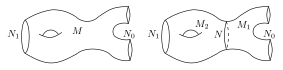
\includegraphics{figures/c1-fig01.svg}

    	\caption{Cutting a manifold $M$ into two manifolds $M_1$ and $M_2$ along
      a codimension-one submanifold $N$. The gluing axiom asserts that
      $Z_M=Z_{M_2} \circ Z_{M_1}$.}
    	\label{f:gluing}
    \end{figure}

    The gluing axiom is a very strong axiom. It allows us to compute the path
    integral of a manifold from smaller pieces. The gluing axiom tells us how
    the (path integrals of) smaller pieces are to be glued along their
    boundaries in order to reconstruct the path integral of the original
    manifold. The underlying assumption that we can compute the path integrals
    of smaller pieces individually makes the locality of the theory manifest.
\end{enumerate}


Note that for the empty space $\varnothing$, the space of fields on
$\varnothing$ is a 1-point set, so $L^2(\calF_\varnothing)=\C$; thus, it is
natural to expect $\calH_\varnothing=\C$. This is also compatible with the
disjoint union axiom, since $\varnothing$ is the unit of the disjoint union
operation: $\calH_{N} \cong \calH_{N \sqcup \varnothing} \cong \calH_{N}\otimes
\calH_{\varnothing}$. Thus, for a closed spacetime (i.e., $\del M=\varnothing$),
we get an operator
\begin{equation}
	Z_M\colon \C\to \C.
\end{equation}
In other words, $Z_M\in \C$ is a number; in physics it is usually called the
\emph{partition function}\index{partition function} and denoted by $Z(M)$.

%%%%%%%%%%%%%%%%%%%%%%%%%%%%%%%%%%%%%%%%
\section{Topological QFT}\label{s:tqft}

So far we have not specified what we mean by ``manifold''. Usually in physics
the spacetime is an oriented pseudo-Riemannian manifold, with a metric of
signature $(1, n-1)$. However, we will be interested in a very special case,
namely when all the structures above do not use the metric on spacetime; thus,
we only require $M$ to be an oriented smooth manifold. Such theories are called
\emph{topological}. The most famous example of such a theory is Chern--Simons
theory\footnote{This is a minor simplification: Chern--Simons theory is not 
  strictly topological -- it has framing anomaly. We will discuss it in 
  more detail in \chref{c:321}} (see \cite{witten-jones}), in which the 
spacetime $M$ must be
3-dimensional, and fields are $\SU(r)$ connections on $M$. After choosing a
trivialization of the bundle, these fields can be described by one-forms,
usually denoted by $A$, with values in the Lie algebra $\su(r)$. The action is
then given by
\begin{equation}
  S[A] = \frac{k}{4 \pi} \int_M \tr(A\wedge dA + \tfrac{2}{3}A\wedge A\wedge A).
\end{equation}

The ``level'' $k$ is a fixed integer parameter of the theory. Although the
numerical value of the Chern--Simons action may change by an integer multiple of
$2\pi k$ under a change of trivialization, the exponentiated action $e^{i S[A]}$
is unchanged. The important thing to note here is that the path integrals
defined using this action do not depend on the choice of the metric. So the
partition functions assigned by this QFT are invariant under
orientation-preserving diffeomorphisms. (It turns out that there are other
observables in this theory besides the partition functions, namely the Wilson
loops, but our preliminary definition of a TQFT does not take these observables
into account.) We can axiomatize the invariance under diffeomorphisms as a
defining property of a topological theory. Together with the axioms of a QFT, we
get the following preliminary definition:

\begin{predefinition}\label{d:ptqft}
  An $n$-dimensional topological quantum field theory (TQFT) is the following
  collection of data:
  \begin{itemize}
    \item For every closed $(n-1)$-dimensional oriented smooth manifold $N$, a
      vector space $Z_N$
    \item For every compact $n$-dimensional oriented manifold $M$ with boundary
      $\del M=\ov{N_0}\sqcup N_1$, a linear operator
      $Z_M\colon Z_{N_0}\to Z_{N_1}$,
  \end{itemize}

  such that

  \begin{itemize}
  	\item Orientation-preserving diffeomorphisms preserve this data
  	\item This data satisfies the disjoint union axiom and the gluing axiom
  	  defined above.
  \end{itemize}

\end{predefinition}

There is a lot more detail to be filled in, but that requires some preparation.
We will provide a more precise definition, due to Atiyah \cite{atiyah}, later
(see \deref{d:tqft}).

Remarkably, topological theories are much easier to define rigorously than
general QFTs. For example, as we show later, in a TQFT all vector spaces
assigned to $(n-1)$-dimensional manifolds are automatically finite-dimensional,
thus avoiding all analytical difficulties with convergence. And instead of
defining a TQFT by a path integral or other global construction (which can be
very hard to do), we can try to construct TQFTs by defining $Z(M)$ for
``elementary blocks'' and gluing every manifold from them. For example, for
$n=2$, any compact oriented surface can be obtained by gluing copies of the
disk, the cylinder, and the pair of pants.
\begin{center}
  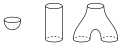
\includegraphics{figures/c1-fig02.svg}
\end{center}

Of course, we need to have some compatibility conditions to ensure that
different ways of gluing the manifold from pieces give the same result;
essentially, we are trying to define manifolds by ``generators and
relations''. For $n=2$ it is not too hard (we will do so in
\chref{c:2d-classification}); for larger $n$, it is harder --- e.g., for
$n=3$ we can consider the so-called Heegaard decompositions (which already
requires infinitely many blocks, namely all handlebodies of arbitrary
genus) or use surgery along (framed) links. The difficulty lies in how fast the data
grows with higher dimensions. Ideally, we would want the number of
generators/relations to be as small as possible in a TQFT, or at least
finite. This leads to the notion of an extended TQFT.

%%%%%%%%%%%%%%%%%%%%%%%%%%%%%%%%%%%%%%%%%%
\section{Toward extended TQFT}\label{s:xtqft}
So far we have talked about cutting a manifold into smaller manifolds with
boundaries. By assigning appropriate data to manifolds with boundaries, we
could glue them back and assign a topological invariant to all possible closed
$n$-manifolds. But why stop at manifolds with boundary? If we allow manifolds
with corners of any codimension, the set of ``elementary blocks'' is greatly
simplified: any manifold can be glued together from just one kind of local
block, namely an $n$-simplex. Such theories are called fully extended (or
sometimes local) TQFTs; see \cite{lurie-cobordism}.

But the price we pay is algebraic complexity. In our discussion so far, a TQFT
assigned a number to a closed $n$-manifold, and a vector space to a
codimension-one manifold. If we also allow cutting along codimension-2
manifolds, what kind of data should be assigned to them? And then what about the
next level?


One possible approach to describing  TQFTs with pieces of any codimensions
is by using the language of higher categories. Very informally, an
$n$-category is an algebraic structure which has objects, 1-morphisms
between them, 2-morphisms between 1-morphisms, and so on, up to
$n$-morphisms. Defining it rigorously quite difficult (we will talk more
about higher categories in \chref{c:higher-cat}). Thus, we could try to
assign to a every zero-dimensional manifold an object of $n$-category, to a
1-dimensional object, a 1-morphism, and so on. This leads to the notion of
\emph{extended TQFT}.


This chapter was roughly centered around the theme that the subject of TQFT
aims to sidestep the analytical difficulties associated with QFTs. One could,
however, also argue for the viewpoint that the mathematical study of TQFTs is
actually a step in dealing with analytical difficulties that the current
formulation of QFT suffers from. In either case, we hope the reader is
convinced that the subject of TQFT lies at a very interesting intersection of
modern physics and mathematics.



\include{c2-categories-src-gerby}
%!TEX root = TQFTnotes.tex
%%%%%%%%%%%%%%%%%%%%%%%%%%%%%%
\chapter{Category of cobordisms and definition of TQFT}\label{c:cobordisms}

In this chapter, we give the key definition of this book, namely the notion of a
TQFT, following work of Atiyah (see \cite{atiyah}). To do that, we first define
the notion of a cobordism.

Unless specified otherwise, ``manifold'' means a compact oriented smooth
manifold, possibly with boundary. For a manifold $M$, we denote by $\del M$ its
boundary, with the orientation determined by the orientation of $M$. If $\del
M=\varnothing$, we say that $M$ is \emph{closed}. Morphisms between manifolds
are smooth maps; unless stated otherwise, ``diffeomorphism'' means an
orientation-preserving invertible smooth map.

We denote by $\ov{M}$ the manifold $M$ considered with the
opposite orientation.

The main references for this chapter are \cite{kock} and
\cite{milnor-h-cobordism}.

%%%%%%%%%%%%%%%%%%%
\section{Category $\nCob$ and definition of TQFT}\label{s:TQFT-def}
\begin{definition}\label{d:cobordism}\index{cobordism}
Let $N_0, N_1$ be closed $(n-1)$-dimensional manifolds. A \emph{cobordism}
from $N_0$ to $N_1$ is an $n$-dimensional manifold $M$ together with
an isomorphism
$$
  \ph\colon \ov{N_0}\sqcup N_1 \isoto \del M.
$$
We will refer to $N_0$ as the incoming boundary (or simply the in-boundary),
and to $N_1$ as the outgoing boundary (out-boundary).

Following \cite{kock}, we will write $N_0\cob{M} N_1$ to indicate that $M$ is a
cobordism from $N_0$ to $N_1$.
\end{definition}

The picture below shows a 2-dimensional cobordism between a circle and a union
of two circles; this cobordism is usually called \emph{pair of pants}\index{pair of pants}.
\begin{center}
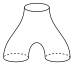
\includegraphics{figures/c3-fig01.svg}
\end{center}

\begin{convention}
In our pictures, cobordisms go ``top to bottom'':
the in-boundary is at the top, and the out-boundary is at the bottom.
\end{convention}

\begin{definition}\label{d:cobordism-isomorphism}\index{cobordism!isomorphism}
  An isomorphism of two cobordisms $M_1, M_2\in \nCob(N_0,N_1)$ is a
  diffeomorphism $f\colon M_1\to M_2$ which makes this diagram commutative:
  \begin{equation}\label{e:cob-iso}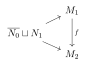
\includegraphics{figures/c3-fig02.svg}\end{equation}
\end{definition}
Given two cobordisms $N_0\cob{M_1}N_1$, $N_1\cob{M_2}N_2$, it is natural to
ask if they can be glued together in a single cobordism $M=M_2\circ M_1$
$$
  N_0\cob{M_2\circ M_1}N_2.
$$
Clearly, as a manifold, $M$ should be obtained by gluing $M_1$ and $M_2$ along
the common boundary $N_1$: $M= M_1\cup_{N_1} M_2$. However, there is a problem:
it is easy to define $M$ as a topological space, but the smooth structure is not
unique. There are several ways to deal with this problem.
\begin{itemize}
  \item One can switch to the category of PL manifolds and cobordisms,
    where the problem does not arise: the PL structure on $M_1\cup_{N_1} M_2$
    is uniquely determined by the PL structures on $M_1$, $M_2$.
  \item One can consider \emph{collared}\index{collared manifold}
    manifolds: instead of
    isomorphism $\ov{N_0}\sqcup N_1\to \del M$,
    we can require in the definition of cobordism an isomorphism of
    $(\ov{N_0}\sqcup N_1)\times [0, \epsilon)$ with a neighborhood
    of $\del M$ in $M$.
\end{itemize}
However, the simplest way is to note that while the smooth structure is not
unique, different smooth structures give isomorphic cobordisms.

\begin{theorem}\label{t:gluing-unique}
  The smooth structure on $M=M_1\cup_{N_1} M_2$ which agrees with
  the given smooth structures on $M_1$, $M_2$, is unique up to isomorphism:
  if $\al, \al'$ are two different smooth structures on $M$, then $(M,\al)$,
  $(M,\al')$ are isomorphic as cobordisms.
\end{theorem}
You can find a proof of this in \cite[Theorem 1.3.12]{kock}.

\begin{definition}\label{d:ncob}\index{cobordism category}
  The cobordism category $\nCob$ is the category whose objects are closed
  $(n-1)$-dimensional manifolds, and $\Hom(N_0, N_1)$ is the set of
  isomorphism classes of cobordisms $N_0\cob{M}N_1$. The composition of
  cobordisms $N_0\cob{M_1}N_1$, $N_1\cob{M_2}N_2$
  is given by
  $$
    M_2\circ M_1 = M_1\cup_{N_1} M_2
  $$
  (by the previous theorem it is independent of the choice of smooth structure).
  The identity morphism $\id_N$ is the cylinder $N\times I$.
\end{definition}
Similarly one defines the PL version of cobordism category.

This category has a natural structure of a symmetric monoidal
category with respect to disjoint union.

\begin{definition}\label{d:tqft}\index{TQFT}
  An $n$-dimensional TQFT is a symmetric
  monoidal functor $Z\colon \nCob\to \vect$.
\end{definition}
This definition was first given in \cite{atiyah} in slightly different
language.

One can also generalize this definition, allowing the TQFT to take values in
other categories.

\begin{definition}\label{d:tqft-c}
  Let $\calC$ be a symmetric monoidal category. Then an
  $n$-dimensional TQFT with values in $\calC$ is a symmetric
    monoidal functor $Z\colon \nCob\to \calC$.
\end{definition}
%%%%%%%%%%%%%%%%%%%%%%%%%%%%
\section{1D TQFT}\label{s:1d-tqft}

Now that we have a definition of a TQFT, let us try to construct examples. We
begin with the simplest possible case, that of a 1-dimensional TQFT.

\begin{theorem}\label{t:1d-TQFT}
  A 1-dimensional TQFT is the following collection of data:
  \begin{itemize}
    \item A vector space $V_+=Z(\bullet^+)$
    \item A vector space $V_-=Z(\bullet^-)$
    \item A linear map $\ev= Z(\cup)\colon V_+\otimes V_-\to \kk$
    \item A linear map $\coev = Z(\cap)\colon \kk \to V_-\otimes V_+$
  \end{itemize}
  satisfying relations below.
  \begin{equation}\label{e:1d-tqft-rigidity}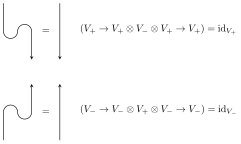
\includegraphics{figures/c3-eqfig01.svg}\end{equation}
\end{theorem}
\begin{proof}
  Since $Z$ is symmetric monoidal, $Z(N_1\sqcup N_2)\simeq Z(N_1)\otimes Z(N_2)$,
  so $Z$ on objects is determined by its values on connected 0-manifolds. The
  only connected 0-manifolds are the positively and negatively oriented points
  $\bullet^+, \bullet^-$, hence $Z$ on objects is determined by
  $V_\pm := Z(\bullet^\pm)$.

  Similarly, $Z$ on morphisms is determined by its values on connected
  cobordisms. Up to isomorphism, every connected oriented $1$-cobordism with
  non-empty boundary is one of the following:
  \begin{itemize}
    \item the intervals $\bullet^+\to\bullet^+$ and $\bullet^-\to\bullet^-$,
      on which $Z$ is the identity of $V_+$ resp.\ $V_-$;
    \item the \emph{cup}
      $\bullet^+\sqcup\bullet^-\to\varnothing$, on which $Z$ is a linear
      map $\ev\colon V_+\otimes V_-\to\kk$;
    \item the \emph{cap}
      $\varnothing\to\bullet^-\sqcup\bullet^+$, on which $Z$ is a linear
      map $\coev\colon \kk\to V_-\otimes V_+$.
  \end{itemize}
  The only connected closed $1$-cobordism is the circle $S^1$; its value
  $Z(S^1)\in\kk$ will turn out to be determined by the data above.

  It remains to identify the relations these data must satisfy. The snake
  cobordism on the left-hand side of the first equation of
  \eqref{e:1d-tqft-rigidity} is diffeomorphic (rel boundary) to the straight
  interval on the right-hand side; applying $Z$ to this diffeomorphism gives
  the first snake identity. The second is obtained analogously by reversing
  orientations.

  Conversely, given data $(V_+, V_-, \ev, \coev)$ satisfying
  \eqref{e:1d-tqft-rigidity}, one defines $Z$ on objects and connected
  cobordisms by the formulas above and extends to general objects and
  morphisms by tensor product and composition. The relations
  \eqref{e:1d-tqft-rigidity} ensure that the result is independent of the
  decomposition; with this, $Z$ is well-defined as a symmetric monoidal
  functor $\oneCob\to\vect$.
\end{proof}

\begin{lemma}\label{l:rigidity_vect}
  Let $V_+, V_-$, $\ev, \coev$ be as in \thref{t:1d-TQFT}.
  Then $V_+, V_-$ are finite-dimensional, and
  one can identify $V_-=V_+^*$ so that $\ev, \coev$ become the usual
  evaluation and coevaluation maps $V\otimes V^*\to \kk$,
  $\kk\to V\otimes V^*\colon 1\mapsto \sum e_i\otimes e^i$.
\end{lemma}
\begin{proof}
  Consider the map $V_-\to (V_+)^*$, given by $y\mapsto \ev(-,y)$; and a map
  $V_+^*\to V_-$ given by
  $f\mapsto \id \otimes f (\coev(1))$ (thus, if $\coev(1)=\sum y_i \otimes x_i$,
  then $f\mapsto \sum f(x_i) y_i$). Then the rigidity conditions say that these
  two maps are inverse to each other; thus, we have $V_-\simeq V_+^*$.
  Finite-dimensionality follows from the fact that the elements $y_i$ generate
  $V_-$.
\end{proof}
Thus, a one-dimensional TQFT is completely determined by a
\emph{finite-dimensional} vector space $V=Z(\bullet^+)$; in such a
TQFT, $Z(S^1)=\dim V$.


%%%%%%%%%%%%%%%%%%%%%%%%%
\section{Rigid monoidal categories}\label{s:1d-tqft-rigid}
In the previous section, we had shown that a 1d TQFT with values in the category
of vector spaces is uniquely determined by the vector space $V=Z(\bullet^+)$,
which must be finite-dimensional. What happens if we now consider TQFTs with
values in an arbitrary monoidal category $\calC$?

It turns out that there is a very similar answer, but with finite-dimensionality
replaced by the following condition.

\begin{definition}\label{d:dual-object}
  Let $\calC$ be a monoidal category.
  A \emph{dual pair}\index{dual pair} is a pair of objects $A,B\in \calC$
  together with morphisms
  \begin{align*}
    \ev&\colon A\otimes B\to \one \qquad \text{(evaluation morphism),}\\
    \coev&\colon \one \to B\otimes A \qquad \text{(coevaluation morphism)},
  \end{align*}
  satisfying the \emph{rigidity}\index{rigidity} condition below.
  \begin{equation}\label{e:rigidity}
    \begin{aligned}
      &\Bigl(B\to \one\otimes B \xto{\coev\otimes 1_B}
                       (B\otimes A)\otimes B \xto{\al_{B,A,B}}
                       B\otimes (A\otimes B) \xto{1_B\otimes \ev}
                       B\otimes \one \to
                       B\Bigr) = 1_B\\
      &\Bigl(A\to  A\otimes \one  \xto{1_A\otimes \coev}
                       A\otimes (B\otimes A) \xto{\al^{-1}_{A,B,A}}
                       (A\otimes B)\otimes A \xto{\ev\otimes 1_A}
                       \one\otimes A \to
                       A\Bigr) = 1_A
    \end{aligned}
  \end{equation}
  In this situation we say that $A$ is a
  \emph{left dual}\index{dual object!left} of $B$, and
  $B$ is a \emph{right dual}\index{dual object!right} of $A$.
\end{definition}

It is common to represent the evaluation and coevaluation graphically:
\begin{equation}\label{e:ev-coev-graphical}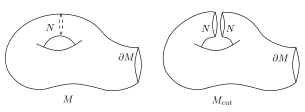
\includegraphics{figures/c3-fig03.svg}\end{equation}

Then the rigidity equations \eqref{e:rigidity} are illustrated by
\begin{equation}\label{e:rigidity2}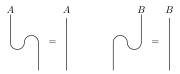
\includegraphics{figures/c3-eqfig02.svg}\end{equation}



It turns out that right dual, if exists, is unique up to unique isomorphism.
\begin{theorem}\label{t:dual_unique1}
  Let $(A, B, \ev, \coev)$ and $(A,B', \ev', \coev')$ be two dual pairs with
  the same $A$.
  Then there exists a unique morphism $\ph\colon B\to B'$ such that
  $\ev = \ev' \circ (1_A\otimes \ph)$,
  $\coev' =(\ph\otimes 1_A) \coev$.
\end{theorem}
The proof is a standard snake-diagram argument: the required $\ph$ is given by
the composition
$$
  B \xto{1_B\otimes \coev'} B\otimes A\otimes B'
    \xto{\ev\otimes 1_{B'}} B',
$$
and uniqueness follows by chasing the rigidity equations.
A similar statement holds for left dual.

This allows us to talk about the right dual of $A$ as a well-defined object in
$\calC$. We will denote the right dual of $A$ by ${}^*A$; similarly we will use
notation $B^*$ for left dual of $B$. In this notation, evaluation and
coevaluation morphisms become
\begin{equation}
  \begin{aligned}
    \ev&\colon X^*\otimes X\to\one\\
    \coev&\colon \one \to X\otimes X^*.
  \end{aligned}
\end{equation}

Clearly, in a symmetric monoidal
category, the left dual is also a right dual.

\begin{definition}\label{d:rigid}
  An object $A$ in a monoidal category $\calC$ is
  \emph{rigid}\index{rigid object} if
  it has both left and right duals.

  A monoidal category is \emph{rigid}\index{monoidal category!rigid}
  if every object is rigid.
\end{definition}

\begin{example}\label{x:vector-rigid}
  A vector space $V$ is rigid as an object of $\vect$ if and only if it is
  finite-dimensional.
\end{example}


\begin{exercise}\label{ec:coev-unique}
  Show that in a dual pair, the coevaluation is uniquely determined by
  the remaining data: if $(A, B, \ev, \coev)$ and $(A,B, \ev, \coev')$
  are dual pairs, then $\coev = \coev'$.

  Similarly, $\ev$ is uniquely determined by $(A,B, \coev)$.
\end{exercise}

\begin{exercise}\label{ec:dual-of-tensor}
  Let $X^*$, $Y^*$ be right duals of objects $X, Y$. Show that then $X\otimes Y$
  also has a right dual, and there is a canonical isomorphism $(X\otimes
  Y)^*\simeq Y^* \otimes X^*$.
\end{exercise}

\begin{exercise}\label{ec:dual-morphism}
  Let $\calC$ be a rigid monoidal category. For a morphism $f\colon X\to Y$,
  define a morphism $f^*\colon Y^*\to X^*$ by the picture below.

  \begin{equation}\label{e:dual-morphism}
\includegraphics{figures/c3-fig04.svg}\end{equation}


  Prove that then
  $(fg)^*=g^* f^*$; thus, $*$ is a contravariant functor $\calC\to \calC$.
\end{exercise}

After these preliminaries, we can now easily classify 1-dimensional TQFTs with
values in any symmetric monoidal category.

\begin{theorem}\label{t:1d-tqft}
  If $Z\colon \oneCob\to \calC$ is a $1$-dimensional TQFT with values in a
  symmetric monoidal category $\calC$, then $A=Z(\bullet^+)$ is a rigid object;
  its dual is $Z(\bullet^-)$. Conversely, any rigid object $A\in \calC$ defines
  a one-dimensional TQFT such that $Z(\bullet^+)=A$.
\end{theorem}

%\begin{tikzpicture}
%  \begin{scope}[tikzdefault]
%  \draw[->] (-0.5,0) arc (-180:0:0.5);
%  \draw[-] (0.5,0) arc (0:180:0.5);
%  \end{scope}
%\end{tikzpicture}


%%%%%%%%%%%%%%%%%%%%%
\section{First properties of TQFTs}\label{s:first-properties}



Let us now try to establish some properties of general $n$-dimensional TQFTs.

\begin{theorem}\label{t:tqft-rigidity}
  Let $Z\colon \nCob\to \calC$ be an $n$-dimensional TQFT with values in a
  symmetric monoidal category $\calC$. Then for any closed $(n-1)$-dimensional
  manifold $N$, $Z(N)\in \calC$ is rigid, and $Z(\ov{N})$ is a dual of $Z(N)$.
\end{theorem}
The proof is the same as in the one-dimensional case.

In particular, for TQFTs with values in $\vect$, for any closed
$(n-1)$-dimensional manifold $N$, the vector space $Z(N)$ is finite-dimensional.

\begin{exercise}\label{ec:tqft-duality}
  Let $Z$ be an $n$-dimensional TQFT with values in $\vect$. Prove that then
  $Z(N\times S^1)=\dim Z(N)$ for any closed $(n-1)$-dimensional manifold $N$.
\end{exercise}

Note that unlike the one-dimensional case, in general we cannot claim that any
rigid object of $\calC$ defines a TQFT. The proper generalization of that
statement is the cobordism hypothesis, which we will discuss later.



Another property of TQFTs is functoriality. As mentioned before, it is
natural to expect that a diffeomorphism $\ph \colon N_0\to N_1$ between two
$(n-1)$-dimensional closed manifolds gives rise to an isomorphism
$Z(\ph)\colon Z(N_0)\to Z(N_1)$; however, we didn't include that as part of
the definition. It turns out it is not necessary.

Let $\ph \colon N_0\to N_1$ be a diffeomorphism. Define the cobordism
\begin{equation}\label{e:Cph}
  N_0\cob{C_\ph} N_1
\end{equation}
to be the cylinder $N_1\times I$, with the identification $\ov{N_0}\sqcup N_1
\to \del C_\ph$ given by $\ph\sqcup \id$.

\begin{lemma}\label{l:tqft-isotopy}
  Let $C_\ph$ be defined above. Then:
  \begin{enumerate}
    \item The isomorphism class of $C_\ph$ \textup{(}as a cobordism\textup{)} only depends on the
    isotopy class of $\ph$: if $\ph, \ph'$ are isotopic to each other, then
      $C_\ph\simeq C_{\ph'}$.
    \item Given diffeomorphisms $\ph_1\colon N_0\to N_1$, $\ph_2\colon N_1\to
      N_2$, we have an isomorphism of cobordisms
      $$
        C_{\ph_2}\circ C_{\ph_1}\simeq C_{\ph_2 \ph_1}.
      $$
  \end{enumerate}
\end{lemma}
Recall that $\ph, \ph'$ are called isotopic if there exists a one-parameter
family $\ph_t$ of smooth maps $N_0\to N_1$ such that $\ph_t$ is a diffeomorphism
for all $t$, and $\ph_0=\ph$, $\ph_1=\ph'$.

We leave the proof of this lemma as an easy exercise to the reader.

\begin{remark}
  In fact, there is a stronger statement: $C_\ph\simeq C_{\ph'}$ if and only if
  $\ph, \ph'$ are \emph{pseudo-isotopic}\index{pseudo-isotopic}, see
  \cite[Theorem 1.9]{milnor-h-cobordism}.
\end{remark}




As an immediate corollary, we get the following theorem.
\begin{theorem}\label{t:tqft-functoriality}
  Let $Z\colon \nCob\to \calC$ be an $n$-dimensional TQFT.
  \begin{enumerate}
    \item For any diffeomorphism $\ph\colon N_0\to N_1$, define
      $Z(\ph)\colon Z(N_0)\to Z(N_1)$ by $Z(\ph)=Z(C_\ph)$. Then
      $Z(\ph_2\ph_1)= Z(\ph_2)\circ Z(\ph_1)$.
    \item If $\ph_0,\ph_1$ are isotopic, then $Z(\ph_0)=Z(\ph_1)$.
  \end{enumerate}
\end{theorem}
\clearpage


\part{TQFTs in 2 dimensions}\label{p:2d}
%!TEX root = TQFTbook.tex
%%%%%%%%%%%%%%%%%%%%%%%%%%%%%%
In this part, we start building the theory of extended TQFTs, i.e., theories
where we consider not just cobordisms but manifolds with corners. In this part
we are mostly working with 2-dimensional extended TQFTs, leaving higher
dimensional case for the following part.

To give an accurate definition of such an extended TQFT in dimension 2, one
needs to introduce the language of (weak) 2-categories, which we do in
\chref{c:2categories}. We also introduce the notion of a symmetric monoidal
2-category. Our key examples of 2-categories are the 2-category of small
categories (or a variation of it, the 2-category of all locally finite
$\kk$-linear abelian categories) and the category $\Alg$, whose objects are
algebras over $\kk$ and 1-morphisms are bimodules. Both 2-categories play an
important role in future constructions.

Next, in \chref{c:duality-2cat} we discuss dualities in 2-categories, discussing
both the notion of a dual object (which only makes sense in a monoidal
2-category) and of a dual 1-morphism; in particular, we show that for the
2-category of small categories, where 1-morphisms are functors between
categories, so defined duality coincides with the classical notion of
adjointness for functors.
In \chref{c:separable-frobenius}, we study the duality in the 2-category $\Alg$
and show that fully dualizable objects in $\Alg$ are the separable algebras;
moreover, fixing a duality between $\ev$ and $\coev$ 1-morphisms is equivalent
to choosing a structure of a Frobenius algebra, which provides the link to the
construction of (non-extended) TQFTs done earlier.


After completing all these preliminaries, we finally define the notion of an
extended 2d TQFT in \chref{c:2d-extended}. Following work of Schommer--Pries, we
construct the set of generators and relations for the 2-category $\Bord_2$ of
2-dimensional bordisms and use it to show that extended 2d TQFTs are classified
by separable symmetric Frobenius algebras.

Finally, in \chref{c:PL}--\chref{c:2d-lattice} we present an alternative
approach to construction of extended 2d TQFTs. Instead of using Morse functions
to create a presentation of a cobordism as a composition of elementary
cobordisms, we use triangulations (or more generally, PL cell decompositions);
instead of Cerf moves, we use Pachner moves. We show how in dimension 2, it
gives a very explicit construction of an extended 2d TQFT from a separable
symmetric Frobenius algebra $A$, providing a different way of proving the same
classification result.
%!TEX root = TQFTnotes.tex
%%%%%%%%%%%%%%%%%%%%%%%%%%%%%%
\chapter{Classification of 2d TQFT}\label{c:2d-classification}
In this chapter, we present a full classification of 2-dimensional TQFTs; the
final answer, given in \thref{t:2d-classification2}, states that such theories
are classified by commutative Frobenius algebras. This is a relatively simple
result; it goes back to at least 1989, see Dijkgraaf's thesis
\cite{dijkgraaf-thesis}, but was probably known to experts much earlier. For
us, it will serve as a model example for all future constructions.

For a two-dimensional TQFT, there is only one $1$-dimensional oriented closed
manifold: the circle $S^1$, and any orientation-preserving diffeomorphism
$S^1\to S^1$ is isotopic to the identity. It also seems obvious (and in fact
can be justified using Morse theory, as we discuss below)  that any
cobordism can be obtained by gluing pieces diffeomorphic to one of the
cobordisms below together with the cylinder $S^1\times I$:
\begin{center}
  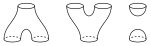
\includegraphics{figures/c4-fig01.svg}
\end{center}

It is also not hard to write some relations, such as the
associativity relation

\begin{equation}\label{e:2d-assoc-prelim}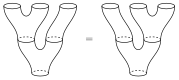
\includegraphics{figures/c4-fig02.svg}\end{equation}


However, how can one show that this is the full list of relations?

There are two approaches. One, used in \cite{kock}, uses the classification of
surfaces; using that, we show that the relations we have are enough to bring any
composition of generators to some canonical form. This approach does not require
much beyond the classification of surfaces, but it does not generalize to
higher dimensions.

There is, however, an alternative approach, based on Morse and Cerf theory.
This goes back at least to \cite{abrams}, who used a handle-decomposition
viewpoint to give a classification of 2d TQFTs; the Cerf-theoretic version
is presented in \cite{moore-segal} and \cite[Lecture~23]{freed-bordism},
the latter of which our exposition follows. One can also find more details
in the unpublished paper \cite{gay-wehrheim-woodward}.

%%%%%%%%%%%%%%%%%%%%%%%%%%%%%%
\section{Morse theory basics}\label{s:morse}

We start with an overview of Morse theory; details can be found, e.g., in
\cite{matsumoto}.

Recall that given a smooth real-valued function $f$ on an $n$-dimensional
manifold $M$, a point $p\in M$ is a \emph{non-degenerate critical point}
\index{critical point!non-degenerate} if
$\del_i f (p)=0$ and the Hessian matrix
$a_{ij}=\frac{\del^2 f}{\del  x^i \del x^j}(p)$ is non-degenerate. It is easy to
see that this is independent of the choice of coordinate system. It is also
known that in such a case, one can choose local coordinates in a neighborhood
of $p$ so that
\begin{equation}\label{e:crit-point}
  f(x^1, \dots, x^n)=c-(x^1)^2 -\dots -(x^r)^2
  + (x^{r+1})^2+ \dots + (x^n)^2
\end{equation}
(this statement is usually called the \emph{Morse lemma}\index{Morse lemma}).
The number $r$ of minuses in \eqref{e:crit-point} is called the \emph{index}
of the critical point.

It is immediate from the definition that a non-degenerate critical point
is isolated; thus, if $M$ is compact, there can be only finitely many
non-degenerate critical points.

\begin{definition}\label{d:morse_function}\index{Morse function}
  Let $M$ be a closed $n$-manifold. A Morse function is a
  smooth function $f\colon M\to \R$ such that all critical points
  of $f$ are non-degenerate.
\end{definition}

It will be more useful to impose a stronger condition.

\begin{definition}\label{d:morse_function2}
  Let $M$ be a closed $n$-manifold. A Morse function  $f\colon M\to \R$
  is called \emph{excellent}\index{Morse function!excellent} if all critical
  values $c_i=f(p_i)$ are distinct.
\end{definition}

It was proved by Morse that such functions exist; moreover, the set $\calF^0$
of excellent functions is an open and dense subset in $C^\infty(M)$
(in an appropriate topology).

We can generalize the notion of excellent functions to manifolds with boundary,
or to cobordisms $N_0\cob{M} N_1$.

\begin{definition}\label{d:morse-function3}
  Let $N_0\cob{M} N_1$ be an $n$-dimensional cobordism. A Morse function on $M$
  is a smooth function $f\colon M\to \R$ such that
  \begin{itemize}
    \item $f$ is constant on both in-boundary and out-boundary:
      $f|_{N_0}=a_0=\min_M f$, $f|_{N_1}=a_1=\max_M f$
    \item All critical points of $f$ are in the interior
      $M\setminus (N_0\cup N_1)$, and all critical points are non-degnerate.
  \end{itemize}
  If, in addition, all critical values of $f$ are distinct, then $f$ is called
  \emph{excellent}.
\end{definition}
 Again, one can prove
that such functions exist and form an open dense subset of all functions
satisfying $f|_{N_0}=a_0$, $f|_{N_1}=a_1$.

The main result of Morse theory is that given an excellent function $f$, the
topology of the manifold $M_t=f^{-1}((-\infty, t])$ does not change between
critical values: if $c_i<c_{i+1}$ are critical values, with no other critical
values between them, then for all $t\in I=[c_i+\eps, c_{i+1}-\eps]$, the
manifolds $M_t$ are diffeomorphic, and $M_I=f^{-1}(I)\isoto N_{t_0} \times I$,
where $N_{t_0}=f^{-1}(t_0)$ is a slice for any $t_0\in I$. Moreover, one can
give an explicit description of how topology of $M_t$ changes when one  goes
through a critical point (this is usually referred to as ``attaching a
handle''). In particular, this implies that if $f$ has no critical points, then
$M$ is a cylinder: $M\isoto N\times I$.

Therefore, one can use Morse functions to decompose a cobordism as a
composition of ``elementary'' cobordisms.
\begin{definition}\label{d:elem-cobordism}\index{elementary cobordism}
  An elementary cobordism is a cobordism that admits a Morse  function
  with a single  critical point.
\end{definition}

Thus, given an excellent function with critical values $c_1<\dots<c_k$,
and values on the boundary $f|_{N_0}=a_0<c_1$, $f|_{N_1}=a_k>c_k$, we
can choose intermediate values $a_i\in (c_i, c_{i+1})$; then we have
\begin{equation}\label{e:morse-decomposition}
  M=M_k\circ \dots \circ M_1,
\end{equation}
where $M_i=f^{-1}([a_{i-1}, a_i])$ is the elementary cobordism containing
critical point $p_i$. It follows from the result above that up to
isomorphism, $M_i$ does not depend on the choice of $a_i$. We will refer to
\eqref{e:morse-decomposition} as a
\emph{Morse decomposition}\index{Morse decomposition} of a cobordism.

In particular, for $n=2$, each connected elementary cobordism is isomorphic to
one of the four cobordisms shown in Table~\ref{tab:elementary-2cob}. Note that
here we follow our convention that cobordisms go ``top to bottom''; thus, the
$y$-axis is directed downward, so that the minimal value of $f$ is at the top,
and the maximal, at the bottom.
\begin{table}[ht]
  \centering
  \setlength{\extrarowheight}{8pt}%
  \begin{tabular}{|l|l|}
    \hline
    Index  & Elementary cobordism \\
    \hline
    0 &
    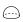
\includegraphics{figures/c4-fig03.svg} \\[8pt]
    \hline
    1 &
    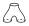
\includegraphics{figures/c4-fig04.svg} \qquad
    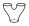
\includegraphics{figures/c4-fig05.svg} \\[12pt]
    \hline
    2 &
    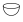
\includegraphics{figures/c4-fig06.svg} \\[8pt]
    \hline
  \end{tabular}
  \medskip
  \caption{Connected elementary $2$-cobordisms}
  \label{tab:elementary-2cob}
\end{table}
A (not necessarily connected) elementary cobordism is obtained as a disjoint
union of one of the connected elementary cobordisms and  several copies of the
identity cobordism, i.e., $S^1\times I$.

Thus, we see that a choice of an excellent function gives a presentation of a
2-cobordism as a composition of the generators shown in
Table~\ref{tab:elementary-2cob} (and identity cobordisms).

%%%%%%%%%%%%%%%%%%%%%%%%%%%%%%%%%%%%
\section{Cerf theory}\label{s:cerf}

We have seen that excellent Morse functions allow one to present a cobordism as
a composition of elementary cobordisms; for $n=2$, this gives us a set of
generators for the category of cobordisms.



To describe relations between generators, we need to see how one can go from
one such presentation to another, or equivalently, how the presentation changes
if we replace one excellent Morse function by another.

It is easy to see that the space of excellent functions is not connected; thus,
if $f_0$, $f_1$ are two excellent functions, and we want to connect them by a
path $f_s$, $s\in [0,1]$ in the space of functions, in general this path must go
through some points which are not excellent. This was studied by Cerf in
\cite{cerf} and is usually referred to as \emph{Cerf theory}\index{Cerf
theory}.

\begin{example}\label{x:morse-x3}
  Consider the one-parameter family of functions $f_s= x^3+sx$ on a neighborhood
  of the origin in $\R$, with local coordinate $x$, shown in \firef{fig:x3}.

  Then for $s<0$, the function is Morse with two critical points of indices
  $0$ and $1$ respectively; for $s>0$, it is also Morse, with no critical
  points; and for $s=0$, $f_0(x)=x^3$ is not a Morse function: zero is a
  degenerate critical point. Thus, in this case, $f_s$, considered as a path in
  the function space, connects two Morse functions but goes through a non-Morse
  function $f_0=x^3$. This path describes annihilation of a pair of critical
  points (or, going in the opposite direction, birth of a pair of critical
  points).

  \begin{figure}[ht]
    \centering
    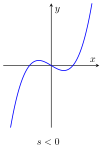
\includegraphics{figures/c4-fig07.svg}
    \qquad
    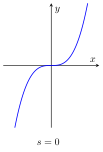
\includegraphics{figures/c4-fig08.svg}
    \qquad
    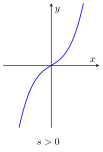
\includegraphics{figures/c4-fig09.svg}
    \caption{Birth-death of critical points in family  $f_s=x^3+sx$}
    \label{fig:x3}
  \end{figure}


\end{example}

\begin{example}\label{x:morse-crossing}
  Consider the family of  functions $f_s(x)=x^2-x^4+sx$. Then for values of $s$
  close to 0, it has three  critical points, all of them non-degenerate: local
  minimum at $p_0$ close to 0, and local maxima at points $p_1<0$, $p_2>0$.

  For $s<0$, we have $c_1>c_2$; for $s>0$, $c_1<c_2$, and for $s=0$, $c_1 = c_2$
  as shown below, so for $s=0$ this function is Morse but not excellent. Thus,
  we again get a path connecting two excellent functions going through a
  non-excellent function with $c_1=c_2$.

  \begin{figure}[ht]
    \centering
    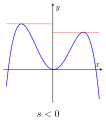
\includegraphics{figures/c4-fig10.svg}
    \qquad
    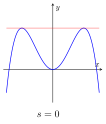
\includegraphics{figures/c4-fig11.svg}
    \qquad
    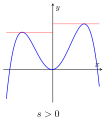
\includegraphics{figures/c4-fig12.svg}

    \caption{Crossing of critical values in family $f_s=x^2-x^4+sx$}
    \label{fig:x4-x2}
  \end{figure}

\end{example}

It turns out that these two model examples are enough: any two excellent
functions can be connected by a one-parameter family where all non-excellent
functions are at worst as in these examples. More precisely, we have the
following.

\begin{definition}\label{d:morse-good}
  A \emph{good}  function on an $n$-dimensional closed manifold $M$ is a
  smooth function of one of the following types:
  \begin{itemize}
    \item {\bf Type $\alpha$}: all critical values are distinct, and all
      critical points are non-degenerate, except for one. Near this point,
      there is a local coordinate system where $f$ is given by
      $$
      f(x^1, \dots, x^n)=c+(x^1)^3 -(x^2)^2-\dots -(x^r)^2+(x^{r+1})^2 +
                        \dots +(x^n)^2.
      $$
    \item {\bf Type $\beta$}: all critical points are non-degenerate, and
      all critical values are distinct except for one pair: $c_i = c_j$
      for some $i\ne j$.
  \end{itemize}
  In a similar way one defines good function on a cobordism $M$.
\end{definition}

(The name ``good'' is not standard.)

It was shown by Cerf that this is the beginning of a stratification of the
space $\calF=C^\infty(M)$: we can write
$\calF = \calF^0\sqcup \calF^1\sqcup\dots$,
where $\calF^0$ is the set of excellent functions, which is open and dense in
$\calF$; the set $\calF^1$ consists of good functions and is a codimension 1
subset of $\calF$, and so on. (One can also define higher codimension strata,
but we will not need them.) A review of this theory can be found, e.g., in
\cite[Section I.2]{hatcher-wagoner}.

\begin{theorem}\label{t:cerf1}
  Let $f_0, f_1$ be two excellent functions on a cobordism $M$. Then one can
  find a one-parameter family $f_s$ of smooth functions on $M$ such that:
  \begin{enumerate}
    \item $f_s$ is excellent for all $s$ except for finitely
      many values $s_1, \dots, s_p$
    \item At each of these special values, $f_s$ is good.
  \end{enumerate}
\end{theorem}
In other words, any two points in $\calF^0$ can be connected by a path
contained in $\calF^0\cup \calF^1$.

Moreover, this path can be chosen so that it is transversal to $\calF^1$ (we
skip the precise definition, referring the reader to \cite{hatcher-wagoner}).
This allows one to describe how the Morse decomposition changes when we cross
one of the components of $\calF^1$ (``walls''). Crossing a component
corresponding to a type-$\alpha$ function produces a \emph{birth-death move}:
two adjacent critical points (of indices $r-1, r$) appear or disappear.
Crossing a component corresponding to a type-$\beta$ function produces a
\emph{crossing move}: two critical values $c_i, c_{i+1}$ exchange their order.

\begin{theorem}\label{t:cerf}
  Let $M$ be a cobordism, and let $f_0, f_1$ be two excellent functions on
  $M$, with corresponding Morse decompositions $\calD_0$, $\calD_1$ as in
  \eqref{e:morse-decomposition}. Then $\calD_0$ and $\calD_1$ can be obtained
  from each other by a finite sequence of birth-death moves and crossing
  moves and their inverses.
\end{theorem}


%%%%%%%%%%%%%%%%%%%%%%%%%%%%%%%%%%%%%%%%
\section{Generators and relations of $\twoCob$}\label{s:2cob-relations}

Now let us apply the general theory above to the question of classification
of 2d TQFTs.

First, choosing an excellent Morse function on a 2d cobordism $M$, we get a
decomposition of $M$ into a composition of elementary cobordisms. Each elementary
cobordism is a disjoint union of copies of the connected elementary cobordisms;
and each connected elementary cobordism is isomorphic to one of the standard
cobordisms shown in Table~\ref{tab:elementary-2cob}: pair of pants, copants,
cap, and cup.

Let us denote by $A=Z(S^1)$ the vector space associated to the circle, and by
$m, i, \Delta, \eps$ the linear operators corresponding to the standard
cobordisms as shown below.

\begin{equation}\label{e:frobenius-data}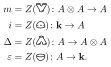
\includegraphics{figures/c4-eqfig01.svg}\end{equation}


Then a choice of an excellent Morse function $f$ on $M$, together with a choice
of isomorphism $\ph_i$ of each of the connected elementary cobordisms defined by
$f$ with one of the ``standard'' ones, gives us a presentation of $Z(M)$ as a
composition of tensor products of operators $m, i, \Delta, \eps$
(and the identity operator $\id_A$).
Therefore, the structure of TQFT is completely determined by these 4 operators.
Note also that $m$ and $\Delta$ are symmetric: $m\circ P= m$, where
$P\colon A\otimes A\to A\otimes A$ is the permutation
$P(a\otimes b)= b\otimes a$. Indeed, this follows from the isomorphism of
cobordisms shown below: the standard copants surface admits a self-diffeomorphism
(a $180^\circ$ rotation about its central vertical axis) that swaps the two
input boundary circles and fixes the output boundary circle.
\begin{equation}\label{e:m-symmetric}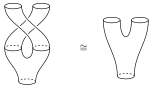
\includegraphics{figures/c4-fig13.svg}\end{equation}
The analogous argument applied to the pants surface (turn the picture upside
down) gives $P\circ\Delta = \Delta$.

Next, observe that the choice of isomorphisms $\ph_i$ is in fact irrelevant.
Indeed, since any orientation-preserving diffeomorphism $\ph$ of $S^1$ is
isotopic to the identity, by \leref{l:tqft-isotopy} its action on $A$ is trivial:
$\ph_*=\id_A$. From this it immediately follows that if $M$ is topologically a
disk, considered as a cobordism $\varnothing \cob{} S^1$ (i.e., a cap), then the
operator $Z(M)\colon \kk \to A$ does not depend on the choice of the isomorphism
of $M$ with the standard cap; a similar result holds for the cup.

If $M$ is a cobordism $S^1\sqcup S^1\to S^1$ which is isomorphic to the
standard pair of pants, there are just two isomorphisms up to isotopy; one is
obtained from the other by composing with the diffeomorphism that interchanges
the two circles that form the in-boundary. But since $m$ is symmetric as
discussed above, both choices of isomorphism give us the same operator
$Z(M)=m\colon A\otimes A\to A$. A similar statement holds for the cobordism
$S^1\cob{} S^1\sqcup S^1$.

Summarizing, we see that for any cobordism $M$, the presentation of $Z(M)$ as a
composition of tensor products of $m, i, \Delta, \eps$ only depends on the
choice of an excellent Morse function and does not depend on any additional
data.

Thus, to check that $Z(M)$ does not depend on any choices, we need to check
that $Z(M)$ is invariant under the Cerf moves described in \thref{t:cerf}. Let
us analyze what these moves look like for $n=2$.

The birth-death moves (type $\alpha$) are easily seen to be of one of the
following two types:
\begin{center}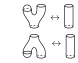
\includegraphics{figures/c4-eqfig02.svg}\end{center}

Now let us consider the crossing move. Assume that we have a family of Morse
functions $f_s$ and two critical points $p_1, p_2$ such that for $s<0$,
$c_1<c_2$, for $s>0$, $c_1>c_2$, and for $s=0$, $c_1=c_2=c$. Choose some
$a_0<c$, $a_1>c$ and consider the (non-elementary) cobordism
$M=f_{0}^{-1}[a_0, a_1]$.

Since operators of the form $X\otimes 1$ and $1\otimes Y$ commute anyway, if
the points $p_1, p_2$ are in different connected components of the cobordism
$M$, then the crossing move does not give any new conditions on
$m, i, \Delta, \eps$.
Therefore, we only need to consider the case when the two critical points $p_1,
p_2$ are in the same connected component of the critical level set
$S=f_0^{-1}(c)$. This immediately implies that each of the critical points is of
index 1.

The set $S$ is a smooth curve except at critical points, where $S$ looks like a
coordinate cross; thus, $S$ is a graph with two 4-valent vertices $p_1$, $p_2$.
Moreover, since $M$ is oriented, we can define an orientation on $S$ (for
example, defining the tangent vector $v$ to $S$ by the condition that $(v, \grad
f)$ is a positively oriented frame). Orientation also gives a cyclic order of
edges at each vertex $p_i$. Using Morse lemma, it is easy to see that
near each critical points $S$ looks as shown below:
\begin{equation}\label{e:S-local}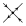
\includegraphics{figures/c4-fig14.svg}\end{equation}

\begin{lemma}\label{l:critical-level}
  Let $S$ be a connected directed graph with two vertices $p_1, p_2$ of degree
  4, together with a cyclic order of edges at each vertex, such that near each
  vertex it is locally isomorphic to the graph shown in \eqref{e:S-local}.

   Then $S$ is isomorphic to one of the four graphs shown in
   \firef{f:critical-level}, and their orientation reversals.
\end{lemma}
The proof of this lemma is an  elementary combinatorics argument; we leave
details  to the reader.


\begin{figure}[ht]
  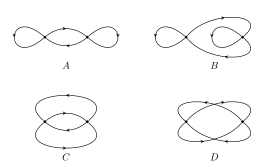
\includegraphics{figures/c4-fig15.svg}
  \caption{Possible shapes of critical level set $S$. Note that for the last
  graph, intersection points are not vertices.}\label{f:critical-level}
\end{figure}


Each of these graphs uniquely determines the corresponding connected component
of the cobordism $M=f_0^{-1}(c-\eps, c+\eps)$; we can recover it by replacing
each arc of the graph by a thin ribbon. For example, for graph A, the
corresponding cobordism is shown below (for reader's convenience, we also show
it in a more familiar form):
\begin{center}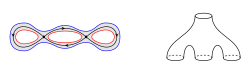
\includegraphics{figures/c4-eqfig03.svg}\end{center}

In this case, one easily sees that the corresponding Cerf move is given by
\begin{center}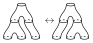
\includegraphics{figures/c4-eqfig04.svg}\end{center}
Reversing the orientation of the graph $A$ is equivalent to flipping the picture
in the vertical direction, which gives the Cerf move below:
\begin{center}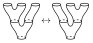
\includegraphics{figures/c4-eqfig05.svg}\end{center}

Similarly, graph $B$ gives the following Cerf move:
\begin{center}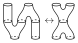
\includegraphics{figures/c4-eqfig06.svg}\end{center}

Graphs $C$ and $D$ are less obvious. For $C$, the cobordism $M$ is of type 2-2:
it is a surface of genus zero, with two circles as in-boundary, and two circles
as out-boundary. However, in this case, the Cerf move looks like:
\begin{center}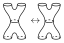
\includegraphics{figures/c4-eqfig07.svg}\end{center}
In other words, both for $s<0$ and for $s>0$ in the family of Morse functions
$f_s$, the corresponding Morse decomposition of the cobordism is a composition
of copants and pants. Thus, it gives no new conditions on $m, \Delta$.

Similarly, graph $D$ gives a cobordism of genus 1 from $S^1$ to $S^1$; again,
in this case both for $s<0$ and for $s>0$ the Morse decomposition looks like

\begin{center}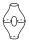
\includegraphics{figures/c4-eqfig08.svg}\end{center}
and thus the corresponding Cerf move gives no new conditions on $m,\Delta$.

Summarising, we see that the non-trivial Cerf moves (both birth-death and
crossings) for $n=2$ are shown in \firef{f:cerf-dim2}. In this table, we also
include the algebraic identities on the operators $m, i, \Delta, \eps$ (defined
by \eqref{e:frobenius-data}) corresponding to each of the moves.

\begin{figure}[ht]
\centering
\renewcommand{\arraystretch}{1.4}
\begin{tabular}{lcl}
  \hline
  \textbf{Name} & \textbf{Cerf move} & \textbf{Algebraic identity}\\
  \hline
  %%%%%%%%%%%%%%%%%%%%%
  Unit &
    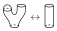
\includegraphics{figures/c4-fig16.svg}
    & $m\circ (i\otimes \id_A) = \id_A$\\[10pt]
  %%%%%%%%%%%%%%%%%%%%%
  Counit &
    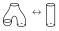
\includegraphics{figures/c4-fig17.svg}
    & $(\eps\otimes \id_A)\circ \Delta = \id_A$\\[10pt]
  %%%%%%%%%%%%%%%%%%%%%
  Associativity &
    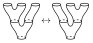
\includegraphics{figures/c4-fig18.svg}
    & $m\circ (m\otimes \id_A) = m\circ (\id_A\otimes m)$\\[20pt]
  %%%%%%%%%%%%%%%%%%%%%
  Coassociativity &
    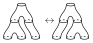
\includegraphics{figures/c4-fig19.svg}
    & $(\Delta\otimes \id_A)\circ \Delta = (\id_A\otimes \Delta)\circ
    \Delta$\\[20pt]
  %%%%%%%%%%%%%%%%%%%%%
  Frobenius &
    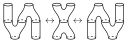
\includegraphics{figures/c4-fig20.svg}
    & $\begin{aligned}
        \Delta\circ m
          &= (m\otimes \id_A)\circ (\id_A\otimes \Delta)\\
          &= (\id_A\otimes m)\circ (\Delta\otimes \id_A)
      \end{aligned}$\\[20pt]
  \hline
\end{tabular}
\caption{Cerf moves in dimension 2 and
         the corresponding algebraic identities}\label{f:cerf-dim2}
\end{figure}

It is easy to see that the identities given by the  unit and associativity moves
are equivalent to the statement that $m, i$ define on $A=Z(S^1)$ a structure of
an associative algebra. Similarly, coassociativity and counit say that $\Delta,
\eps$ define on $A$ a structure of coassocaitive coalgebra.

Combining these identities with the symmetry relations $m\circ P = m$,
$P\circ \Delta = \Delta$ established in \eqref{e:m-symmetric}, we obtain the
following theorem.


\begin{theorem}\label{t:2d-classification}
  A 2d TQFT is equivalent to the following collection of data.
  \begin{itemize}
    \item A vector space $A=Z(S^1)$.
    \item Linear maps $m\colon A\otimes A\to A$, $i\colon \kk\to A$.
    \item Linear maps $\De\colon A\to A\otimes A$, $\eps\colon A\to \kk$.
  \end{itemize}
  This data has to satisfy the following conditions:
  \begin{itemize}
    \item $(A,m, i)$ is a commutative algebra with unit; as usual, we will use
      the notation $ab$ as a shorthand for $m(a\otimes b)$.
    \item $(A,\De, \eps)$ is a cocommutative coalgebra with counit.
    \item The Frobenius condition
      \begin{equation}\label{e:frobenius}
        \De(a_1 a_2) = (a_1\otimes 1) \De(a_2)= \De(a_1)(1\otimes a_2).
      \end{equation}
  \end{itemize}
\end{theorem}

\begin{remark}\label{r:frobenius-two}
  Since $\Delta, m$ are symmetric, any one of the two Frobenius relations
  implies the other; we include both for use in the more general case.
\end{remark}


\begin{remark}\label{r:2d-commutative}
  Note that commutativity of $m$ and cocommutativity of $\Delta$ do not come
  from any of the Cerf moves in \firef{f:cerf-dim2}; they follow from the
  symmetric-pants argument \eqref{e:m-symmetric} (and its mirror image), which
  in turn reflects the symmetric monoidal structure of $\twoCob$.
\end{remark}


A standard way to restate the above theorem is using the notion of Frobenius
algebra.
\begin{definition}\label{d:frobenius}\index{Frobenius algebra}
  A Frobenius algebra is a vector space over a field $\kk$ with two structures:
  \begin{itemize}
    \item A structure of an associative algebra, with multiplication $m$ and
      unit $i\colon \kk \to A$.
    \item A structure of a coassociative coalgebra, with comultiplication $\De$
      and counit $\eps\colon A\to \kk$.
  \end{itemize}
  These two structures must satisfy the Frobenius condition \eqref{e:frobenius}.
\end{definition}
Note that in this definition, we do not assume that $A$ is commutative or
cocommutative.

Then \thref{t:2d-classification} can be rewritten as follows.
\begin{theorem}\label{t:2d-classification2}
  A 2d TQFT is equivalent to a commutative, cocommutative Frobenius algebra.
\end{theorem}
In the next section we will show that cocommutativity follows from
commutativity, so it is enough to require $A$ to be commutative; see
\coref{c:frobenius-commutative}.


\clearpage

%!TEX root = TQFTnotes.tex
%%%%%%%%%%%%%%%%%%%%%%%%%%%%%%
\chapter{Frobenius algebras}\label{c:frobenius}


In the previous chapter, we have shown that 2-dimensional TQFTs are classified
by commutative, cocommutative Frobenius algebras. In this chapter, we will study
Frobenius algebras in detail.


Recall that a Frobenius
algebra is a vector space over a field $\kk$ with two structures (see
\deref{d:frobenius}):
\begin{itemize}
  \item A structure of an associative algebra, with multiplication $m$ and
    unit $i\colon \kk \to A$.
  \item A structure of a coassociative coalgebra, with comultiplication $\De$
    and counit $\eps\colon A\to \kk$.
\end{itemize}
These two structures must satisfy the Frobenius condition
\eqref{e:frobenius}.

Note that the Frobenius condition can be restated as follows. Define on
$A\otimes A$ an  $A$-bimodule structure by $x (a_1\otimes a_2) = (xa_1)\otimes
a_2$, $(a_1\otimes a_2) x = a_1\otimes (a_2 x)$. Then the Frobenius condition
is equivalent to the following:
\begin{equation}\label{e:frobenius2}
  \De\colon A\to A\otimes A \text{ is a morphism of $A$-bimodules.}
\end{equation}
Note that in this definition, we do not assume that $A$ is commutative or
cocommutative.

\begin{remark}
  Given a vector space with structures of an associative algebra and
  coassociative coalgebra, there are several natural choices for
  compatibility between these two structures. By far the most commonly used
  ones are
  \begin{itemize}
    \item \emph{Bialgebra condition}:
      the comultiplication is a morphism of algebras.
      (Frequently one also requires existence of a certain involution, called
      the \emph{antipode}\index{antipode}; this gives the definition of a Hopf
      algebra\index{Hopf algebra}.)
      Examples of bialgebras include group algebras, universal
      enveloping algebras of  Lie algebras, and more.
    \item \emph{Frobenius condition}: the comultiplication is a morphism
      of $A$-bimodules.
  \end{itemize}
  These are different choices: a Frobenius algebra is not the same as a
  Hopf algebra. They both have their uses; for 2d TQFT, we need the
  structure of a Frobenius algebra.
\end{remark}


%Let us spend some time studying Frobenius algebras. We will use the
%following graphical presentation of operations in a Frobenius algebra.
%
%\begin{equation}
%  \begin{tikzpicture}
%    \pic{mult};
%    \pic at (1.5,0) {comult};
%  \end{tikzpicture}
%\end{equation}


We will use a graphical presentation of various algebraic
operations, representing linear operators $A^{\otimes k}\to A^{\otimes m}$
by graphs with $k$ legs at the top and $m$ legs at the bottom (thus, our
operators act ``from top to bottom'').

\firef{f:graphical1} shows
graphs used to represent  the  common algebraic operations.
\begin{figure}[ht]
  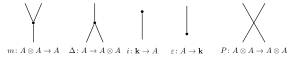
\includegraphics{figures/c5-fig01.svg}
%  \begin{tikzpicture}
%    % bilinear form
%    \node (E1) at (-0.5, 0.5) {};
%    \draw (E1) -- +(0,-0.5)  arc (180:360:0.5cm) --+(0,0.5);
%    \node at (1,0) {$=$};
%    \node[dotnode] (E2) at (1.5,0){};
%    \draw (E2)--+(-0.3,0.7);
%    \draw (E2)--+(0.3,0.7);
%    \draw (E2)--+(0,-0.5) node[dotnode]{};
%    \node[scale=0.8] at (0.5,-1) {$(\, , \,)\colon A\otimes A\to \kk$};
%    % e
%    \node (F1) at (3,-0.5) {};
%    \draw (F1) -- +(0,0.5)  arc (180:0:0.5cm) --+(0,-0.5);
%    \node at (4.5,0) {$=$};
%    \node[dotnode] (F2) at (5,0){};
%    \draw (F2)--+(0,0.5) node[dotnode]{};
%    \draw (F2)--+(-0.3,-0.7);
%    \draw (F2)--+(0.3,-0.7);
%    \node[scale=0.8] at (4, -1) {$e=\De(1)\in A\otimes A$};
%    % casimir
%    \node[dotnode] (om) at (7,0) {};
%    \draw (om) arc(-90:270:0.4cm);
%    \draw (om)--+(0,-0.7);
%    \node[scale=0.8] at (7, -1) {$E=m(e)\in A$};
%  \end{tikzpicture}

  \caption{Graphical presentation of operations in a Frobenius algebra. $P$
  stands for permutation: $P(a\otimes b)=b\otimes a$.}\label{f:graphical1}
\end{figure}


Thus, the Frobenius relation \eqref{e:frobenius} is graphically represented by
\begin{equation}\label{e:frobenius-graphical}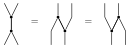
\includegraphics{figures/c5-eqfig01.svg}\end{equation}


\section{Frobenius pairing}\label{s:frobenius-pairing}
It turns out that there is an alternative definition of Frobenius algebras.


\begin{theorem}\label{t:frobenius1}
  Let $A$ be a Frobenius algebra. Then $A$ is finite-dimensional
  and the bilinear pairing
  \begin{equation}\label{e:frob-pairing-thm}
    (a,b) = \eps(ab)
  \end{equation}
  is non-degenerate; the corresponding coevaluation map
  $\kk \to A\otimes A$ is given by $\De \circ i$.
\end{theorem}

We will use ``cup'' and ``cap'' graphics to denote the pairing $\eps(ab)$
and the coevaluation $\De \circ i$:
\begin{equation}\label{e:fr-cap-cup}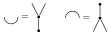
\includegraphics{figures/c5-eqfig02.svg}\end{equation}
\begin{proof}
  Define maps $\ev\colon A\otimes A \to \kk$ and $\coev\colon \kk\to A\otimes A$
  by \eqref{e:fr-cap-cup}. Then it immediately follows from the Frobenius
  relation that these maps satisfy the rigidity condition:
  \begin{equation}\label{e:frob-rigidity}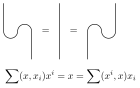
\includegraphics{figures/c5-eqfig03.svg}\end{equation}
  where $x_i, x^i$ are defined by $\De(1)=\sum x_i \otimes x^i$.
  Thus, by  \leref{l:rigidity_vect}, $A$ is finite-dimensional, and $\eps(ab)$
  is a non-degenerate pairing.

\end{proof}






As an immediate corollary, we see that the comultiplication is uniquely
determined by the unit, the multiplication, and the counit. Indeed, by
\thref{t:frobenius1},
$e= \De(1)$ is given by
\begin{equation}\label{e:e1}
  e= \De(1) = \sum x_i \otimes x^i
\end{equation}
where $x_i, x^i$ are dual bases in $A$ with respect to the Frobenius pairing:
$(x^i,x_j)=\de_{ij}$. On the other hand, it follows from the Frobenius
relation that
\begin{equation}\label{e:Delta}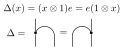
\includegraphics{figures/c5-eqfig04.svg}\end{equation}

\begin{exercise}\label{ec:frobenius-dual-basis}
  Let $A$ be a Frobenius algebra, and let $x_i, x^i$ be as in \eqref{e:e1}.
  \begin{enumerate}
    \item Define the map $\la\colon A\otimes A \otimes A \to \kk$ by
      $\la(a_1\otimes a_2\otimes a_3)= \eps(a_1a_2a_3)$:
      \begin{equation}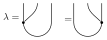
\includegraphics{figures/c5-eqfig05.svg}\end{equation}
      Let $c_{ijk}=\la(x_i, x_j, x_k)=\eps(x_i x_j x_k)$.

      Prove that then the structure constants of the multiplication and the
      comultiplication are obtained by ``raising indices'' of $c_{ijk}$:
      \begin{align*}
        x_i x_j &= \sum c_{ijk}g^{kl}x_l =\sum g^{lk}c_{kij}x_l,\\
        \De(x_i)&= \sum c_{ijk}g^{jj'}g^{kk'}x_{k'}\otimes x_{j'}
                = \sum c_{jki}g^{j'j}g^{k'k}x_{k'}\otimes x_{j'}
      \end{align*}
      where $g^{ji}$ is the inverse matrix of $g_{ij}=(x_i, x_j)$ (thus, $x^i =
      \sum g^{ij}x_j$). Note that we do not assume that $g_{ij}$ is symmetric.
    \item
      Prove that the comultiplication is also given by the picture below:
      \begin{equation}\label{e:fr-comultiplication}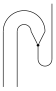
\includegraphics{figures/c5-fig02.svg}\end{equation}
  \end{enumerate}
\end{exercise}

\begin{corollary}\label{c:frobenius-commutative}
  If a Frobenius algebra  $A$ is commutative, it is also cocommutative.
\end{corollary}

Conversely, one can recover the structure of a Frobenius lagebra from the
pairing $(, \, \,)$.

\begin{theorem}\label{t:frobenius2}
  Let $A$ be a finite-dimensional associative algebra and let $\eps\colon A\to
  \kk$ be a linear map such that the bilinear pairing $(a,b) = \eps(ab)$ is
  non-degenerate. Let $e= \sum x_i \otimes x^i\in A\otimes A$, where $x_i, x^i$
  are dual bases with respect to $(\, , \,)$: $(x^i, x_j)= \de_{ij}$. Then $e$
  is central: $(a\otimes 1)e = e (1\otimes a)$, and  $A$ has a canonical
  Frobenius algebra structure with the comultiplication given by
  \eqref{e:Delta}.
\end{theorem}
\begin{proof}
The sequence of pictures below gives a graphical proof that $e$ is central; we
leave it to the reader to rewrite it algebraically:
\begin{equation}\label{e:e-central-graphical}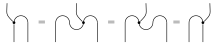
\includegraphics{figures/c5-fig03.svg}\end{equation}
  Coassociativity, the counit axiom, and the Frobenius property are proved by
  very similar computations, which we leave to the reader.
\end{proof}
Thus, we could give an alternative definition of a Frobenius algebra.
\begin{definition}\label{d:frobenius2}\index{Frobenius algebra}
  A Frobenius algebra is a finite-dimensional associative algebra
  $A$ together with a map $\eps \colon A\to \kk$ such that the
  bilinear pairing
  \begin{equation}\label{e:frob-pairing}
    (a,b) = \eps(ab)
  \end{equation}
  is non-degenerate.
\end{definition}
By Theorems \ref{t:frobenius1} and \ref{t:frobenius2}, this is equivalent to the
previously given definition (\deref{d:frobenius}).

There are also many other equivalent definitions of Frobenius
algebras; see, e.g., \cite[Section 2.2]{kock}.

Note that while in general, the pairing $(a,b) = \eps(ab)$ need not
be symmetric, in most examples of interest to us it is.
\begin{definition}\label{d:frobenius_symmetric}
  A Frobenius algebra $A$ is \emph{symmetric}\index{Frobenius
  algebra!symmetric} if $\eps$ is trace-like, i.e.,
  $$
    \eps(ab)=\eps(ba).
  $$
\end{definition}
Of course, every commutative Frobenius algebra is symmetric;
however, the examples below show that an algebra can be
symmetric without being commutative.

\begin{example}\label{x:frobenius1}
  Let $A=\C[x]/(x^{n+1})$, with $\eps(x^k)=1$ if $k=n$ and
  $\eps(x^k)=0$ otherwise. This is a commutative Frobenius algebra which
  has a natural topological interpretation: it is the cohomology of
  $\C P^n$. In particular, for $n=1$, this Frobenius algebra and the
  corresponding TQFT play an important role in the theory of Khovanov
  homology.
\end{example}
\begin{example} \label{x:frobenius2}
  Let $A$ be the algebra of $n\times n$ matrices over $\kk$,
  with $\eps(a)=\la\cdot\tr(a)$, for some $\la\ne 0$. Then $A$
  is a symmetric Frobenius algebra.
\end{example}

The following lemma is immediate from the definition.
\begin{lemma}\label{l:bicentral}
  Let $A$ be  a symmetric Frobenius algebra, and let
  $e=\sum x_i\otimes x^i\in A\otimes A$ be as in \thref{t:frobenius2}. Then
  \begin{enumerate}
    \item $e$ is symmetric: $P(e)=e$, where $P\colon A\otimes A\colon a\otimes
    b\mapsto b\otimes a$.
    \item $e$ is \emph{bicentral}\index{bicentral}:
    \begin{align*}
      \sum ax_i\otimes x^i&=\sum x_i\otimes x^i a,\\
      \sum x_ia\otimes x^i&=\sum x_i\otimes ax^i.
      \end{align*}
    \end{enumerate}
\end{lemma}
%%%%%%%%%%%%%%%%%%%%%%%%%%%%%%%%%%%%%%%%%
\section{Semisimple Frobenius algebras}\label{s:frobenius-ss}

Recall that an associative algebra is semisimple if it is a direct sum of simple
algebras.  As we will see later, semisimple algebras play a special role in the
construction of TQFTs, so in this section, we study \textbf{semisimple}
Frobenius algebras. We have already seen one example: the Frobenius algebra
$A=\Mat_n(\kk)$ given in \exref{x:frobenius2}. In fact, over an algebraically
closed field, it is the most general example of a semisimple symmetric Frobenius
algebra. Namely, we have the following lemma.

\begin{lemma}\label{l:frobenius-ss}\index{Frobenius algebra!semisimple}
  Let $\kk$ be an algebraically closed field.
  Then any semisimple symmetric Frobenius algebra $A$ has the form
  $$
    A=\bigoplus_i \Mat_{n_i}(\kk)
  $$
  where $\Mat_n(\kk)$ is the algebra of $n\times n$ matrices, and
  $$
  \eps(a)=\sum_i \la_i \tr(a_i)
  $$
  for some constants $\la_i\ne 0$, where $a_i\in\Mat_{n_i}(\kk)$ is the
  $i$-th component of $a$.
\end{lemma}
Indeed, by the Wedderburn theorem (see e.g., \cite[Section 3.5]{pierce}), any
finite-dimensional semisimple algebra over $\kk$ is a direct sum of matrix
algebras, and it is well known that for a matrix algebra, $A/[A,A]$ is
one-dimensional, which easily implies the statement of the lemma.

In particular, this gives us the following classification
of semisimple commutative Frobenius algebras.

\begin{theorem}\label{t:frobenius_commutative}
  Let $\kk$ be an algebraically closed field. Then
  any semisimple commutative Frobenius algebra over $\kk$ has the following
  form
  $$
  A=\bigoplus_{i=1}^n \kk e_i, \quad e_ie_j=\de_{ij}e_i
  $$
  with unit $1=\sum_i e_i$ and counit
  $$
  \eps(e_i)=\la_i, \quad \la_i\ne 0.
  $$
\end{theorem}

It is an easy exercise to show that for an algebra described in
\thref{t:frobenius_commutative}, the canonical element $e=\De(1)$ is given by
$$
e= \sum_i \la_i^{-1}e_i\otimes e_i
$$
and the comultiplication is given by
$$
\De(e_i)=\la_i^{-1}e_i\otimes e_i.
$$
In particular, it implies that for the corresponding TQFT, we have
\begin{align*}
  Z(S^2)&=\eps(1)=\sum \la_i\\
  Z(T)&=\dim A
\end{align*}
where $T=\Si_1$ is the two-dimensional torus.

\begin{lemma}\label{l:semisimple_theory}
  Let $A$ be as in \thref{t:frobenius_commutative}, and let $Z_A$ be
  the corresponding 2d TQFT. Then for a closed surface $\Si_g$ of genus $g$,
  we have
  $$
  Z_A(\Si_g) = \sum_i \la_i^{1-g}.
  $$
\end{lemma}
\begin{proof}
  The cases $g=0, 1$ have already been discussed. For general $g\ge 1$, it is
  easy to see that $Z_A(\Si_g)=\tr(W^{g-1})$, where $W\colon A\to A$ is given by
  $W = Z_A(\Si_{1,2})$, with $\Si_{1,2}$ a torus with one in-boundary circle and
  one out-boundary circle:
  \begin{center}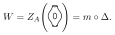
\includegraphics{figures/c5-eqfig06.svg}\end{center}
  Using the formula for comultiplication, we see that $W(e_i)=\la_i^{-1}e_i$,
  which immediately gives the statement of the lemma.
\end{proof}
\begin{remark}
  It is easy to see that the operator $W$ defined above
  coincides with the operator of multiplication
  by the element $w=m\circ \Delta (1)$. Explicitly,
  this element can be described by
  \begin{equation}\label{e:euler}
    w=\sum x_ix^i \in A,
  \end{equation}
  where $x_i$, $x^i$ are dual bases in $A$ with respect to the pairing. This
  element is sometimes called the \emph{Euler element}\index{Euler element}
  and will play an important role later, see \thref{t:separable-frobenius}.
  (In \cite{lauda-pfeiffer}, $w$ is called the ``window element''.)
\end{remark}

\begin{exercise}\label{ec:dual-module-frob}
  Recall that for an $A$-$B$-bimodule $M$, the dual vector space $M^*$
  is naturally a $B$-$A$-bimodule, with action given by
  \begin{align*}
    (b\la) (m) & = \la (mb),\\
    (\la a) (m) &= \la (am).
  \end{align*}
  In particular, the dual of an $A$-bimodule is again an $A$-bimodule.

  Let $A$ be a symmetric Frobenius algebra.
  \begin{enumerate}
    \item
      Show that the map $A\to A^*\colon a\mapsto (a, -)$ is a morphism of
      $A$-bimodules.
    \item
      More generally, let $M$ be a finite-dimensional left $A$-module. Let
      $M^\vee =\Hom_A(M, A)$; it has a natural structure of a right
      $A$-module. Show that then the map below is an isomorphism of right
      $A$-modules: %FIXME
      \begin{align*}
        M^\vee &\to M^*\\
        f&\mapsto \eps(f(-)).
      \end{align*}
      and the inverse is given by
      \begin{align*}
        M^* &\to M^\vee\\
        \la&\mapsto \sum \la(x_im)x^i,
      \end{align*}
      where $x_i, x^i$ are as in \eqref{e:e1}.
  \end{enumerate}
\end{exercise}
\clearpage

\include{c6-DW-src-gerby}
%!TEX root = TQFTnotes.tex
%%%%%%%%%%%%%%%%%%%%%%%%%%%%%%
\chapter{2-categories}\label{c:2categories}

In the previous chapters, we classified all 2d TQFTs; the key step of this
classification was the fact that any cobordism can be obtained by composing a
small set of generating cobordisms (cup, cap, pants, copants). However, for
higher dimensions, this approach becomes hard; even for $n=3$, it is impossible
to produce a finite set of generating cobordisms.

A possible way out is rethinking the very idea of a cobordism. After all, the
initial physical motivation for TQFT was coming from path integral formulation,
which shows that the invariant of a closed $n$-manifold can be computed by
cutting the manifold into small local pieces, computing the path integral over
each of them (with appropriate boundary conditions) and summing up. Thus, we
just need to  formalize the idea of ``gluing the manifold from local pieces''.
For this, the notion of a cobordism is not enough.

One possible way of defining ``local pieces'' is using the notion of a manifold
with corners. For $n=2$, such a manifold could look like the one shown below:

%% definition of 2-category of bordisms
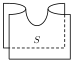
\includegraphics{figures/c7-fig01.svg}

This is a manifold with corners; you can think of it as a cobordism from the
union of two arcs at the top to the union of two intervals at the bottom. Each
of them is not a closed manifold but a 1d cobordism. Thus, for 2-dimensional
TQFT,  we have a structure where we have
\begin{itemize}
  \item 0-dimensional manifolds (corners)
  \item 1-dimensional cobordisms between them
  \item 2-dimensional cobordisms between 1d cobordisms
\end{itemize}

The appropriate language for describing this kind of structures is the
language of 2-categories. In this chapter, we give an overview of the theory
of 2-categories; we refer the reader to \cite{leinster} for details.

%%%%%%%%%%%%%%%%%%%%%%%%%%%%%%%%
\section{Strict 2-categories}\label{s:2cat-strict}
\begin{predefinition}\label{d:2-cat-prelim}
  A 2-category is the following collection of data:
  \begin{enumerate}
    \item A class $\calC_0$, called objects of $\calC$.
    \item For any $X,Y\in \calC_0$, a set $\Hom_{\calC}(X,Y)$,
    called 1-morphisms of $\calC$.
    \item For any pair of 1-morphisms $f,g\in \Hom_\calC(X,Y)$, a set
      $\Hom^2_{\calC}(f,g)$; elements of this set are called
      2-morphisms of $\calC$.
    \item Appropriate composition laws and identity morphisms for 1-
      and 2-morphisms.
  \end{enumerate}
\end{predefinition}
Before giving the full definition, here are the motivating examples ---
whatever definition we give, it must cover these examples (possibly with minor
technical modifications).

\begin{example}\label{x:cat}
  The 2-category $\cat$ of all (small) categories. Objects of this category are
  categories, 1-morphisms are functors, and 2-morphisms are functorial
  morphisms.
\end{example}
\begin{example} \label{x:alg}
  The 2-category $\Alg$ of algebras and bimodules. Objects of this category are
  unital associative algebras (not necessarily finite-dimensional) over a fixed
  ground field $\kk$, 1-morphisms $M\colon A\to B$ are $B$-$A$-bimodules,
  and 2-morphisms are morphisms of bimodules. Composition of 1-morphisms
  is given by tensor product over the algebra:
  $$
  ({}_CM_B, {}_BN_A)\mapsto {}_C M\otimes_B N_A
  $$
  (we use subscripts such as ${}_BN_A$ to indicate that $N$ is a left module
  over $B$ and a right module over $A$.)

  The identity 1-morphism from $A$ to $A$ is $A$ itself considered as an
  $A$-bimodule.
\end{example}
\begin{example} \label{x:2groupoid}
  Let $X$ be a topological space. Define its \emph{fundamental
  2-groupoid}\index{fundamental 2-groupoid} $\Pi_{\leq 2}(X)$ to be the
  following 2-category:
  \begin{itemize}
    \item Objects: points $x\in X$
    \item 1-morphisms: paths $\ga\colon I \to X$ between points
    \item 2-morphisms: equivalence classes of homotopies between paths
          (two homotopies are equivalent if there is a ``homotopy between
          homotopies'' between them)
  \end{itemize}
\end{example}

Morphisms and 2-morphisms in a 2-category are frequently presented graphically.
There are two approaches to it:
\begin{enumerate}
  \item Objects are represented by points, 1-morphisms by arrows,
    and 2-morphisms by 2-cells. This is the more common way.

  \item Objects are represented by regions in the plane, 1-morphisms by lines
    separating these regions (``domain walls''),
    and 2-morphisms by points where these lines meet (or by boxes).
    This approach is very familiar to physicists.
\end{enumerate}

Following \cite[Appendix A.4]{schommer-pries}, we will call diagrams of the
first kind \emph{pasting diagrams} and diagrams of the second kind \emph{string
diagrams}. In both cases, we will accept the convention that 1-morphisms go
``from left to right'', and 2-morphisms go ``from top to bottom''. The figure
below (borrowed with modifications from \cite{schommer-pries}) shows a
comparison of these two types of graphical presentation.

\begin{figure}[ht]
  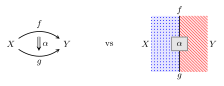
\includegraphics{figures/c7-fig02.svg}
  \caption{Pasting Diagrams vs String Diagrams}
\end{figure}

To turn \deref{d:2-cat-prelim} into a rigorous definition, we need to
define compositions for 1-morphisms and 2-morphisms and state appropriate
associativity and unit laws. There are a couple of subtle points; for
example, for 2-morphisms we need not only composition of 2-morphisms
shown below (vertical composition)
\begin{figure}[h]
  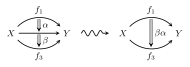
\includegraphics{figures/c7-fig03.svg}
\end{figure}

\noindent
but also ``horizontal composition'', which we denote by $\be\ccirc \al$
to distinguish it from the vertical composition:
\begin{figure}[h]
  
\includegraphics{figures/c7-fig04.svg}
\end{figure}

We can save some effort if we start by saying that for given objects
$X,Y$, all 1-morphisms between them, together with 2-morphisms between those,
form a category. That takes care of (vertical) composition of 2-morphisms,
identity 2-morphism, etc.

\begin{definition}\label{d:2-cat-strict}\index{2-category!strict}
  A strict 2-category $\calC$ is the following collection of data:
  \begin{itemize}
    \item A class of objects $\calC_0$
    \item For any $X, Y\in \calC_0$, a category $\Hom_{\calC}(X,Y)$. Objects of
      this category are called $1$-morphisms from $X$ to $Y$; morphisms
      of $\Hom_{\calC}(X,Y)$ are called $2$-morphisms of $\calC$
    \item A (horizontal) composition functor
      $$
        H\colon \Hom(X,Y)\times \Hom(Y,Z)\to \Hom(X,Z)
      $$
    \item For every $X\in \calC$, an identity 1-morphism $1_X\in \Hom(X,X)$
  \end{itemize}
  such that the horizontal composition is associative and $1_X$ is a unit
  for this composition.
\end{definition}
Instead of providing a $1$-morphism $1_X\in \Hom(X,X)$, we can say
``we have a functor $\one\to\Hom(X,X)$'', where $\one$ is the category
with a single object and a unique morphism (namely, the identity morphism).

Note that since composition is a functor, it also gives a horizontal
composition of 2-morphisms; thus, this is automatically taken care of --- no
need to add horizontal composition of 2-morphisms by hand.

The exact meaning of ``horizontal composition is associative'' is as follows.
For any $X,Y,Z,W\in \calC$, one can construct two functors
$$
\Hom(X,Y)\times \Hom(Y,Z)\times\Hom(Z,W)\to \Hom(X,W)
$$
namely, $H\circ (H\times \id)$ and $H\circ (\id \times H)$. Associativity
means that these two functors are equal. Similarly one can write down the exact
meaning of ``$1_X$ is a unit for horizontal composition''.

\begin{exercise}\label{ec:exchange_condition}
  Consider the pasting diagram below. Then there are two obvious ways to
  compose the four 2-morphisms in this diagram into a single 2-morphism from
  $f_2f_1$ to $g_2g_1$: either using horizontal composition first or using
  vertical composition first. Prove that the resulting 2-morphisms are equal.

  \begin{figure}[h]
    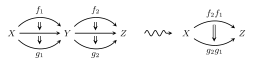
\includegraphics{figures/c7-fig05.svg}
  \end{figure}
  This is known as the ``exchange condition''; it is a special case of the
  so-called \emph{pasting theorem}; broadly speaking, this theorem claims that given a
  composable pasting diagram, the result of composition does not depend on the order
  in which we are doing the compositions. Formulating it precisely is somewhat
  technical; see \cite{power-pasting}.
\end{exercise}
\begin{lemma}\label{l:eckmann-hilton}
  Let $X$ be an object in a strict 2-category $\calC$. Consider the monoid of
  2-morphisms $\Hom(1_X, 1_X)$. Then horizontal and vertical compositions
  coincide, and the resulting composition is commutative.
\end{lemma}
This is known as the \emph{Eckmann--Hilton argument}\index{Eckmann--Hilton argument}; see
\cite[Lemma 1.2.4]{leinster}. It can be viewed as a categorical analog of
the well-known topological fact: for $k>1$, homotopy groups $\pi_k(X)$
are commutative.

\begin{exercise}\label{ec:algebra-in-2cat}
  Let $A$ be an associative algebra, considered as an object in the 2-category
  $\Alg$. Prove that then $\Hom_{\Alg}(1_A, 1_A)=z(A)$ is the center of $A$.
\end{exercise}
%%%%%%%%%%%%%%%%%%%%%%%%%%%%%
\section{Weak 2-categories}\label{s:weak-2cat}
There is one problem with the notion of strict 2-category: this definition is
too strict. For example, in the proposed 2-category of algebras and bimodules,
the identity 1-morphism $1_A\in \Hom(A,A)$ is $A$ considered as an $A$-bimodule.
But if $M$ is an $A$-$B$-bimodule, $A\otimes_A M$ is not equal to $M$: it is only
isomorphic. Thus, we need to relax the associativity condition for composition
of 1-morphisms, similarly to what we did with the associativity condition for
monoidal categories.

\begin{definition}\label{d:2-cat-weak}
  A \emph{weak 2-category}\index{weak 2-category} (also called a bicategory) $\calC$ is the following
  collection of data:
  \begin{itemize}
    \item A class of objects $\calC_0$
    \item For any $X, Y\in \calC_0$, a category $\Hom_\calC(X,Y)$. Objects of
      this category are called $1$-morphisms from $X$ to $Y$; morphisms of
      $\Hom_\calC(X,Y)$ are called $2$-morphisms of $\calC$
    \item A (horizontal) composition functor
      $$
        H\colon \Hom(X,Y)\times \Hom(Y,Z)\to \Hom(X,Z)
      $$
    \item For every $X\in \calC_0$, an identity 1-morphism $1_X\in \Hom(X,X)$
    \item For any quadruple of objects $X,Y,Z,W\in \calC$, an isomorphism
      $\al$ of functors $H\circ (H\times \id)$ and $H\circ (\id \times H)$,
      both considered as functors
      $$
        \Hom(X,Y)\times \Hom(Y,Z)\times\Hom(Z,W)\to \Hom(X,W).
      $$
    \item Left and right unit isomorphisms
  \end{itemize}
  which satisfy the pentagon and triangle axioms.
\end{definition}
The pentagon and triangle axioms are similar to those for a monoidal category;
details can be found, e.g., in \cite[Section 1.5]{leinster}.

\begin{example}\label{x:weak-2cat-examples}\par\noindent
  \begin{enumerate}
    \item The 2-category $\Alg$ of algebras and bimodules,
      introduced in \exref{x:alg}, is
      indeed a weak 2-category.
    \item The 2-category $\cat$ of (small) categories,
      introduced in \exref{x:cat}, is indeed a weak 2-category.
    \item As a variation of the above, we can define a weak 2-category $\ab_\kk$
      of $\kk$-linear abelian categories, together with $\kk$-linear functors
      between them. We can also impose some additional restrictions, such as
      local finiteness (all $\Hom$ spaces are finite-dimensional, and every
      object has finite length) or semisimplicity.
  \end{enumerate}
\end{example}
\begin{example}\label{x:BC}
  Let $\calC$ be a monoidal category. Define the 2-category $\calB\calC$ as the
  2-category with one object $*$ and morphisms given by $\Hom_{\calB\calC}(*,*)
  =\calC$, with horizontal composition given by tensor product.
  It is easy to see that this is indeed a 2-category;
  conversely, every 2-category with only one object is obtained in this
  way. This is sometimes called \emph{delooping}\index{delooping} of $\calC$.
\end{example}

\begin{remark}\label{r:BG}
    The notation $\calB\calC$ is motivated by the following. Let $M$ be a
    monoid (for example, a group). Define the category $\calB M$ as the
    category with a single object $*$ and $\Hom(*,*)=M$. Then it is immediate
    from the definition that for a group $G$, the so-defined category is
    equivalent to the fundamental groupoid of the classifying space $BG$:
    $\calB G\simeq \Pi_1(BG)$; therefore, $\calB$ is the categorical analog of
    the classifying space construction.

  The word ``delooping'' is justified by the following observation: for a
  path-connected topological space $X$, let $\Omega X$ be the space of based
  loops in $X$. Then we have a homotopy equivalence $\Omega BG \simeq G$; thus,
  in some sense $B$ is the inverse operation to $\Omega$, hence the name
  ``delooping''.
\end{remark}

One can also define the notion of functor between (weak) 2-categories,
which we skip, referring the reader to \cite[Definition 1.5.8]{leinster}.
(Note: what we will be using is called ``weak lax functors'' in
\cite{leinster}.) This allows one to define the notion of equivalence of weak
2-categories.

\begin{theorem}\label{t:strictify-bicategories}
  Any weak 2-category is equivalent to a strict 2-category.
\end{theorem}
This theorem is similar to the coherence theorem \thref{t:strictify}; we refer
the reader to \cite[Theorem 1.5.15]{leinster} for the proof.

\begin{remark}\label{r:stictify-3-cat}
  Do not let this theorem give you the wrong idea. For $n=3$, the notion of a
  weak $3$-category (which is quite hard to define, see
  \cite{gordon-power-street}) is not equivalent to that of a strict 3-category
  (which is relatively easy to define). We will return to this when discussing
  higher categories in \chref{c:higher-cat}.
\end{remark}


\begin{convention}
  From now on, the name ``2-category'' will mean a weak 2-category unless
  explicitly stated otherwise.
\end{convention}
Note that it is easy to go from a 2-category to a 1-category.
\begin{definition}\label{d:hC}
  Let $\calC$ be a weak 2-category. Define the category $\tauone\calC$
  as follows:
  \begin{itemize}
    \item Objects of $\tauone\calC$ are the same as objects of $\calC$.
    \item Morphisms of $\tauone\calC$ are isomorphism classes of 1-morphisms in
    $\calC$
  \end{itemize}
  We will call $\tauone\calC$ the 1-truncation of $\calC$; it is also frequently
  called the  \emph{homotopy category}\index{homotopy category} of $\calC$.
  Alternative notation for $\tauone\calC$ is $h\calC$.
\end{definition}

%%%%%%%%%%%%%%%%%%%%%%%%%%%%%
\section{Symmetric monoidal 2-categories}\label{s:sym-mon-2cat}


Our next goal is defining the notion of a monoidal weak 2-category. We will
outline the construction but skip all the details, referring the reader to
\cite[Appendix C]{schommer-pries}.

Throughout this section, $\calC$ is a weak 2-category.

As with a usual monoidal category, the starting point is a tensor product
functor $\otimes\colon \calC \times \calC \to \calC$. However, we need to define
what it means for $\otimes$ to be associative. To put it into perspective,
recall the notion of associativity at previous levels of complexity:
\begin{itemize}
  \item when defining a monoid, we had a map of sets $M\times M \to M$
    and we required $a(bc) = (ab)c$
  \item when defining a monoidal category, we had a functor
    $\otimes\colon \calC\times \calC \to \calC$;
    the requirement $A\otimes (B \otimes C) = (A\otimes B) \otimes C$
    does not make sense (objects in a category are never
    equal), so instead we introduced the associativity isomorphism
    $\al \colon (A\otimes B)\otimes C \to A\otimes (B \otimes C)$ and
    imposed an extra consistency relation, the pentagon axiom (which
    comes from trying to identify all 5 possible
    ways of bracketing the tensor product of 4 objects)
  \item now, in a 2-category, we need to have the tensor product functor and
    the associativity isomorphism $\al$. But now each side of the pentagon axiom
    is a composition of 1-morphisms. By the same logic, it is meaningless to
    require that this diagram is commutative --- 1-morphisms in a 2-category are
    rarely equal, just isomorphic. Thus, we need to provide a 2-isomorphism
    $\pi$ between the two sides of the pentagon diagram; we will call it
    ``pentagrammator''.
  \end{itemize}

  \begin{equation}\label{e:pentagon-2cat}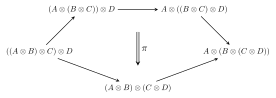
\includegraphics{figures/c7-fig06.svg}\end{equation}


The so-defined pentagrammator must itself satisfy some compatibility
conditions. Not surprisingly, it comes from a cell of dimension 3 in Stasheff's
associahedron $K_5$ (see \reref{r:stasheff}). Recall that  this polyhedron has
14 vertices, corresponding to 14 bracketings of the tensor product of 5
objects; edges of $K_5$  correspond to application of associativity
isomorphisms, and 2-cells correspond to  pentagon axiom and functoriality
relation. As discussed before, the MacLane coherence axiom for monoidal
categoires implies that the 2-skeleton of $K_5$ is simply-connected.  In fact,
it is homeomorphic to a 2-sphere: $K_5$ is topologically a 3-ball, and the
2-skeleton is the boundary of that ball.

We now add a relation corresponding to the single 3-cell in $K_5$;
this relation has the form
\begin{align*}
  &\text{(composition
  of 2-morphisms in the 2-cells in the upper hemisphere)}\\
  & \qquad =
  \text{(composition of 2-morphisms in the 2-cells in the lower hemisphere)}.
\end{align*}

This gives us a consistency relation for the pentagrammator 2-morphism, called
the \emph{associahedron} equation. To give you some idea of what it looks like,
\firef{f: associahedron} shows the pasting diagram for one side of the
associahedron equation, which corresponds to the upper hemisphere in the
14-vertex 3-cell. The lower side is similar. (This diagram is copied from
\cite[Appendix C]{schommer-pries}; he uses $a$ instead of $\al$ for the
associativity 1-morphism.)

\begin{figure}[ht]
\tikzset{l/.style={font=\fontsize{8}{8}\selectfont}}
   \begin{center}
       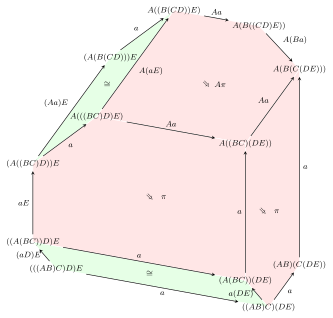
\includegraphics{figures/c7-fig07.svg}% End sketch output
	\end{center}
	\caption{Pasting diagram for the left-hand side of the associahedron axiom.
    Green 2-cells correspond to commutative diagrams given by functoriality.}
	\label{f: associahedron}
\end{figure}

In a similar way, instead of requiring the commutativity of diagrams involving
the left and right unit isomorphisms, we now need to introduce 2-morphisms
(``unitors'') filling these diagrams, and then impose additional relations on
them coming from 3-cells.

We will not be providing any details of this, referring the reader to
\cite{schommer-pries}. Instead, we will show some examples.


\begin{example}\label{x:alg-bimodules}
  Let $\Alg$ be the weak 2-category of algebras and bimodules as defined in
  \exref{x:alg}. Then it has a natural structure of a symmetric monoidal
  2-category, with $\otimes$ being the usual tensor product of algebras.
\end{example}

\begin{remark}
  Recall that a monoidal category $\calC$ is essentially the same as a
  weak 2-category $\calB\calC$ with one object. Similarly, a monoidal
  2-category is the same as a weak 3-category with one object; the
  associahedron equation is a special case of a consistency equation for
  associativity of composition of 1-morphisms in a 3-category.
\end{remark}


%%%%%%%%%%%%%%%%%%%%%%%%%%%%%%%
\section{Locally finite categories and Deligne product}
\label{s:deligne-product}
In this section, we give an example of a symmetric monoidal weak 2-category.
Namely, recall that a $\kk$-linear abelian category $\calA$ is called
\emph{locally finite}\index{category!locally finite} if
\begin{itemize}
    \item for any $X,Y\in \calA$, the space $\Hom_{\calA}(X,Y)$ is
      finite-dimensional, and
    \item every object $X\in \calA$ has finite length
\end{itemize}
(see \cite[Section 1.8]{etingof-fusion}). Denote by $\Linlf$ the 2-category
of locally finite $\kk$-linear abelian categories, with 1-morphisms given by
\emph{right exact} $\kk$-linear functors and 2-morphisms given by functorial
morphisms (some motivations for restricting ourselves to right exact
functors will be discussed in \chref{c:3cat-tens}). %FIXME


Our next goal is defining an analog of tensor product in $\Linlf$.
Let $\calC, \calD, \calE$ be $\kk$-linear categories. Denote by
$\Bil(\calC\times\calD, \calE)$ the category of $\kk$-bilinear functors $F\colon
\calC\times\calD\to \calE$ which are right exact in each of the arguments.

\begin{definition}\label{d:deligne-product}
  The Deligne product of $\kk$-linear categories $\calC$, $\calD$ is a
  $\kk$-linear category $\calC\boxtimes \calD$ together with a bilinear functor
  $\calC\times\calD\to \calC\boxtimes\calD$ such that for any $\calE$, we have
  an equivalence
  $$
    \Bil(\calC\times\calD, \calE)\simeq \Fun(\calC\boxtimes\calD, \calE).
  $$
  where $\Fun$ is the category of $\kk$-linear right exact functors.
\end{definition}
This definition mimics the definition of tensor product of vector spaces as a
universal object. As usual with such definitions, if such a category
$\calC\boxtimes\calD$ exists, it is unique: any two such categories are
canonically equivalent. However, existence is not obvious and in fact may fail
without some assumptions on $\calC$, $\calD$.

\begin{theorem}\label{t:deligne-product}\index{Deligne's product}
  If $\calC$, $\calD$ are locally finite categories,
  then $\calC\boxtimes \calD$ exists
  and is a locally finite $\kk$-linear category.
\end{theorem}
We refer the reader to \cite[Section 1.11]{etingof-fusion} for the proof of
this theorem as well as results below.
\begin{lemma}\label{l:deligne-product-mod}
  \begin{enumerate}
  \item
    For a finite-dimensional algebra $A$, denote by $A\mod$ the category of
    finite-dimensional left $A$-modules. Then
    $$
      (A\mod)\boxtimes (B\mod) \simeq (A\otimes B)\mod.
    $$
  \item
    For any objects $X_1, Y_1\in \calC$, $X_2, Y_2\in \calD$, we have a
    canonical isomorphism
    $$
       \Hom_{\calC \boxtimes \calD} (X_1\boxtimes X_2, Y_1\boxtimes Y_2 )\simeq
         \Hom_{\calC} (X_1,  Y_1) \otimes
         \Hom_{\calD} (X_2, Y_2 ).
    $$
  \item If $\calC$, $\calD$ are semisimple $\kk$-linear categories with simple
    objects $X_i, Y_j$ respectively, then $\calC\boxtimes \calD$ is also
    semisimple, with simple objects $X_i\boxtimes Y_j$.
   \end{enumerate}
\end{lemma}

\begin{theorem}\label{t:linear-monoidal-2cat}
  The 2-category $\Linlf$ is a symmetric monoidal 2-category, with tensor
  product functor given by Deligne's product $\boxtimes$ and unit given by the
  category $\vecf$.
\end{theorem}
We skip the proof, which is mostly straightforward; we just note that to show
that $\vecf$ is the unit for this monoidal structure, we need to construct,
for any $\calC\in \Linlf$, an equivalence of categories $\vecf\boxtimes
\calC\simeq \calC$.

Another way of stating this is by saying that any locally finite $\kk$-linear
category has a natural structure of a module category over $\vecf$ (we will
discuss the general notion of a module category later, in
\seref{s:module-categories}). Namely, for a
finite-dimensional vector space $V$ and an object $X\in \calC$ in a locally
finite category $\calC$, we define the object $V\otimes X$ by the condition that
for any object $Y\in \calC$, we have a canonical isomorphism
$$
  \Hom(Y, V\otimes X)=V\otimes \Hom(Y, X)
$$
(more formally, $V\otimes X$ is the object (co)representing the functor
$F(Y)=V\otimes \Hom(Y,X)$).

\clearpage

%!TEX root = TQFTnotes.tex
%%%%%%%%%%%%%%%
\chapter{Duality in 2-categories}\label{c:duality-2cat}

Recall that for an object $X$ in a monoidal category, we have defined the
notion of left and right duals. We will now extend this notion to objects and
1-morphisms in a weak 2-category $\calC$. Doing it for objects requires
defining a monoidal structure on $\calC$; duality for 1-morphisms (also known as
adjunction) can be defined in any 2-category.

Throughout this section $\calC$ is a weak 2-category.
%%%%%%%%%%%%%%%%%%%%%%%%%%%%%%%%
\section{Adjunction for 1-morphisms}\label{s:adjunction}
\begin{definition}\label{d:adjunction}\index{adjunction!in 2-category}
  Let $\calC$ be a weak 2-category. An \emph{adjunction} in $\calC$ is the
  following data:
  \begin{itemize}
    \item A pair of 1-morphisms $f\in\Hom(X,Y)$, $g\in \Hom(Y,X)$
    \item A 2-morphism $\eta\colon 1_X\to g\circ f$ (unit of adjunction)
    \item A 2-morphism $\eps\colon f\circ g\to 1_Y$ (counit of adjunction)
  \end{itemize}
  satisfying the adjunction equations:
  \begin{equation}\label{e:adjunction}
    \begin{aligned}
      &(f\xto{} f \circ 1_X \xto{1_f\circ \eta}
        f\circ g\circ f \xto{\eps \circ 1}
        f\circ 1_Y \xto{} f)=1_f\\
      &(g\xto{}  1_X \circ g \xto{\eta\circ 1_g}
        g\circ f\circ g \xto{1 \circ \eps}
        1_X\circ g \xto{} g)=1_g
    \end{aligned}
  \end{equation}

  In this situation, we say that $f$ is the \emph{left
  adjoint}\index{adjoint!left} of $g$ and $g$ is the \emph{right
  adjoint}\index{adjoint!right} of $f$; we will write $$
  X\xrightleftharpoons[g]{f}Y. $$ Alternative notation for adjunction is
  $f\dashv g$; in both notations, the unit and the counit 2-morphisms are
  implicit.
\end{definition}

To understand the adjunction equations, we can use pasting diagrams to describe
the 2-morphisms in the left-hand side of these equations:

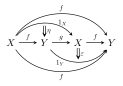
\includegraphics{figures/c8-fig01.svg}
\qquad
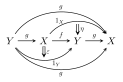
\includegraphics{figures/c8-fig02.svg}


Alternatively --- and more intuitively --- we can use string diagrams.
Namely, we will illustrate 2-morphisms $\eta$ and $\eps$ by string diagrams as
in \firef{f:adjunction_units}. Then the adjunction equations become the
equations of \firef{f:AdjunctionStringDiagram}, justifying our choice of
graphical depiction.
\begin{figure}[ht]
  \begin{center}
    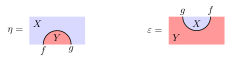
\includegraphics{figures/c8-fig03.svg}
    \caption{String diagrams for adjunction unit and counit.}
    \label{f:adjunction_units}
  \end{center}
\end{figure}

\begin{figure}[ht]
  \begin{center}
    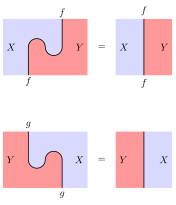
\includegraphics{figures/c8-fig04.svg}
    \caption{Adjunction equations via string diagrams}
    \label{f:AdjunctionStringDiagram}
  \end{center}
\end{figure}

The definition of adjunction given above generalizes two well-known examples:
duality in a monoidal category and adjunction of functors.

\begin{example}\label{x:adjunction-monoidal}
  Let $\calC$ be a monoidal category, and let $B\calC$ be the corresponding
  2-category with one object as defined in \exref{x:BC}. Then the definition of
  adjunction for 1-morphisms in $B\calC$ coincides with the notion of dual pairs
  of objects in $\calC$: $A\dashv B$ as 1-morphisms in $B\calC$ if and only if
  $B$ is the right dual of $A$ in $\calC$.
\end{example}

\begin{theorem}\label{t:adjunction-cat}\index{adjunction!for functors}
  Let $\cat$ be the 2-category of small categories. Let $f\colon \calC\to
  \calD$, $g\colon \calD\to \calC$ be 1-morphisms in $\cat$ \textup{(}i.e., functors
  between the corresponding categories\textup{)}. Then defining adjunction data
  $\eta, \eps$ as in \deref{d:adjunction} is equivalent to defining
  a functorial isomorphism
  \begin{equation}\label{e:adjunction-cat}
    \Hom_{\calD}(f(-), -)\simeq \Hom_{\calC}(-, g(-)).
  \end{equation}
\end{theorem}
\begin{proof}
  (Sketch of proof)

  Suppose we are given a functorial isomorphism \eqref{e:adjunction-cat}. Then
  for any object $c\in \calC$, we have isomorphism $\Hom_{\calD}(f(c),
  f(c))\simeq \Hom_{\calC}(c, g(f(c)))$. In particular, applying it to the
  identity morphism $1_{f(c)}$, we get a canonical element $\eta\in \Hom(c,
  g(f(c)))$, or equivalently, a functorial morphism $\id_{\calC}\to g\circ f$,
  which can be used as the unit of adjunction as in \deref{d:adjunction}.
  Similarly we get a functorial morphism $\eps\colon fg(d)\to d$, which is the
  counit of adjunction. The adjunction relations shown in
  \firef{f:AdjunctionStringDiagram} follow from the functoriality of
  \eqref{e:adjunction-cat}.

  We leave the construction in the opposite direction as an exercise to the
  reader.

\end{proof}

Adjoint functors between categories frequently appear as
``restriction--induction'' pairs; we give several examples below.
\begin{example}\label{x:coset-bimodule}
  Let $G$ be a finite group and $H\subset G$ a subgroup. Consider the
  restriction functor $\Res\colon \Rep G\to \Rep H$. Then it has a left adjoint
  called the induction functor $\Ind \colon \Rep H\to \Rep G$. The adjunction
  relation
  $$
  \Hom_G(\Ind V, W)\simeq \Hom_H(V, \Res W), \qquad V\in \Rep H, W\in \Rep G
  $$
  is known as \emph{Frobenius reciprocity}\index{Frobenius reciprocity};
  from our point of view, it is the
  definition of the induction functor.
 \end{example}

\begin{example}\label{x:abelian-groups-duality}
  Let $\calC$ be the category of abelian groups. It has an obvious forgetful
  functor $F\colon \calC\to\sets$. This functor has a left adjoint
  $I\colon\sets\to \calC$; namely, $I(S)$ is the abelian group freely generated
  by elements of $S$. Again, we take it as the definition of ``freely
  generated''; the nontrivial fact is that such a left adjoint exists.
\end{example}


Returning to adjunction in an arbitrary 2-category $\calC$,
here are some useful results about adjunctions.

\begin{lemma}\label{l:adjunction-unique}
  Let $f\colon X\to Y$ be a 1-morphism in a weak 2-category $\calC$. Then
  the remaining adjunction data, $g, \eta, \eps$ \textup{(}as in
  \deref{d:adjunction}\textup{)}, if it exists, is unique up to unique isomorphism: if
  $(f,g,\eta,\eps)$ and $(f, \tilde g, \tilde \eta, \tilde \eps)$ are two
  different sets of adjunction data with the same $f$, then there is a
  unique 2-morphism $\al\colon g\to \tilde g$ which makes the appropriate
  diagrams commutative.
\end{lemma}
We leave the proof as an exercise (see also \cite[Section IV.1]{mac-lane}).

A variation of this is the following result.
\begin{lemma}\label{l:adjunction-unique2}
  The unit of the adjunction is uniquely determined by the remaining
  adjunction data: if $(f, g, \eta, \eps)$ and $(f, g, \eta', \eps)$ are two
  sets of adjunction data, then
  $\eta=\eta'$.

  Similarly, the counit $\eps$ of adjunction is uniquely determined by
  $(f,g, \eta)$.

  Moreover, if $(f, g, \eta, \eps)$ satisfies one of the adjunction equations
  \eqref{e:adjunction}, and $(f, g, \eta', \eps)$ satisfies the other one,
  then $\eta=\eta'$ \textup{(}and thus satisfies both equations\textup{)}.
\end{lemma}
\leref{l:adjunction-unique} and \leref{l:adjunction-unique2} are analogs of
\thref{t:dual_unique1} and \ecref{ec:coev-unique} for monoidal categories,
and the proofs are similar (see \cite[Lemma 2.3.8]{lurie-cobordism}).



The notion of adjunction is closely related to the notion of equivalence. Recall
that a 1-morphism $f\colon X\to Y$ in a 2-category is called an
\emph{equivalence}\index{equivalence!of 1-morphisms} if there exists $g\colon
Y\to X$ such that $fg\simeq 1_Y$, $gf\simeq 1_X$. (This is a weaker version of
an invertible morphism --- requiring that $fg=1_Y$ would be too strict, since
1-morphisms in a 2-category are usually only isomorphic, not equal.)

\begin{lemma}\label{l:adjoint-equivalence}
  If $f\colon X\to Y$, $g\colon Y\to X$ are 1-morphisms in a weak
  2-category such that $fg\simeq 1_Y$, $gf\simeq 1_X$, then
  $g$ is both a left and a right adjoint of $f$.
\end{lemma}
\begin{proof}
  Choose arbitrary isomorphisms $\al\colon fg\isoto 1_Y$, $\be \colon gf\isoto
  1_X$. Then the composition
  $$
  \theta = (f\xto{ \al^{-1} \ccirc 1_f} fgf\xto{1_f\ccirc \be} f)
  $$
  is an invertible 2-morphism $f\to f$. Thus, setting $\eta = (\theta^{-1}\ccirc
  1_g) \al^{-1}$, $\eps = \be$ we see that the so-defined $\eta, \eps$ satisfy one
  of the adjunction equations. In a similar way we can find $\eta', \eps$ which
  satisfy the other adjunction equation. Now the result follows from
  \leref{l:adjunction-unique2}.
\end{proof}
In other words, every equivalence can be upgraded to an adjoint equivalence.



%In a monoidal category, given an object $B$ which has a left dual $B^*$,
%we have functorial isomiorphisms
%$$
%\Hom (A\otimes B, C)\simeq \Hom(A, C\otimes B^*)
%$$
%given by the picture below.
%
%A similar statement holds in a weak 2-category: we have a bijection
%$$
%\Hom(f \circ g,h )\simeq \Hom(f, h\circ g^*)
%$$
%where $g^*$ is right adjoint of $g$.
%
%FIXME

%%%%%%%%%%%%%%%%%%%%%%%%%%%%%%%%%%%%%%%%%%%%%%%%%%%%%%%%%%%%%%%%%%%%%%%%
\section{Dual objects in 2-categories}\label{s:coherent-dual-pair}

Let us now talk about dual objects in $\calC$. It only makes sense
if $\calC$ has a monoidal structure; thus, in this section we assume that
$\calC$ is a monoidal weak 2-category.

Recall that in a (usual) monoidal category, we defined a dual pair as the data
$(A,B, \ev, \coev)$, where $\ev\colon A\otimes B\to \one$,
$\coev \colon \one \to B\otimes A$ are morphisms satisfying the zigzag (or
rigidity) relations $z_A= 1_A$, $z_B = 1_B$, where
\begin{equation}\label{e:zigzags}
    \begin{aligned}
        z_A&= (A\xto{1_A\otimes \coev} A\otimes B \otimes A \xto{\ev\otimes
        1_A} A)\\
        z_B &= (B \xto{\coev \otimes 1_B} B\otimes A \otimes B
        \xto{1_B\otimes\ev} B)
\end{aligned}
\end{equation}
(see \deref{d:dual-object}).

We now want to upgrade this definition, defining the notion of a dual pair in a
monoidal weak 2-category. In this case, it makes no sense to require $z_A=1_A$,
$z_B=1_B$; instead, we need isomorphisms $\al \colon z_A\to 1_A$, $\be\colon
z_B\to 1_B$. Moreover, it is natural to expect that these isomorphisms
themselves should satisfy some compatibility relations. Following
\cite{pstragowski}, we will impose the following relations.

Let $zz_+$ be the ``double zigzag'' 1-morphism
\begin{equation}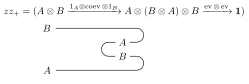
\includegraphics{figures/c8-eqfig01.svg}\end{equation}
(we have turned the picture 90 degrees counterclockwise, to match our
convention that in 2-categories, 1-morphisms go ``from left to right'').

Then we have two different 2-morphisms $zz_+\to \ev$: $\al\otimes 1$, obtained
by using $\al$ on the lower part of zigzag, and $1\otimes \be$, obtained by using
$\be$ on the top part of zigzag (we leave it to the reader to write them
algebraically).

It is natural to require that these 2-morphisms are equal:
\begin{equation}\label{e:swallowtail1}
\includegraphics{figures/c8-fig05.svg}\end{equation}
Similarly, we can define a 1-morphism $zz_-\colon \one\to B\otimes A$ by the
picture below
\begin{center}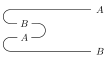
\includegraphics{figures/c8-eqfig02.svg}\end{center}
As with $zz_+$, there are two different 2-morphisms $zz_-\to \coev$, and we
require that they
are equal:
\begin{equation}\label{e:swallowtail2}
\includegraphics{figures/c8-fig06.svg}\end{equation}
We will call relations \eqref{e:swallowtail1}, \eqref{e:swallowtail2}
\emph{swallowtail relations}\index{swallowtail relations}.
The name comes from their geometric interpretation
in terms of 2-cobordisms, which we will discuss in the next section.

Thus, we are led to the following definition (we use the terminology of
\cite{pstragowski}).

\begin{definition}\label{d:coherent-dual-pair}\index{dual pair!in 2-category}
  A \emph{coherent dual pair} in a weak monoidal 2-category
  $\calC$ is the following collection of
  data:
  \begin{itemize}
    \item Objects $A, B\in \calC$.
    \item 1-morphisms $\ev  \colon A\otimes B\to \one$,
      $\coev \colon \one \to B\otimes A$.
    \item Invertible 2-morphisms $\al \colon z_A\to 1_{A}$,
      $\be \colon z_B\to 1_{B}$, where $z_A$, $z_B$ are defined
      by \eqref{e:zigzags}.
  \end{itemize}
  such that $\al, \be$ satisfy the swallowtail relations
  \eqref{e:swallowtail1}, \eqref{e:swallowtail2}.

  In this case, we say that $B$ is a right dual of $A$, and $A$ is a left
  dual of $B$.
\end{definition}


\begin{lemma}\label{l:dual-pair-upgrade}
  Let $(A, B, \ev, \coev, \al, \be)$ be as in the definition of
  coherent dual pair, but without the swallowtail relations.
  Then one can replace $\be$ by another
  2-isomorphism $\tilde \be$ so that
  $(A, B, \ev, \coev, \al, \tilde \be)$ is a coherent dual pair.
\end{lemma}

In other words, if you have any isomorphisms $z_A\to 1_A$, $z_B\to 1_B$,
then you can modify one of them to satisfy the swallowtail relations.

The proof of this lemma is similar to \leref{l:adjoint-equivalence}, where
we also argued that given a pair of isomorphisms, we can modify one of them
to satisfy an additional consistency requirement (in that case, the adjunction
property). We refer the reader to \cite[Theorem 2.7]{pstragowski} for
details of the proof.

Recall that for a weak 2-category $\calC$, we defined a (usual) category
$h\calC$ by making 1-morphisms that were isomorphic in $\calC$ equal in
$h\calC$, see \deref{d:hC}. Then \leref{l:dual-pair-upgrade} implies that
any dual pair $(A,B, \ev, \coev)$ in $h\calC$ can be ``upgraded'' to a
coherent dual pair in $\calC$. In particular, this implies the following.

\begin{corollary}\label{c:dual-objects-2cat}
  An object $A\in \calC$ has a right \textup{(}respectively, left\textup{)} dual in $\calC$
  if and only if it has the right \textup{(}respectively, left\textup{)}
  dual in the homotopy category $h\calC$.
\end{corollary}

We can also ask whether, for a given $A$, all coherent dual pairs
including it are equivalent. To do that, we define the notion of
an isomorphism of dual pairs, which consists of a pair of isomorphisms of
objects and 2-isomorphisms between evaluation and coevaluation; details
can be found in \cite[Section 2.2]{pstragowski}.


\begin{theorem}\label{t:coh-dual-pair-unique}
    Let $A$ be an object in $\calC$, and let $(A,B, \dots)$,
    $(A, B', \dots)$ be two coherent dual pairs including $A$.
    Then there exists an isomorphism between them which is identity on $A$.
\end{theorem}

(This is a simplified version; a more accurate statement, which also
answers the question of whether such an isomorphism is unique, is given
in \cite[Theorem 2.14]{pstragowski} and says that the 2-groupoid of
coherent dual pairs is equivalent to the 2-groupoid of
objects in $\calC$ which have a right dual.)

In summary, we see that any dual pair in $h\calC$ can be ``upgraded'' to a
coherent dual pair in $\calC$, and any two such upgrades are isomorphic. Thus,
producing such a coherent dual pair is essentially equivalent to producing an
object $A\in \calC$ which has a right dual in $h\calC$.


\begin{remark}
  In all our discussions in this section, we ignored associativity and unit
  isomorphisms in the monoidal 2-category $\calC$. Technically speaking,
  this is not correct, and we must include them. Unfortunately, if we do
  that, all diagrams become hopelessly complicated --- for example, here is
  the diagram of one of the swallowtail relations in all glorious detail, taken
  from \cite{pstragowski}:

  
\includegraphics[width = 0.8\textwidth]{swallowtail.pdf}
\end{remark}


Finally, we give the following definitions.

\begin{definition}\label{d:category-duals}\index{category!with duals}
  A symmetric monoidal weak 2-category $\calC$ is called a \emph{category with
  duals} if
  \begin{enumerate}
    \item Every object $A\in \calC$ is rigid, i.e., has a dual in $\calC$.
    \item Every 1-morphism has both left and right adjoints.
  \end{enumerate}
\end{definition}

\begin{definition}\label{d:fully-dualizable-2cat}\index{fully dualizable object}
  An object $A$ in a symmetric monoidal weak 2-category $\calC$ is called
  \emph{fully dualizable} if it lies in some subcategory $\calD\subset
  \calC$ which is a category with duals.
\end{definition}

It is not difficult to show (see \cite[Proposition
  4.2.3]{lurie-cobordism}) that an object $A$ is fully dualizable if and only if $A$ has a
dual $A^*$ and the corresponding evaluation and coevaluation 1-morphisms
have left and right adjoints. Moreover, the existence of adjoints for $\ev$
implies the existence of adjoints for $\coev$ and vice versa.

%%%%%%%%%%%%%%%%%%%%%%%%%%%%%%%
\section{Serre functor}\label{s:serre}
Let $\calC$ be a symmetric monoidal 2-category, and let $A$ be a fully
dualizable object in $\calC$. Denote by $B=A^*$ the dual of $A$ and by
$\ev\colon A\otimes B\to \one$, $\coev\colon \one \to B\otimes A$ the
corresponding evaluation and coevaluation morphisms.

By the definition of a fully dualizable object, the morphism $\ev$ must have right and
left adjoints, which we will denote by $\ev^R$, $\ev^L$ respectively. Both of
them are morphisms $\one \to A\otimes B$; thus, we have adjunctions
\begin{align*}
&A\otimes B \xrightleftharpoons[\ev^R]{\ev}\one,\\
&\one \xrightleftharpoons[\ev]{\ev^L}A \otimes B.
\end{align*}

It is natural to ask what is the relation between these adjoints and the
coevaluation morphism $\coev\colon \one \to B \otimes A$. Note that here $A$ and
$B$ go in the opposite order, but since $\calC$ is a symmetric monoidal
category, we can use the commutativity isomorphism to exchange them, defining
$\widetilde\coev = c_{B,A}\coev\colon \one \to A\otimes B$. It turns out that
while in general, $\widetilde\coev$ is different from $\ev^L$, $\ev^R$, they can
be related using the so-called \emph{Serre automorphism}.

\begin{definition}\label{d:serre}\index{Serre automorphism}
  Let $A$ be a fully dualizable object in $\calC$. The Serre morphism $S_A$ is the
  1-morphism $A\to A$ defined by
  \begin{equation}\label{e:serre-formula}
    S_A=\Bigl(
     A\xto{1_A\otimes \ev^R} A\otimes A\otimes B \xto{c_{A,A}\otimes 1_B}
     A\otimes A\otimes B \xto{1_A\otimes \ev} A
         \Bigr).
   \end{equation}
   Graphically, this composition is represented by the picture
   \eqref{e:serre-picture} below:
   \begin{equation}\label{e:serre-picture}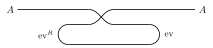
\includegraphics{figures/c8-fig07.svg}\end{equation}
   where the input/output of $S_A$ are the two horizontal strands labeled $A$,
   and the loop formed by $\ev^R$ and $\ev$ represents the auxiliary
   $A\otimes B$ pair created and then annihilated; the crossing in the middle
   is the symmetry isomorphism $c_{A,A}$.
\end{definition}

\begin{remark}
  The name ``Serre automorphism'' is motivated by the relation of this to Serre
  duality in the category of coherent sheaves on projective varieties; see
  \cite[Remark 4.2.4]{lurie-cobordism}.
\end{remark}


\begin{theorem}\label{t:serre}
  Let $A$ be a fully dualizable object in $\calC$ and let
  $S_A\colon A\to A$ be the Serre morphism defined by \deref{d:serre}.
   Then $S_A$ is invertible, and we have an isomorphism of 1-morphisms
   \begin{align*}
   \ev^L&\simeq (S\otimes 1_B)  \widetilde \coev \\
   \ev^R&\simeq (S^{-1}\otimes 1_B)\widetilde \coev.
   \end{align*}
\end{theorem}
We refer the reader to \cite[Section 3.1]{pstragowski} for the proof.

In particular, this theorem implies that if the Serre automorphism is trivial
(i.e., one has a 2-isomorphism $S_A\simeq 1_A$), then $\ev, \widetilde\coev$ are
two-sided adjoints of each other. More precisely, a choice of an isomorphism
$S_A\simeq 1_A$ defines the unit and counit of adjunctions $\ev\dashv
\widetilde\coev$, $\widetilde\coev\dashv\ev$.



%%%%%%%%%%%%%%%%%%%%%%%%%%%%%%%
\section{Duality in $\Linlf$}\label{s:lin-duals}
As the simplest example of duality in a 2-category, let us consider the
2-category $\Linlf$ of locally finite $\kk$-linear  categories, introduced in
\seref{s:deligne-product}. Recall that objects of that category are $\kk$-linear
abelian categories such that all $\Hom$ spaces are finite-dimensional and every
object has finite length. This 2-category has a natural symmetric monoidal
structure, given by Deligne's product $\boxtimes$.

Let us now analyze which objects of $\Linlf$ are rigid, i.e., for which
categories $\calC$ there exist a category $\calD$ and functors
\begin{align*}
  \eta&\colon \vecf \to \calD\boxtimes \calC\\
  \epsilon&\colon \calC\boxtimes \calD\to \vecf
\end{align*}
satisfying the rigidity axioms. Clearly, defining the functor $\eta$ is equivalent
to choosing an object
$$
  e=\eta (\kk)=\bigoplus_{i=1}^k Y_i\boxtimes X_i\in \calD\boxtimes \calC
$$
together with functorial isomorphisms
\begin{equation}\label{e:rigidity-lin}
  \begin{aligned}
    X&\simeq \bigoplus \eps(X,Y_i)\otimes X_i\\
    Y&\simeq \bigoplus \eps(X_i,Y)\otimes Y_i
  \end{aligned}
\end{equation}
for every $X\in \calC$, $Y\in \calD$.

\begin{theorem}\label{t:dualizable-linear}
  Let $\kk$ be an algebraically closed field of characteristic zero. Then a
  category $\calC\in \Linlf$ is rigid as an object of $\Linlf$ if and only if it
  is semisimple and has finitely many isomorphism classes of simple objects. In
  this case, the dual category $\calD$ is equivalent to the category of
  $\kk$-linear functors $\calC\to \vecf$; under this equivalence, the counit
  $\eps\colon \calC\boxtimes\calD\to \vecf$ is given by
  $$
    \eps(X,F) = F(X)\in \vecf,\qquad X\in \calC, F\in \Fun(\calC, \vecf)
  $$
  and the object $e=\bigoplus Y_i\boxtimes X_i$ is given by
  $$
    e=\bigoplus X^i \boxtimes X_i
  $$
  where the sum is over isomorphism classes of simple objects $X_i\in \calC$,
  and for such a simple object, we define
  $$
    X^i=\Hom(X_i, -)\in \Fun(\calC, \vecf).
  $$
\end{theorem}
\begin{proof}
  Our proof follows \cite[Section A.6]{bdspv}, where the proof is attributed
  to Andr\'e Henriques. (Note that they work in greater generality: they do not
  require the category to be abelian, instead imposing a weaker condition of
  Cauchy completeness.)


  First, finiteness easily follows from the observation that by
  \eqref{e:rigidity-lin}, any $X\in \calC$ is a subobject in a finite direct sum
  of copies of $X_1, \dots, X_k$. Thus, the only simple objects that can appear
  in the Jordan--H\"older series for $X$ are those simple objects that appear in
  the Jordan--H\"older series for one of the $X_i$; which implies that there are only
  finitely many of them.

  To prove semisimplicity, let $0\to A_1\to A_2\to A_3\to 0$ be a short exact
  sequence in $\calC$. Using \eqref{e:rigidity-lin}, we can rewrite it as a
  short exact sequence
  $$
  0 \to \bigoplus \eps(Y_i, A_1)\otimes X_i
    \to \bigoplus \eps(Y_i, A_2)\otimes X_i
    \to \bigoplus \eps(Y_i, A_3)\otimes X_i
  \to 0.
  $$
  Since a direct sum of complexes is exact if and only if each summand is
  exact, this implies that each complex
  $$
  K_i = \Bigl(
      0 \to  \eps(Y_i, A_1)\otimes X_i
          \to  \eps(Y_i, A_2)\otimes X_i
          \to \eps(Y_i, A_3)\otimes X_i
        \to 0
        \Bigr)
  $$
  is exact. This in turn is equivalent to the requirement that the complex of
  vector spaces
  $$
    0 \to  \eps(Y_i, A_1)
            \to  \eps(Y_i, A_2)
            \to \eps(Y_i, A_3)
    \to 0
  $$
  is exact. But each short exact sequence of vector spaces splits; thus, each
  short exact sequence $K_i$ splits, which implies that the original short
  exact sequence $0\to A_1\to A_2\to A_3\to 0$ also splits. Thus, $\calC$ is
  semisimple.

  We leave the proof of the remaining parts of the theorem as an exercise to the
  reader.
 \end{proof}

 After establishing duality for objects of $\Linlf$, we can turn to establishing
 duality for 1-morphisms. For simplicity, we give the answer for a slightly
 smaller 2-category of \emph{finite} $\kk$-linear categories.

 \begin{definition}\label{d:finite}
    A locally finite $\kk$-linear category $\calA$ is called \emph{finite}\index{category!finite} if
    it satisfies the following additional conditions
    \begin{itemize}
      \item The set of isomorphism classes of simple objects in $\calA$ is
        finite.
      \item There are enough projective objects.
    \end{itemize}
\end{definition}
A more detailed discussion of finite categories can be found, e.g., in
\cite[Section 1.8]{etingof-fusion}.

 \begin{theorem}\label{t:exact-adjoint}
  Assume that $\kk$ is an algebraically closed field of characteristic zero. Let
  $\calC$, $\calD\in \Linlf$ be finite $\kk$-linear categories. Then a functor
  $F\colon \calC\to \calD$ has a left adjoint if and only if it is left exact.
\end{theorem}
A proof of this theorem can be found in \cite[Proposition 1.7]{dsps-balanced}
(strangely enough, even though the result was part of folklore for years, it was
not written down prior to this paper).

\begin{corollary}\label{c:adjoint-semisimple}
  Let $\calC, \calD$ be finite semisimple categories. Then any functor $F\colon
  \calC\to \calD$ admits both left and right adjoints.
\end{corollary}

\begin{exercise}\label{ec:adjoint-semisimple}
  Under the assumptions of \coref{c:adjoint-semisimple}, let $X_i$, $i=1, \dots,
  n$ be simple objects of $\calC$ and $Y_j, j=1, \dots, m$ be simple objects of
  $\calD$.

  \begin{enumerate}
    \item Show that the category of functors $\Fun(\calC, \calD)$ is naturally
      equivalent to the category whose objects are $m\times n$ matrices of
    finite-dimensional vector spaces. (Hint: it suffices to consider functors
    $\vecf\to \vecf$).

    \item Show that the (two-sided) adjoint of such a matrix of vector spaces is
    the matrix obtained by transposing the original matrix and replacing each
    vector space by the dual.
  \end{enumerate}
\end{exercise}

Combining \thref{t:dualizable-linear} with \coref{c:adjoint-semisimple}, we get
the following result.

\begin{theorem}\label{t:fd-linear}
   Assume that $\kk$ is an algebraically closed field of characteristic zero.
   Then fully dualizable objects in $\Linlf$ are finite semisimple
   $\kk$-linear categories.
\end{theorem}




\clearpage

\include{c9-separable-src-gerby}
\include{c10-2d-extended-src-gerby}
\include{c11-PL-src-gerby}
%!TEX root = TQFTbook.tex
%%%%%%%%%%%%%%
\chapter{Lattice construction of extended 2d TQFT}\label{c:2d-lattice}

In this chapter, we give an alternative approach to constructing 2d TQFT, based
on triangulating a manifold (or, more generally, choosing a PLCW decomposition,
as described in the previous chapter). In this approach, an invariant of a
closed 2-manifold is defined by a suitable sum over all ways of ``coloring''
cells of a given PLCW decomposition (we will explain it in more detail below).
In physics, such a sum is usually referred to as ``state sum''; it should be
considered a discretized analog of the path integral.

In the special case of DW theory, this approach is known as ``lattice gauge
theory'' and has been extensively studied by physicists. Generalization of
this to an arbitrary separable symmetric Frobenius algebra was suggested in
\cite{fhk}. See also \cite{oeckl}. Generalization to arbitrary symmetric
monoidal 2-categories is discussed in \cite{davidovich}.

Throughout this chapter, we fix a separable symmetric Frobenius algebra
$A$. As before, we assume that the ground field $\kk$ has characteristic 0.
We denote by $\eps \colon A\to \kk$ the counit. We also denote by
$(a,b)=\eps(ab)$ the corresponding bilinear pairing.
\section{Definition of TQFT via state sum}\label{s:state-sum}
As before, let $x_i$, $x^i$ be dual bases in $A$ with respect to the
Frobenius pairing. We denote by $g_{ij}$ the matrix of the pairing in
the basis $x_i$: $g_{ij}=(x_i,x_j)$ and by $g^{ij}$ the inverse matrix:
$\sum_{j} g_{ij}g^{jk}=\de_{ik}$. We will use $g_{ij}$, $g^{ij}$ for
raising and lowering indices of various tensors.

For any $k \ge 0$, define the map $A^k\to \kk$ by
\begin{equation}\label{e:k-pairing}
\< a_1, \dots, a_k\> = \eps (a_1\cdot \dots \cdot a_k).
\end{equation}

\begin{lemma}\label{l:k-pairing}
  \par\noindent
  \begin{enumerate}
    \item The map \eqref{e:k-pairing} is invariant under cyclic permutation of
      $a_i$:
      $$
      \< a_1, \dots, a_k\> = \<a_k, a_1, \dots, a_{k-1}\>.
      $$
    \item The map \eqref{e:k-pairing} is multilinear over $\kk$. Moreover, it is
      linear over $A$: for any $i=1,\dots, k$, $x\in A$, we have
      $$
        \< a_1, \dots, a_ix, a_{i+1},\dots, a_k\> =
        \< a_1, \dots, a_i, xa_{i+1},\dots, a_k\>
      $$
      \textup{(}for $i=k$, we take $a_{i+1}=a_1$\textup{)}.
    \item
      \begin{equation}\label{e:k-pairing-2}
        \sum_i \< a_1, \dots, a_k, x_i\> \< x^i, b_1, \dots, b_m\>
         =\< a_1, \dots, a_k, b_1, \dots, b_m\>
      \end{equation}
  \end{enumerate}
\end{lemma}
The proof of this lemma is straightforward and is left as an exercise to
the reader.

Let $M$ be a closed oriented 2-dimensional manifold. Let us choose a PLCW
decomposition $K$ of $M$ (see \seref{s:PLCW}), with the set of 2-cells $K_2$,
the set of 1-cells (edges) $K_1$, and the set of vertices $K_0$. We will denote
by $E$ the set of \emph{oriented} edges, i.e., pairs consisting of an edge $r\in
K_1$ and an orientation of $r$. Thus, every (unoriented) edge $r\in K_1$ gives
rise to two oriented edges $r', r''\in E$.

The invariant will be constructed by combining algebraic data defined by
2-cells, edges, and vertices of $M$, as defined below. The key ingredient of
this construction is the tensor product of copies of $A$, one copy for
each oriented edge $r$
\begin{equation}\label{e:AE}
  A^E = \bigotimes_{r\in E}A_r
\end{equation}
where we denote by $A_r$ a copy of $A$ corresponding
to $r$.

\subsubsection*{\textbf{Algebraic data determined by edges}}
Define, for each unoriented edge $r\in K_1$, an element
$$
 e_r = \sum x_i\otimes x^i
     =\sum g^{ij} x_i \otimes x_j\in A_{r'}\otimes A_{r''}
$$
where $r', r''$ are two possible orientations of $r$. Since $g^{ij}=g^{ji}$
(which follows from the symmetry of the form $(\, , \,)$), $e_r$ does not
depend on which of two possible orientations was denoted by $r'$ and which
by $r''$. Taking the product over all (unoriented) edges $r\in K_1(M)$, we
get an element
\begin{equation}\label{e:eM}
  e_M = \bigotimes_{r\in K_1} e_r\in A^E.
\end{equation}

\subsubsection*{\textbf{Algebraic data determined by vertices}}
Since $A$ is a separable Frobenius algebra, we have an invertible Euler element
$w=\sum x_ix^i\in z(A)$ (see \thref{t:separable-frobenius}). Choose now, for
every vertex $v\in K_0$ of the PLCW decomposition, an oriented edge $r(v)$
incident to $v$ ($v$ can be either the head or the tail of $r(v)$). Let the
operator
\begin{equation}\label{e:wv}
  w^{-1}_v\colon A^E\to A^E
\end{equation}
be the operator of left multiplication by $w^{-1}$ in the component $A_{r(v)}$.
Taking the product over all vertices, we get an operator
$$
\prod_v(w^{-1}_v)\colon A^E\to A^E.
$$
Note that this operator depends on the choice we made, namely the choice
of oriented edge for each vertex.

\subsubsection*{\textbf{Algebraic data determined by 2-cells}}

Every 2-cell $F\in K_2$ inherits a natural orientation from $M$. Thus, we
can define its boundary $\del F$. This is a collection of oriented edges,
which has a natural counterclockwise cyclic order.

We will actually be more interested in the boundary with reversed
orientation, writing $\ov{\del F}=\{r_1, \dots, r_k\}\subset E$; if we draw
$F$ as a polygon in $\R^2$ with the standard orientation, then the edges $r_i$
are oriented clockwise and taken in the natural clockwise order:

\begin{center}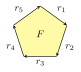
\includegraphics{figures/c12-fig01.svg}\end{center}

Define the map
\begin{align*}
\<\, \>_F\colon A^{\otimes \ov{\del F}}&\to \kk\\
                a_1\otimes \dots\otimes a_k&\mapsto \<a_1, \dots, a_k\>.
\end{align*}
\leref{l:k-pairing} implies that this map does not depend on which edge we
denote by $r_1$ and thus is well-defined.

\begin{remark}
  The reason for choosing $\ov{\del F}$ rather than $\del F$ is that we want
  to think of $F$ as a cobordism from $\ov{\del F}$ to the empty set.
\end{remark}

Since $M$ is a manifold, every unoriented edge appears twice as a boundary
edge of a 2-cell, and every oriented edge appears once as part of $\del F$.
Thus, by taking the tensor product of $\<\, \>_F$ over all 2-cells $F$, we
get a linear map
$$
  \bigotimes_F \< \, \>_F \colon A^E\to \kk.
$$

Let us now put it all together and define a number $Z_A(M,K)\in \kk$ by
\begin{equation}\label{e:fhk-state-sum}
  Z_A(M,K)= \Bigl(\bigotimes_F \< \, \>_F\Bigr)
          \Bigl(\prod_v(w^{-1}_v) \Bigr)e_M\in \kk
\end{equation}
where $e_M$ is defined by \eqref{e:eM} and $w_v$ is defined by \eqref{e:wv}.

%FIXME: picture with dual graphs.

\begin{theorem}\label{t:fhk1}
  Let $M$ be a closed oriented 2-manifold with PLCW decomposition $K$. Let
  $Z_A(M,K)$ be defined by \eqref{e:fhk-state-sum}.
  \begin{enumerate}
    \item So defined $Z_A(M,K)$ does not depend on the choice of an edge $r(v)$
      used to define $w^{-1}_v$.
    \item So defined $Z_A(M,K)$ does not depend on the choice of cell
      decomposition $K$.
  \end{enumerate}
\end{theorem}
\begin{proof}
  Part (1) follows from two observations:
  \begin{itemize}
    \item
      $$
      \sum w^{-1}x_i\otimes x^i=
      \sum x_i\otimes x^i w^{-1}=
      \sum x_i\otimes w^{-1}x^i
      $$
      (the first identity uses the centrality of $e$, the second uses the fact
      that  $w^{-1}$ is central). This shows that replacing a choice of edge
      $r(v)$ by the same edge but with opposite orientation does not change the
      vector $w^{-1}_ve_M$ and thus, does not change $Z_A(M,K)$.
    \item
      If $r_i$, $r_{i+1}$ are two edges of the boundary of some cell $F$ both
      adjacent to vertex $v$, as shown below, then replacing
      $r(v)=r_i$ by $r(v)= r_{i+1}$ does not change the composition
      $\Bigl(\bigotimes_F \< \, \>_F\Bigr)w^{-1}_v$ and thus, does not
      change $Z_A(M,K)$. Indeed, it follows from
      $\<\dots, a_{i}w^{-1}, a_{i+1}, \dots\> =
      \<\dots, a_{i}, w^{-1}a_{i+1}, \dots\>$.

      \begin{center}
      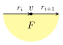
\includegraphics{figures/c12-fig02.svg}
      \end{center}

  \end{itemize}
  By using these two operations, we can replace any oriented edge adjacent
  to $v$ by any other edge. This proves part (1) of the theorem.

  To prove part (2), we need to verify that $Z_A(M,K)$ is invariant under
  elementary moves described in \firef{f:plcw-moves-2}.

  Invariance under subdivision of a 2-cell follows from \eqref{e:k-pairing-2}.

  Invariance under subdivision of a 1-cell follows from
  \begin{center}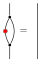
\includegraphics{figures/c12-fig03.svg}\end{center}
  where the red dot stands for the operator of multiplication by $w^{-1}$
  (which comes from the operator $w^{-1}_v$ for the newly added vertex). But
  this is immediate from the definition: indeed, comultiplication is given
  by $\De(a)=\sum a x_i \otimes x^i$, so the composition in the left-hand
  side is $a\mapsto \sum a x_i w^{-1}x^i=a$.
\end{proof}
\begin{remark}
  Note that without the $w^{-1}_v$ factor, this theorem would fail unless
  we assume $\sum x_ix^i=1$.
\end{remark}

Thus, we see that \eqref{e:fhk-state-sum} defines an invariant of closed
2-manifolds. In the next section, we will generalize it to manifolds with
boundary, thus defining an extended TQFT as a lattice theory.

\begin{example}\label{x:lattice-S2}
  Consider the PLCW decomposition of $S^2$ obtained by gluing together
  opposite edges of the bigon shown below.
  \begin{center}
\includegraphics{figures/c12-eqfig01.svg}\end{center}
  This cell decomposition has one 2-cell, one 1-cell, and two vertices.
  The state sum \eqref{e:fhk-state-sum} in this case gives
  $$
    Z_A(S^2)=\sum \eps(w^{-2}x_ix^i)=\eps(w^{-1}).
  $$
\end{example}

\begin{example}\label{x:lattice-T2}
  Consider a PLCW decomposition of the torus $T^2$
  obtained by gluing together opposite sides of the rectangle. This
  decomposition has a single 2-cell, two edges, and one vertex.
  The state sum \eqref{e:fhk-state-sum} in this case gives
  $$
    Z_A(T^2)=\sum \eps(w^{-1}x_ix_jx^ix^j)=\sum (p(x_j),x^j)=  \tr_A (p)
  $$
  where $p\colon A \to A$ is given by $p(a)=\sum w^{-1}x_iax^i$. By
  \eqref{e:center-projector}, the so-defined $p$ is exactly the operator of
  projection onto the center of $A$; thus,
  $$
   Z_A(T^2)= \tr_A (p)=\dim z(A).
  $$
\end{example}

%%%%%%%%%%%%%%%%%%
\section{Lattice theory as an extended TQFT}\label{s:lattice-extended}
So far, we have defined $Z_A(M)$ for a closed 2-manifold $M$. However, we
can easily turn it into a fully extended TQFT.

Namely, we define
$$
Z_A(\bullet^+)=A, \qquad
Z_A(\bullet^-)=A^\op
$$

For an oriented 1-manifold $N$ (possibly with boundary), we choose a cell
decomposition of it (which for 1-dimensional manifolds just means choosing
some points that divide $N$ into intervals) and define
\begin{equation}\label{e:ZAN-def}
  Z_A(N) =\Bigl( \bigotimes_{r\in E} A_r\Bigr) /\sum_v I_v
\end{equation}
where for a vertex $v$, the subspace $I_v$ is generated by the elements
$$
  (\dots \otimes a' x\otimes a'' \otimes \dots)
- (\dots\otimes a'\otimes xa''\otimes \dots ), \qquad x\in A
$$
where $a', a''$ are elements in the copies of $A$ assigned to the two edges meeting at $v$ as in the figure below.

\begin{center}
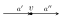
\includegraphics{figures/c12-fig04.svg}
\end{center}

It is trivial to check that the so-defined vector space does not depend on the
choice of cell decomposition (up to a canonical isomorphism); namely,
\begin{equation}\label{e:ZAI-ZAS1}
  \begin{aligned}
    Z_A(I)&=A\otimes_A A\otimes_A \dots \otimes_A A\simeq A\\
    Z_A(S^1)&\simeq A/[A,A].
  \end{aligned}
\end{equation}

If $I$ is an interval, then $Z_A(I)$ is an $A$-bimodule; thus, if we consider
$I$ as a cobordism $\bullet^+\to \bullet^+$, then $Z_A(I)$ is a morphism $A\to
A$ in $\Alg$. We can also consider $I$ as a cobordism
$\bullet^+\sqcup\bullet^-\cob{}\varnothing$, and $Z_A(I)$ as a right module
over $A\otimes A^\op$, or consider $I$ as a cobordism
$\varnothing\cob{}\bullet^+\sqcup\bullet^-$, and $Z_A(I)$ as a left module over
$A\otimes A^\op$.


We can now define $Z_A$ for a 2-cobordism. First, let $M$ be a 2-manifold with
boundary, considered as a cobordism $N\to \varnothing$, where $N=\ov{\del M}$.
Choose a cell decomposition $K$ of $M$; let $E_{\mathrm{bulk}}$ be the set of
oriented edges inside $M$ (thus, every internal unoriented edge of $K_1$
appears twice in $E_{\mathrm{bulk}}$) and $E_{N}$ be the set of oriented edges
on the boundary (each appearing with orientation inherited from $N=\ov{\del
M}$).

Let us modify \eqref{e:fhk-state-sum} and define
\begin{equation}\label{e:fhk-state-sum2}
  Z_A(M,K)= \Bigl(\bigotimes_F \< \, \>_F\Bigr)
  \Bigl(\prod_v(w^{-1}_v) \Bigr)e_M\colon A^{\otimes E_N}\to \kk.
\end{equation}
(note that $e_M\in A^{\otimes E_{\mathrm{bulk}}}$, and $\bigotimes_F \< \, \>_F$ is
a map $A^{\otimes E_{\mathrm{bulk}}\sqcup E_N}\to \kk$). Note that we only take the
product $\prod_v w^{-1}_v$ over \emph{internal} vertices of $K$ and do
not include the vertices on the boundary.

\begin{theorem}\label{t:fhk2}
  \par\noindent
  \begin{enumerate}
    \item The linear map $A^{\otimes E_N}\to \kk$
      defined by \eqref{e:fhk-state-sum2} descends to a
      map $Z_A(N)\to \kk$.
    \item The so-defined operator is independent of the choice of a cell
      decomposition of $M$.
    \item For a closed oriented one-dimensional manifold $N$, let
      $M=N\times I$ considered as a cobordism $N\sqcup \ov{N}\to
       \varnothing$. Then the map
    \begin{equation}\label{e:fhk-pairing}
      Z_A(N\times I)\colon Z_A(N)\otimes Z_A(\ov{N})\to \kk
    \end{equation}
    defined by \eqref{e:fhk-state-sum2}, is a non-degenerate bilinear pairing.
  \end{enumerate}
\end{theorem}
We leave the proof of this theorem to the reader; it is an easy
modification of the proof of \thref{t:fhk1}.

Since the pairing \eqref{e:fhk-pairing} is non-degenerate, it can be used to
identify $Z_A(\ov{N})\simeq (Z_A(N))^*$. In particular, it shows that if $M$ is
a cobordism $N_1\cob{M}N_2$ --- which can also be considered as a cobordism
$N_1\sqcup \ov{N_2}\cob{} \varnothing$ --- then $Z_A(M)\colon Z_A(N_1)\otimes
Z_A(\ov{N_2}) \to \kk$ can also be considered as an operator $Z_A(N_1)\otimes
Z_A(N_2)^*\to\kk$, or equivalently, as an operator $Z_A(N_1)\to Z_A(N_2)$; more
formally, for such a cobordism we define $Z_A(M)\colon Z_A(N_1)\to
Z_A(N_2)$ by
\begin{equation}\label{e:fhk-state-sum3}
  \<Z_A(M)x, y\>= Z_A(M)(x\otimes y), \qquad x \in Z_A(N_1), y \in Z_A(\ov{N_2})
\end{equation}
where $\<\, , \,\>$ is the pairing \eqref{e:fhk-pairing}.

\begin{theorem}\label{t:latticeTQFT}
  Formulas \eqref{e:fhk-state-sum2}, \eqref{e:fhk-state-sum3} define a
  (non-extended) 2-dimensional TQFT.
\end{theorem}

\begin{example}\label{x:lattice-disk}
  Let $D$ be a disk considered as a cobordism $S^1\to\varnothing$. Then
  $Z_A\colon A/[A,A]\to \kk$ is given by the counit of the Frobenius algebra:
  $Z_A(x)=\eps(x)$.
\end{example}
\begin{example}\label{x:lattice-cylinder}
  Let $M=S^1\times I$ be the cylinder considered as a cobordism
  $S^1\sqcup S^1\to \varnothing$. Choosing a decomposition of the cylinder
  obtained by gluing together two sides of the rectangle, we see that in
  this case we have
  $$
    Z_A(M)(a\otimes b)=\sum \eps (ax_ibx^i)
    =\sum \eps(w^{-1} x_jax^jx_i b x^i).
  $$
\end{example}
\begin{exercise}\label{ec:lattice-pants}
  Show that 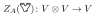
\includegraphics{figures/c12-eqfig02.svg}, where $V=Z_A(S^1)=A/[A,A]$,
  is given by
  $$
    Z_A([a]\otimes[b])=\sum [a x_i b x^i].
  $$
\end{exercise}

Comparing it with \thref{t:centerTQFT}, which gave an explicit description of
the (non-extended) TQFT constructed using Morse decompositions of cobordisms,
we see that these two descriptions match.


Finally, let us define an $Z_A$ as an extended TQFT. We have already defined
$Z$ for 0-dimensional manifolds and 1d cobordisms; thus, to complete the story,
we need to define $Z_A(M)$ for a 2-cobordism, i.e., a 2-manifold with corners
(see \deref{d:2-cobordism}).

\begin{center}
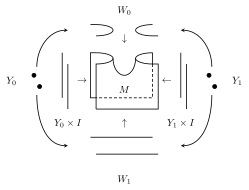
\includegraphics{figures/c12-fig05.svg}
\end{center}


To do that, note that in this case, boundary $\del M$ consists of 3 pieces
(possibly disconnected): $W_0$ (top), $W_1$ (bottom), and ``vertical'' boundary
$Y\times I$, where $Y=Y_0\sqcup Y_1$.

Choosing a cell decomposition $K$ of $M$ such that each corner is a vertex of
that decomposition and using again the formula \eqref{e:fhk-state-sum2}, we can
define
$$
\tilde Z_A(M,K)\colon A^{\otimes E_\ttop}\otimes A^{\otimes E_\bbot}
                \otimes A^{\otimes E_v} \to \kk
$$
where $E_\ttop$, $E_\bbot$, $E_v$ are oriented edges at top, bottom, and
vertical parts of the boundary respectively.

Now, for each vertical edge $e\in E_v$, take vector $1\in A_e$. This
defines a vector $1_v\in A^{\otimes E_v}$. Define
\begin{equation}\label{e:fhk-state-sum3}
  \begin{aligned}
    Z_A(M,K)\colon A^{\otimes E_\ttop}\otimes A^{\otimes E_\bbot}&\to \kk\\
    Z_A(M,K) (a_\ttop\otimes a_\bbot)&=
            \tilde Z_A(a_\ttop\otimes a_\bbot \otimes 1_v).
  \end{aligned}
\end{equation}

% we get the following result.
%\begin{theorem}\label{t:latticeTQFT2}
% For a separable symmetric Frobenius algebra $A$,
% the \textup{(}non-extended\textup{)} TQFT defined by state-sum formulas
% \eqref{e:fhk-state-sum2}, \eqref{e:fhk-state-sum3} coincides with the
% \textup{(}non-extended\textup{)} TQFT defined in \chref{c:2d-extended}.
%\end{theorem}


%%%%%%%%%%%%%%%%%%%%%%%%%%%%%%%%%%%%%%%
\section{Finite group gauge theory as lattice theory}\label{s:lattice-gauge}
Let us consider a special example, which we have already discussed using a
different approach in \exref{x:DW-extended}, namely when the algebra $A=\kk[G]$
is the group algebra of a finite group $G$ and Frobenius structure is given by
$$
  \eps(g)=\de_{g,1} = \frac{1}{|G|}\tr_R(g), \qquad g\in G,
$$
where $R$ is the regular representation.

In this case the element $e=\sum x_i\otimes x^i\in A\otimes A$ is given by
$$
  e=\sum_{g\in G}g\otimes g^{-1}
$$
so that $w=|G|$.

In this case, the map $\<\, , \,\>$ is given by
$$
\<g_1, \dots, g_k\>=\begin{cases}
                     1, & g_1\dots g_k=1\\
                     0, & \text{otherwise}
                   \end{cases}
$$
Thus, one easily sees that for a closed 2-manifold $M$
the state-sum \eqref{e:fhk-state-sum} becomes
$$
Z_A(M,K)=\frac{1}{|G|^V} \sum_{c} 1
$$
where $V$ is the number of vertices of $K$ and  the sum is over all
``colorings'' of edges, i.e., ways of assigning a group element $g_r$ to each
oriented edge $r$ so that for two opposite orientations of the same edge,
$g_{r'}=g_{r''}^{-1}$ and such that the product of colors over the boundary of
any 2-cell is equal to 1.

One easily sees that it is a discrete version of a connection in $G$-bundles:
without the factor $\frac{1}{|G|^V}$, this counts $G$-bundles on $M$ together
with trivializations at every vertex. Thus, dividing by $|G|^V$ exactly gives
the number of $G$-bundles on $M$ counted as in \chref{c:DW}; in other words,
this recovers the Dijkgraaf--Witten TQFT.


%!TEX root = TQFTbook.tex
%%%%%%%%%%%%%%
\chapter{2d TQFT with defects}\label{c:2d-defects}


So far we only considered TQFTs defined on homogeneous spacetimes, where the
local structure of the theory is the same at every point of the spacetime.
However, one can also consider theories where different parts of the spacetime
carry different TQFTs. The codimension-one locus separating the homogeneous
parts should describe interface between different TQFTs; moreover, one can
continue, introducing a codimension 2 stratum separating different codimension
1 interfaces. In physics, all these positive codimension strata are thought of
as a \emph{defects}\index{defect} in the structure of spacetime, and the
corresponding formalism is referred to as \emph{TQFT with
defects}\index{TQFT!with defects}. As we will show later, this approach
is very closely related to fully extended TQFT (see section FIXME below).

This idea has a long history in physics. Our exposition follows  \cite{dkr},
which gives a detailed description of 2D TQFT with defects. See also review
articles \cite{carqueville} and \cite{cdr}. Very closely related formalism in
the context of extended TQFTs is also described in \cite[Section 4.3]{lurie}
under the name \emph{TQFT for manifolds with singularity}. For simplicity, we
restrict ourselves to the 2-dimensional case.

% Wrapping the Tikz commands in an environment so that they don't interefere with other chapters.
\begin{defectfiguresetup}
%%%%%%%%%%%%%%%%%%%%%%%%%%%%%%%%%%%%%%%%%%%%%%%%%%%%%%%%%%%%%
\section{Data for TQFT with defects}\label{s:defect-data}
Recall that we have defined a two-dimensional extended TQFT as a symmetric
monoidal functor $Z\colon \Bord_2\to \calC$, where $\calC$ is a (weak)
2-category; such a theory is uniquely determined by a fully dualizable object
$A\in \calC$. In particular, it assigns an invariant $Z_A(M)\in
\End_\calC(\one)$ to every closed manifold $M$; equivalently, we can say that
it assigns an invariant $Z(M,A)$ to every pair $(M, A)$, where $M$ is a closed
2-manifold and $A\in \calC$ is a fully dualizable object. We can think of pair
$(M,A)$ as a \emph{colored manifold}, i.e. a manifold together with some extra
data (coloring), which in this case consists of choosing an object $A$.

For theory with defects, we need to modify this definition in two ways. First,
instead of usual bordisms, we need to define bordisms with defects,  as
outlined in introduction to this chapter. Second, we neeed to define the notion
of coloring, i.e. assignign appropriate alegbraic data to different strata.
Aftre that, we will be able to define an extended TQFY with defects as a
symmetric monoidal functor
$$
Z^{\mathrm{defect}}\colon \Bord_2(\calC)\to \calC.
$$
where $\Bord_2(\calC)$ is the 2-category of $\calC$-colored stratified oriented
2-bordisms.


We begin by defining closed manifolds
with defects, or \emph{stratified manifolds}.

\begin{definition}\label{d:stratified_manifold}
  A \emph{stratified 2-manifold}\index{stratified manifold} is an
  oriented closed 2-manifold $M$ together with  decomposition
  $$
    M=M_2\sqcup M_1\sqcup M_0
  $$
  where each $M_i$ is a (not necessarily compact) locally closed submanifold
  of dimension $i$ in $M$ such that:
  \begin{itemize}
    \item $M_2$ is open and dense in $M$
    \item Every point $x\in M_1$ has a neighborhood which looks like shown in
    FIXME
    \item Every point $x\in M_0$ has a neighborhood which looks like shown in
    FIXME
  \end{itemize}
\end{definition}
We will refer to $M_1$ and $M_0$ as strata of dimension 1 (respectively, 0);
physicists would also call them defect lines and point defects respectively.

An example of a stratified manifold is shown in
\firef{f:stratified_pretzel} below.

In a similar way one can define the notion of a stratifed manifold with boundary
or a stratified cobordism; in this case, we need to require additionally that
the stratification meets the boundary transversally (in particular, it means
that the codimesion 2 strata should not be on the boundary).


	\begin{figure}[ht]
	\centering
	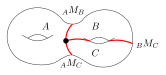
\includegraphics{figures/c13-fig01.svg}
	\caption{A stratified manifold decorated with algebras $A$, $B$ and $C$ on
	different regions. Defects are shown in red, and are labelled by bimodules.
	Defects require a choice of orientation, which is suppressed here for
	brevity.}
	\label{f:stratified_pretzel}
\end{figure}

Next, we should define the notion of coloring. We do it first in a very special
case, namely when the manifodl $M$ is closed and the target category $\calC$ is
the category of associative algebras. As was previously discussed, fully
dualizable objects in this category are finite-dimensional semisimple algebras,
and for construction of an extended TQFT one needs a semisimple algebra with
extra data, namely with the structure of a symmetric Frobenius algebra.

Before the continuing, let us note that we assume that $M$ is oriented;
however, we do not assume any choice of orientation on defect lines (that is,
connected components of $M_1$). Note that since $M$ is oriented, choosing an
orientation of $M_1$ is equivalent to chooisng orientation of the normal bundle
to $M_1$

\begin{definition}\label{d:defect-coloring}
  Let $M$ be a closed oriented stratified 2-manifold, and let $\calC=\Alg$ be
  the 2-category of alegbras and bimodules as defined in \exref{x:alg}. A
  $\calC$-coloring of $M$ is the following data:
  \begin{itemize}
    \item A choice of a semisimple symmetric Frobeinus algebra $C(U)$ for each
    connected component $U$ of the open strata $M_2$

    \item A choice of a 1-morphism (that is, a bimodule) $M=C(Y)$ for every
    connected component $Y$ of $M$ together with orientation of $Y$. More
    precisely, if $Y$ separates regions colored by algebras $A$ and $B$ as
    shown below, then it should be colored by a finite-dimensional  $B$-$A$
    bimodule $M$.

    Moreover, we require that the bimodules corresponding to opposite choice of
    orientation are duals (in the sense of vectro spaces) of each other. FIXME:
    better wording.

    \item
        For each vertex $u \in M_0$, we need a multilinear map $\ph_u$ from
        cyclic tensor product of incident bimodules to the field $\kk$.

    		\begin{figure}[ht]
    			\centering
    			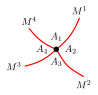
\includegraphics{figures/c13-fig02.svg}
    			\label{f:junction}
    		\end{figure}

    		For example, if the junction looks like as given above, then it is
    		assigned a map:

    		\begin{equation}\label{e:junction-data}
    			\varphi: \circlearrowleft_{A_1} ( M^1 \otimes_{A_2}  M^2
    			\otimes_{A_3} M^3 \otimes_{A_4} M^4  ) \rightarrow  \kk
    		\end{equation}

    		 Here, $\circlearrowleft_{A} M$ is the cokernel of the map $A \otimes M
    		 \rightarrow M, a \otimes m \mapsto am - ma$. This property of
    		 $\varphi$ ensures that the junction has no preferred starting edge.
    		 See \cite[Section 2.3]{carqueville} for another motivation behind
    		 this data.
  \end{itemize}
  We will refer to a pair $(M, C)$, where $M$ is an oriented manifold and $C$
  is $\calC$-coloirng of $M$ as a \emph{$\calC$-colored
  manifold}.\index{stratified manifold!$\calC$-colored}
\end{definition}

%%%%%%%%%%%%%%%%%%%%%%%%%%%%%%%%%%%%%%%%%%%%%%%%%%%%%
\section{State sum construction of TQFT with defects}\label{s:defect-statesum}

In this section we sketch the construction of the TQFT with defects, i.e., a
functor $Z^{\mathrm{defect}}\colon \Bord_2(\calC)\to \calC$, using state sum
approach.  As before, we only consider the target category $\calC=\Alg$. For
simplicity, in this section we only explain how one defines $Z(M,C)$ for a
colored stratified closed 2-manifold $M$; generalization of this to cobordisms
will be explained in the next section. Our exposition follows \cite{dkr} with
minor changes, though their notation differs from ours (in particular, they use
$T^{\mathrm{cw}}$ for what we denote by $Z\equiv Z^{\mathrm{defect}}$).

The state sum construction below is a generalization of construction in
\chref{c:2d-lattice}. Thus, given $\calC$-colored stratified closed 2-manifold
$M$, we begin by choosing a PLCW decomposition $K$ of it; we require that this
PLCW decomposition is transversal to the stratification.


As in \seref{s:state-sum}, we denote by $K_2$ the set of 2-cells of $K$, by
$K_1$ the set of 1-cells (edges), and by  $K_0$, the set of vertices. Further,
we assume that every edge $r\in K_1$ has at most one intersection with the
defect lines, i.e. stratum $M_1$, and each 2-cell $F$ of the decopmosition
contains at most one point from $M_0$. An examples of such PLCW decomposition
of a stratified manifold is shown in \firef{f:vectors-on-edges}.



As in \seref{s:state-sum}, we will denote by $E$ the set of \emph{oriented}
edges of $K$, i.e., pairs consisting of an edge $r\in K_1$ and an orientation
of $r$. Thus, every (unoriented) edge $r\in K_1$ gives rise to two oriented
edges $r', r''\in E$. To every oriented edge $r\in E$, we assign a vector space
$Q_r$ s follows:
\begin{equation}\label{e:q-definition}
	Q_{r} =
	\begin{cases}
		A, & \text{if $r$ does not cross a defect line and lies within component of
		$M_2$ colored by algebra $A$ },\\
		X, & \text{if $r$ crosses defect line which is colored by bimodule $X$,
    with orientation as shown below FIXME}
	\end{cases}
	\end{equation}

We define an intermediate vector space $Q(M)$ by tensoring the contribution of
\begin{equation}\label{e:Qr}
	Q(M) = \bigotimes_{r\in E} Q_r.
\end{equation}
Note that in the special case of a manifold without stratification, this
coincides with vector space $A^E$ as defined in \eqref{e:AE}.

Note that each (unoriented) edge $r\in K_1$ gives two factors in $Q(M)$: either
two copies of $A$ (if $r$ does not intersect defect lines) or $X\otimes X^*$,
where $X, X^*$ are the colors of of the defect line crossing $r$ (one
orientation gives $X$, the other, $X^*$).


FIXME

Consider  \firef{f:vectors-on-edges} for example. Edge $e_2$, irrespective of
its orientation, lies entirely in algebra $b$, so it is labelled $A_b$. Edge
$e_1$, within polygon $p_2$, has defect $x$ crossing it such that the defect is
entering $p_2$.  So the triplet $(p_2,e_1,+)$ is labelled $X_x$. The same edge,
within polygon $p_1$, has defect $x$ going out of the polygon. So it is
labelled $X_x^*$ for the triplet $(p_1,e_1,+)$.  We only consider those
triplets where the orientation matches with that of the polygon. We would have
to consider both orientations of an edge ( i.e. for example $(p_1,e_1,+)$ as
well as $(p_1,e_1,-)$ ) only when the polygon closes on itself through that
edge. See \cite[Section 3.5]{dkr} for an example.

\begin{figure}[ht]
	\centering
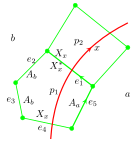
\includegraphics{figures/c13-fig03.svg}
			\caption{Example of vector spaces assigned to the edges of 2-cell $p_1$. Regions to the left and right of defect $x$ are labelled by algebras $b$ and $a$ respectively.}
			\label{f:vectors-on-edges}
\end{figure}

Next, for every (unoriented) edge $r$ we define a vector
$$
e_r = \sum x_i \otimes x^i\in Q_{r'}\otimes Q_{r''}
$$
where $r'$, $r''$ are two orientations of $r$. Namely,
\begin{itemize}
  \item If $r$ doesn't intersect defect lines so that $Q_{r'}\otimes
  Q_{r''}=A\otimes A$, then $x_i, x^i$ are dual bases in $A$ with respect to
  Frobenius pairing (compare with \eqref{e:er}).
  \item If $r$ intersects a defect line labelled by bimodule $X$ or $X^*$
  (depending on orientation), then $x_i, x^i$ are dual bases in $X$, $X^*$.
\end{itemize}

Taking product over all unoriented edges $r\in K_1$, we get a vector
$$
e_M=\bigotimes_{r\in K_1} e_r\in Q(M)
$$
(compare with \eqref{e:eM}).


FIXME: algebraic data defined by vertices??


Finally, for a 2-cell $F$ of $K$, we define the space
$$
Q_F=\bigotimes_{r\in \ov{\del F}}Q_r
$$
where the tensor product is taken in clockwise order, and
a map
$$
\eps_F \colon Q_F\to \kk
$$
as follows.

\begin{enumerate}
	\item[I.]
    If the 2-cell contains a single vertex $v\in M_0$, and for each edge $r$ of
    $F$ there is a unique defect line passing through that edge, then we
    define
    \begin{equation}
      \eps_F=\ph_v\colon X_1\otimes_{A}\dots \otimes X_k\to \kk
		\end{equation}
    (the product is taken in clockwise order).

    If $F$ contains a vertex, but certain edges don't intersect any defect
    lines, we multiply the colors of these edges and the color of the adjacent
    bimodule elements, as illustrated by the figure below.

FIXME

  \item[II.]
    If the cell $F$ has no vertex and contains a unique defect line, colored by
    $X$ and crossing two edges of $F$, then we add on this line a single vertex
    $v$ colored by $\ph_v=\ev_X\colon X^*\otimes X\to \kk$, and then use the
    previous construction.

	\item[III.] If no defect line passes through $F$, and $F$ lies in region
    labelled by algebra $A$, then
    $$
    \eps_F(a_1 \otimes \cdots\otimes  a_k) = \eps_{A}(a_1 \cdots a_k)
    $$
    (compare with \eqref{e:epsF}).
\end{enumerate}

Note that case  III can be considered as special case of I, if we allow
ourselves adding ``trivial'' defect lines, colored by ${}_AA_A$,  in any region
colored by algebra $A$.

As before, taking the tensor product over all 2-cells  $F\in K_2$ and observing
that $\bigotimes_F Q_F=Q(M)$ (which follows from the fact that every unoriented
edge of $K$ appears exactly twice as a boundary of some 2-cell, with opposite
orientations), we can define the map
$$
\eps_M=\bigotimes_{F\in K_2} \eps_F \colon Q(M)\to \kk.
$$

We now define the invariant of a $\calC$-colored stratified manifold $M$
with a given cell decomposition $K$ by
\begin{equation}\label{e:defect-state-sum}
  Z(M,C,K)=\eps_M (e_M)
\end{equation}
(compare with \eqref{e:fhk-state-sum}). FIXME: $w^{-1}$??


The functor $Z$ for a bordism $M:U\rightarrow V$ is defined as:
\begin{equation}
	Z(M) : Z(U) \xto{id_{Z(U)} \otimes P(M)} Z(U) \otimes Q(M) \otimes Z(V) \xto{E(M) \otimes id_{Z(V)}} Z(V)
\end{equation}

We explain $Z(U), Z(V), P(M), E(M)$ next.


Let's define the functor on a (decorated) circle $O$ first. For a more general object $U=O_1 \sqcup O_2 \sqcup \cdots \sqcup O_n$, we then have $Z(U)=Z(O_1)\otimes Z(O_2) \otimes \cdots \otimes Z(O_n)$. As a 1-dimensional space, a circle doesn't need 2-cells for its decomposition.  \cite[Section 2.3]{dkr} provides a construction using collars to assign a vector space to decorated circles with just this data. But we will reuse the following equivalent boundary convention. For a circle $O$ lying on $\partial_{in} M$, we assign the same vector space to each edge as was defined in \eqref{e:q-definition}. For a circle lying on $\partial_{out} M$, we still use the \eqref{e:q-definition}, but dualize the $X$ type vector spaces.

The map $P(M): \kk \rightarrow Q(M) \otimes Z(V)$ is defined as:
\begin{equation}
	P(M) = \bigotimes_{e \in C_1(M), e \notin \partial_{\mathrm{in}} M} P_e
\end{equation}

For an edge $e$ intersecting a defect $x$, the propagator map $P_e: \kk \rightarrow Q_{p(e)_1,e,\mathrm{or}_1} \otimes Q_{p(e)_2,e,\mathrm{or}_2}$ comes from a basis $\sum_{i} u_i \otimes u_i^* \in X_x \otimes X_x^*$. For an edge that does not intersect any defect, and is contained in Frobenius algebra $a$, the map $P_e$ comes from the coevaluation map $\beta_{A_a}$ of the algebra $a$.

We then define the evaluation map $E_p: \bigotimes_{(e,\mathrm{or}) \in \partial p} Q_{p,e,\mathrm{or}} \rightarrow \kk $ for each polygon $p$ as:
\begin{enumerate}
	\item[I.] If no defect line passes through $p$, and $p$ lies in region labelled by algebra $a$, then $E_p(q_1 \otimes \cdots q_m) = \eps_{A_a}(q_1 \cdots q_m)$. This is the same map which was used for TQFT without defects ( see  \eqref{e:k-pairing} ).
	\item[II.] Let's say a defect line $x$  passes through two edges such that $q_1 \in X_x^*$ ( outgoing ) and $q_i \in X_x$ ( incoming) , then $E_p(q_1 \otimes \cdots q_m) = q_1 ( (q_2 \cdots q_{i-1}).q_i.(q_{i+1}\cdots q_m))$. Recall that $q_i$ is a bimodule on which appropriate algebra elements can act from right or left sides, and $q_1$ lives in the dual bimodule space.
	\item[III.] If the 2-cell contains a junction such that one domain wall passes through each edge of the 2-cell, we use the map $\varphi_p$, defined in \eqref{e:junction-data}, to assign an element of $\kk$ as:
	\begin{equation}
		E_p(q_1 \otimes \cdots \otimes q_m)=\varphi_p \circ \pi_\otimes(q_1 \otimes \cdots \otimes q_m)
	\end{equation}
	$\pi_\otimes: X_{x_1}^{\epsilon_1} \otimes_{A_2} \cdots \otimes_{A_m}  X_{x_m}^{\epsilon_m} \rightarrow \circlearrowleft_{A_1} (X_{x_1}^{\epsilon_1} \otimes_{A_2} \cdots \otimes_{A_m}  X_{x_m}^{\epsilon_m}) $ is a projection to the cylic tensor product on which $\varphi_p$ acts. If $p$ contains a junction, but certain edges don't intersect any domain wall, we can still use this definition of $E_p$ by multiplying its algebra elements with an adjacent bimodule.
\end{enumerate}

%This image is floating into the next section. So I decided to insert it directly instead of inserting as an image
\begin{center}
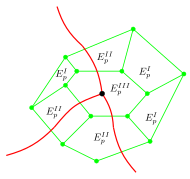
\includegraphics{figures/c13-fig04.svg}
\end{center}

For example, for the defect network shown above, we indicate by subscripts as to which definition of $E_p$ will be used in different polygons. Altogether, the evaluation map $E(M)$ is then defined as:

\begin{equation}
	E(M) = \bigotimes_{p \in C_2(M)} E_p
\end{equation}

This completes the definition of the functor $Z$. In the special case where the bordism has no boundary, we have $\partial_{\mathrm{in}} = \partial_{\mathrm{out}} = \emptyset$. Then $Z$ is just a map from $\kk$ to $\kk$, which is just an element of $\kk$.

\section{Independence of cell decomposition}\label{s:decomposition-independence}
We had to use a cell decomposition in the last section to define the functor $Z$. Since cell decomposition is not a part of the actual defect TQFT data, we need to prove that the state sum construction is independent of our choice of cell decomposition. The key part of the proof is the following lemma.

\begin{lemma}\label{l:invariance-under-local-moves}
	For two colored bordisms $M$ and $M'$, $Z(M) = Z(M')$ if the cell decompositions of $M$ and $M'$ are related by one of the following classes:
	\begin{enumerate}
		\item Addition of an edge with a vertex to a 2-gon

		\newcommand{\twogonA}{%
			\vcenter{\hbox{%
					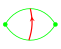
\includegraphics{figures/c13-fig05.svg}%
			}}%
		}

		\newcommand{\twogonB}{%
			\vcenter{\hbox{%
					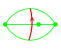
\includegraphics{figures/c13-fig06.svg}%
			}}%
		}

		\newcommand{\twogonC}{%
			\vcenter{\hbox{%
					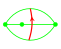
\includegraphics{figures/c13-fig07.svg}%
			}}%
		}

		\begin{align*}
			\twogonA \leftrightarrow \twogonB \leftrightarrow \twogonC
		\end{align*}

		\item Addition of an edge inside an n-gon

		\newcommand{\pentagonA}{%
			\vcenter{\hbox{%
					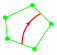
\includegraphics{figures/c13-fig08.svg}%
			}}%
		}

		\newcommand{\pentagonB}{%
			\vcenter{\hbox{%
					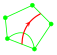
\includegraphics{figures/c13-fig09.svg}%
			}}%
		}

		\newcommand{\pentagonC}{%
			\vcenter{\hbox{%
					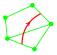
\includegraphics{figures/c13-fig10.svg}%
			}}%
		}

		\newcommand{\pentagonD}{%
			\vcenter{\hbox{%
					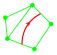
\includegraphics{figures/c13-fig11.svg}%
			}}%
		}


		\newcommand{\pentagonE}{%
			\vcenter{\hbox{%
					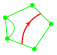
\includegraphics{figures/c13-fig12.svg}%
			}}%
		}

		\begin{align*}
			 \pentagonA \leftrightarrow \pentagonB \leftrightarrow \pentagonC \leftrightarrow \pentagonD \leftrightarrow \pentagonE
		\end{align*}

		Apart from the pentagons shown above, the other diagrams included in this local move are all the n-gons with $n \ge 3$. The domain wall can run between any two edges.
	\end{enumerate}
\end{lemma}

Note that the defect can also be $A$ itself, which is the same as having no defect at all in the diagrams shown above. We sketch here proofs for two of these moves. Let's first consider a move that inserts an edge and a vertex in a 2-gon, as given in \firef{f:example1-local-modification}.

\begin{figure}[ht]
	\centering

	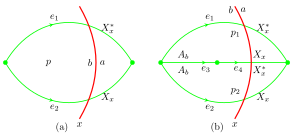
\includegraphics{figures/c13-fig13.svg}

	\caption{Example(I) of a local modification of cell decomposition used in \leref{l:invariance-under-local-moves}}
	\label{f:example1-local-modification}
\end{figure}


The contribution to projector $P$ coming from the new edges $e_3$ and $e_4$ is:
\begin{align*}
	P_{e_3} \otimes P_{e_4}: \kk &\rightarrow (A_b \otimes A_b) \otimes (X_x \otimes X_x^*)\\
												 1 &\mapsto  \sum_i (b_i' \otimes b_i) \otimes \sum_j (u_j \otimes u_j^*)\\
\end{align*}

The total contribution of cells $p_1$ and $p_2$ from the right picture is
\begin{align*}
	& \sum_{i,j} \varphi(b_i'.u_j)\ u_j^{*}(b_i.x)\\
	& =\sum_{i,j} \varphi(b_i'.u_j  (u_j^{*}(b_i.x) ))\\
	& =\sum_{i} \varphi\left(b_i'.\sum_{j}u_j  (u_j^{*}(b_i.x)) \right)\\
	& =\sum_{i} \varphi(b_i'.b_i.x )\\
	& =\varphi(x)
\end{align*}
In the intermediate step, the $\sum_j u_j $ basis has been used to express the bimodule $b_i.x$ as $b_i.x= \sum_j u_j u_j^*(b_i.x)$. The original contribution of cell $p$, shown in the left part of the figure, is also $\varphi(x)$. Similarly we can show that the other local move that divides the 2-gon also leaves the functor $Z$ invariant.


Now, let's consider another example of a local move, given in \firef{f:example2-local-modification}.

\begin{figure}[ht]
	\centering

	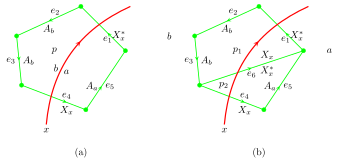
\includegraphics{figures/c13-fig14.svg}

	\caption{Example(II) of a local modification of cell decomposition used in \leref{l:invariance-under-local-moves}}
	\label{f:example2-local-modification}
\end{figure}


The contribution to projector $P$ coming from the new edge $e_6$ is:
\begin{align*}
	P_{e_6}: \kk &\rightarrow X_x \otimes X_x^*\\
	1 &\mapsto  \sum_j u_j \otimes u_j^*\\
\end{align*}

The total contribution of cells $p_1$ and $p_2$ from the right picture is
\begin{align*}
	& \sum_{j} \varphi(b_1.b_2.u_j)\ u_j^{*}(x.a)\\
	& =\sum_{j} \varphi(b_1.b_2.u_j u_j^{*}(x.a) )\\
	& =\varphi(b_1.b_2.x.a)
\end{align*}
This contribution is the same as that of the original pentagon shown in the left part of the figure. The proof for the invariance of functor $Z$ under the remaining local moves can be constructed similarly.


\section{TQFT as special case of defect TQFT}\label{s:tqft-as-dtqft}
A TQFT ( without defect ), with or without boundary, can be thought of as a special case of defect TQFT on a closed manifold. A TQFT without a boundary can be simply obtained by choosing a coloring which contains no defects.

\begin{equation}
	Z^{\mathrm{without\ defect}}_{A} (M) = Z^{\mathrm{defect}} (M; \mathrm{Coloring}={\{A\} ,M_1= \emptyset,M_0=\emptyset})
\end{equation}

We can also get a TQFT, described by separable symmetric Frobenius algebra $A$, on manifold $M$ with a boundary $\partial M$, by choosing appropriate coloring in a defect TQFT. This time, the coloring consists of a defect line $X_{\partial M}$ that runs along the boundary of $M$. This defect TQFT is defined on a closed manifold $\widetilde{M}$ that is an extension of $M$. The region of $\widetilde{M}$ lying outside $M$ is colored by the algebra $\kk$. The region $M$ is colored by algebra $A$. The defect $X_{\partial M}$ is thus an A-module, and in physics language, it separates the ``non-trivial phase'' $A$ from the ``trivial'' phase. For example, the following figure shows a defect TQFT equivalent to a TQFT with a boundary.


\newcommand{\picone}{%
	\vcenter{\hbox{%
			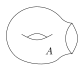
\includegraphics{figures/c13-fig15.svg}%
	}}%
}

\newcommand{\pictwo}{%
	\vcenter{\hbox{%
			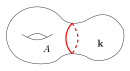
\includegraphics{figures/c13-fig16.svg}%
	}}%
}

\begin{equation}
\picone=U\left(\pictwo\right),
\end{equation}
where $U$ is a forgetful functor that erases the phase labelled by $\kk$, and removes all defect lines. See \cite{carqueville} for detailed construction of a TQFT ( with or without boundary ) from a defect TQFT.

\end{defectfiguresetup}
\clearpage

\part{Cobordism hypothesis}\label{p:cobordism-hypothesis}
%!TEX root = TQFTbook.tex
%%%%%%%%%%%%%%%%%%%%%%%%%%%%%%
In this part, we start discussion of extended TQFTs in
any dimension, formulating the celebrated cobordims hypothesis.

FIXME
\include{c14-higher-cat-src-gerby}
\include{c15-cobordism-hyp-src-gerby}

\part{Tensor categories and Turaev--Viro theory}\label{p:tensor-categories}
%!TEX root = TQFTnotes.tex
%%%%%%%%%%%%%%%%%%%%%%%%%%%%%%
\chapter{3-category of tensor categories}\label{c:3cat-tens}
%References: \cite{dsps-balanced}, \cite{dsps-dualizable},
% \cite{etingof-fusion}.

In the previous chapters, we have given two constructions of an extended
2-dimensional TQFT with values in the 2-category $\Alg$ of algebras and
bimodules: one construction was based on the work of Schommer-Pries, describing
the 2-category $\Bordor_2$ by generators and relations, and the other was based
on triangulations (or more general PL cell decompositions) of a 2-manifold. In
both cases, such a theory is determined by $A=Z(\bullet)$ which must be a
separable symmetric Frobenius algebra. This is a special case of the general
cobordism hypothesis, according to which extended framed $n$-dimensional TQFTs
with values in $\calC$ are described by fully dualizable objects in $\calC$, and
oriented extended TQFTs are described by $\SO(n)$ homotopy fixed points in
$\calC^{\fd}$. In particular, for $n=2$, $\calC=\Alg$, fully dualizable objects
are separable algebras, and $\SO(2)$ homotopy fixed points are
separable symmetric Frobenius algebras.

In this chapter, we start exploring the 3d analog of these constructions. As we
will show, in this case one possible replacement for the 2-category $\Alg$ is
the 3-category $\Tens$ of finite tensor categories, and the fully dualizable
objects in it are exactly semisimple tensor categories, i.e., fusion categories;
$\SO(3)$ homotopy fixed points are (conjecturally) spherical fusion categories.
The corresponding 3-dimensional oriented extended TQFT is known as Turaev--Viro
theory.

In this chapter, we will define and study the 3-category $\Tens$, following
the works \cite{dsps-balanced}, \cite{dsps-dualizable}; the construction of
Turaev--Viro theory will be given in a later chapter.

To simplify the exposition, throughout this chapter we assume that $\kk$ is an
algebraically closed field of characteristic zero. As usual, we will skip most
proofs, referring the reader to original papers.

\section{Review of 2-category $\Alg$}\label{s:alg-review}
For comparison, we recall the main steps in the construction of the 2-category $\Alg$:
\begin{itemize}
  \item We start with the category $\vect$ of $\kk$-vector spaces and define
    the tensor product functor $\otimes\colon\vect\times\vect \to \vect$
  \item Next, we define an algebra $A$ as an object $A\in\vect$ together with
    a morphism $m\colon A\otimes A\to A$ and an element $1\in A$ satisfying
    associativity and unit axioms. We also define the notion of morphisms between
    algebras.
  \item We define the notion of left and right $A$-module and $A$-$B$-bimodules,
  together with module homomorphisms.
  \item Finally, we define the notion of tensor product over an algebra: given right
  $A$-module $M$ and left $A$-module $N$, we define $M\otimes_A N$
\end{itemize}

Let us now proceed to defining categorical analogs of all of the above.

%%%%%%%%%%%%%%%%%%%%%%%%%%%%%%
\section{Finite $\kk$-linear categories}\label{s:finite-categories}
Our first step is defining a 2-category which will replace the category $\vect$.
For that, recall that we have defined the notion of a locally finite
$\kk$-linear abelian category as a $\kk$-linear abelian category where all
objects have finite length and all $\Hom$ spaces are finite-dimensional, see
\seref{s:deligne-product}. Such categories form a 2-category $\Linlf$; this
2-category should be considered a natural categorical analog of the category of
vector spaces.

Let us now consider a more restrictive set of requirements.

\begin{definition}\label{d:finite-linear}
  A $\kk$-linear category $\calA$ is called \emph{finite}
  \index{category!finite} if it satisfies the
  following properties:
  \begin{enumerate}
    \item For any $A,B\in \calA$, the vector space $\Hom_\calA(A,B)$ is
      finite-dimensional.

    \item Any object $A\in \calA$ has finite length.
    \item $\calA$ has enough projectives: any $A\in \calA$ is a quotient of
     a projective object $P\in \calA$.
    \item There are only finitely many isomorphism classes of simple objects.
  \end{enumerate}
\end{definition}
Note that we do not assume that $\calA$ is semisimple.

\begin{example}\label{x:finite-cat-alg}
  Let $A$ be a finite-dimensional algebra over $\kk$. Then the category $A\mod$
  of finite-dimensional $A$-modules is a finite $\kk$-linear category. Moreover,
  it is easy to show that conversely, every finite $\kk$-linear category is
  equivalent to the category $A\mod$ for some finite-dimensional algebra $A$
  (see \cite[Section~1.8]{etingof-fusion}).
\end{example}


Unless stated otherwise, all functors between $\kk$-linear categories will
be assumed to be additive, $\kk$-linear, and right exact.


\begin{definition}\label{d:linf}
  We denote by $\Linf$ the 2-category of finite $\kk$-linear abelian
  categories together with additive and $\kk$-linear right exact
  functors between them and functorial morphisms.
\end{definition}
The so-defined 2-category $\Linf$ is the categorical analog of the category of
finite-dimensional vector spaces.



\begin{remark}
  One might notice that we are not quite consistent: in the $n=2$ case, we started
  with category of all vector spaces, not necessarily finite-dimensional ones,
  so our 2-category $\Alg$ also included infinite-dimensional algebras ---
  which, however, were irrelevant for constructing TQFTs: any fully dualizable
  (i.e., separable) algebra is automatically finite-dimensional. In the $n=3$ case,
  we start with finite linear categories from the beginning.

  The reason is mostly technical; many of the constructions below work for any
  locally finite category (i.e., a category only satisfying the first 2
  conditions of \deref{d:finite-linear}). I expect that one can in fact define a
  version of the (not yet constructed) 3-category $\Tens$ starting with
  locally finite linear categories rather than finite; however, it does create
  some technical difficulties, and since we expect that the only categories we
  will need for extended 3d TQFTs will be finite anyway, we can save some
  trouble and only work with finite linear categories from the beginning.
  \end{remark}

%%%%%%%%%%%%%%%%%%%%%%%%%%%%
\section{Finite tensor categories}\label{s:tensor-categories}
Our next step is defining a categorical analog of the notion of associative
algebra. The obvious candidate is the notion of a monoidal category as
discussed in \chref{c:categories}. However, in order to make some future
constructions possible, we will add some additional conditions.

\begin{definition}\label{d:finite-tensor}
  A \emph{finite tensor category}\index{finite tensor category} is a finite $\kk$-linear category $\calC$
  together with a structure of a monoidal category such that
  \begin{enumerate}
    \item The tensor product functor $\otimes\colon
     \calC\times \calC\to \calC$ is $\kk$-bilinear.
    \item $\Hom(\one, \one)=\kk$.
    \item $\calC$ is rigid: every $X\in \calC$ has left and right dual (see
      \deref{d:rigid}).
  \end{enumerate}
\end{definition}
(Note that we do not give a definition of (not necessarily finite) tensor
category since the only tensor categories we will need are the finite ones.)

Condition (1) is a natural compatibility between the monoidal structure and
structure of $\kk$-linear category; condition (2) is a harmless condition which
is there just for convenience --- almost everything below can be repeated,
possibly with minor changes, without that assumption (in fact,
\cite{dsps-balanced} do not include this condition). But the rigidity condition
(3) is absolutely crucial: without it, most of the theory below would not work.


\begin{lemma}\label{l:tensor-biexact}
  Let $\calC$ be a finite tensor category. Then
  \begin{enumerate}
    \item Functor $\otimes \colon \calC\times \calC\to \calC$ is bi-exact.
    \item Object $\one\in \calC$ is simple.
  \end{enumerate}
\end{lemma}
A proof of this lemma can be found in \cite[Proposition
4.2.1, Theorem 4.3.8]{etingof-fusion}.

As an immediate corollary, we see that tensor product can be considered as a
functor $\calC\boxtimes \calC\to \calC$, where $\boxtimes$ is Deligne's product
of $\kk$-linear categories, see \seref{s:deligne-product} (in the same way as
for algebras, multiplication can be considered as either a bilinear map $A\times
A\to A$ or as a linear map $A\otimes A\to A$).

\begin{lemma}\label{l:tensor-boxtimes}
  Let $\calC$, $\calD$ be finite tensor categories. Then category
  $\calC\boxtimes \calD$ has a natural structure of a finite tensor category,
  with tensor product functor given by
  $$
  (c_1 \boxtimes d_1)\otimes (c_2\boxtimes d_2)
    = (c_1\otimes c_2)\boxtimes (d_1\otimes d_2).
  $$
\end{lemma}
This lemma is an analog of the statement that tensor product of algebras has a
natural structure of an algebra. We skip the proof.

Below are some examples of finite tensor categories.

\begin{example}\label{x:vecf-tensor}
  The category $\vecf$ of finite-dimensional vector spaces over $\kk$ is a
  finite tensor category. This theory is the categorical analog of the trivial
  algebra $A=\kk$.
\end{example}


\begin{example}\label{x:repg-tensor}
  Let $G$ be a finite group. The category $\Rep G$ of finite-dimensional
  representations of $G$ is a finite tensor category.
\end{example}
Note that if we replaced finite group by a compact group, the resulting category
would not be finite.

\begin{example}\label{x:hopf-tensor}
  Let $H$ be a finite-dimensional Hopf algebra. Then category of
  finite-dimensional $H$-modules is a finite tensor category.
\end{example}

\begin{example}\label{x:vectg-tensor}
  Let $G$ be a finite group. Let $\vect_G$ be the category of finite-dimensional
  $G$-graded vector spaces as defined in \exref{x:vecg}.
  Then $\vect_G$ is a finite tensor category.
\end{example}

As for algebras, for finite tensor categories we have the notion of ``opposite''
multiplication: if $\calC$ is a finite tensor category, we denote by
$\calC^\mop$ the same category but with opposite tensor product:
$A\otimes^{\mop} B=B \otimes A$. (Notation $\mop$ is an abbreviation for
``monoidally opposite''; it should not be confused with $\calC^\op$, which is
obtained from $\calC$ by reversing all arrows.)


%%%%%%%%%%%%%%%%%%%%%%%%%%%%%%
\section{Module categories}\label{s:module-categories}
Our next step is defining a categorical analog of a module over an algebra.

\begin{definition}\label{d:module-cat}
  Let $\calC$ be a finite tensor category. A finite left \emph{$\calC$-module
  category}\index{module category} is a finite $\kk$-linear category $\calM$
  together with a $\kk$-bilinear action functor
  $$
  \otimes\colon \calC \times \calM \to \calM
  $$
  which is right exact in $\calC$ argument, and with functorial isomorphisms
  \begin{align*}
  &(c_1\otimes c_2)\otimes m \simeq c_1 \otimes (c_2\otimes m)\\
  & \one \otimes m \simeq m
  \end{align*}
  which satisfy the obvious pentagon and unit axioms.
\end{definition}
Note that in many references (e.g., \cite{dsps-balanced}), condition that
$\otimes$ is right exact is not part of the definition. However, this condition
is necessary for most of what follows, so if we do not include it as part of the
definition, we would need to add it as an additional assumption in our theorems.
\begin{theorem}\label{t:module-action-exact}
  Let $\calM$ be a finite module category over a finite tensor category $\calC$.
  Then the action functor $\calC\otimes \calM\to\calM$ is exact in
  $\calC$ and also exact in $\calM$.
\end{theorem}
We refer the reader to \cite[Corollary 2.26]{dsps-balanced} for the proof.

In a similar way, one defines the notion of a \emph{right} module category and a
notion of a $\calC$-$\calD$ bimodule category; for the latter, we also need to add
an isomorphism
$$
  (c\otimes m)\otimes d \simeq c\otimes (m\otimes d)
$$
again satisfying obvious compatibility conditions.

\begin{example}\label{x:tensor-self-bimodule}
  Any finite tensor category $\calC$ is automatically a bimodule category
  over itself.
\end{example}

\begin{example}\label{x:linear-cat-module}
  Any finite linear category has a natural structure of a module category over
  $\vecf$.
\end{example}

\begin{example}\label{x:coset-module}
  Let $G$ be a finite group and let $H\subset G$ be a subgroup. Then the
  category $\Rep H$ is a module category over $\Rep G$.
\end{example}

\begin{example}\label{x:algebra-in-cat}
  Let $A$ be an algebra in $\calC$, i.e., an object $A\in \calC$ together with
  morphisms $m\colon A\otimes A\to A$, $i\colon \one\to A$ satisfying obvious
  associativity and unit axioms (see \cite[Section 7.8]{etingof-fusion}). A
  right $A$-module is an object $M\in \calC$ together with the action morphism
  $M\otimes A\to M$, again satisfying obvious axioms. We denote by
  $\Mod_\calC(A)$ the category of right modules over $A$, with the obvious
  morphisms between them. Then the category $\Mod_\calC(A)$ is a finite module
  category over $\calC$. Moreover, it can be shown (see
  \cite[Corollary 7.10.5]{etingof-fusion}) that every finite $\calC$ module
  category can be obtained in this way. For $\calC=\vecf$, this is exactly the
  statement given in \exref{x:finite-cat-alg}.

  This construction allows one to reduce the study of module categories over
  $\calC$ (which in general are difficult to describe) to the study of modules
  over an algebra, which is a much more explicit question. This is one of the
  main tools used to prove results about module categories; proofs of most
  theorems below are based on this approach. However, since we skip most
  proofs, we will not go into more details about algebras in categories.
\end{example}


\begin{definition}\label{d:module-functor}\index{module functor}
  Let $\calM$, $\calN$ be finite left module categories over a finite tensor
  category $\calC$. A module functor $F\colon \calM\to \calN$ is a $\kk$-linear
  functor together with functorial isomorphisms
  $$
    J\colon F(c\otimes m)\isoto c\otimes F(m)
  $$
  satisfying the obvious pentagon and triangle relations. Unless explicitly
  stated otherwise, we will always assume that $F$ is right exact; we will
  denote the set of all right exact module functors $\calM\to \calN$ by
  $$
    \Fun_\calC(\calM, \calN)=\text{right exact module functors }\calM\to\calN.
  $$
\end{definition}

%\begin{remark}
% One can consider weakening of this definition: instead of requiring $J$ to be
% an isomorphism, we can just require it to be functorial morphism. This gives
%a
% definition of \emph{lax} module functor. However, for module categories over
%a
% tensor category, it turns out that this actually gives the same set of
% functors: every lax functor is automatically strong functor, see
% \cite[Lemma 2.10]{dsps-balanced}.
%\end{remark}

Given two functors $F_1, F_2\in \Fun_\calC(\calM, \calN)$, we define
$\Hom(F_1, F_2)$ to be the set of functorial morphisms $F_1\to F_2$ which agree
with isomorphisms $J_1, J_2$; we leave it to the reader to write the
compatibility condition explicitly (or find it in
\cite[Section 7.2]{etingof-fusion}). This turns $\Fun_\calC(\calM, \calN)$
into a category and gives rise to the 2-category $\calC\mod$ of (left) finite
$\calC$-module categories, together with $\calC$-module functors and functorial
morphisms.

In a similar way one defines module functors for right module categories
and bimodule categories.


\begin{theorem}\label{t:module-functors}
  Let $\calM$, $\calN$ be finite module categories over a finite tensor
   category $\calC$. Then the category $\Fun_\calC(\calM, \calN)$ is
   a finite $\kk$-linear category.

   If, in addition, $\calC, \calM_1, \calM_2$ are semisimple, then
   $\Fun_\calC(\calM, \calN)$  is also semisimple.
\end{theorem}
Proof of the first part can be found in \cite[Proposition
7.11.6]{etingof-fusion}. (Note that in the book, they did not spell out exact requirements on
the module categories; however, if you read the proof, you will see that it
works for any finite module categories).

The second part is \cite[Theorem 2.16]{eno}.

\begin{example}\label{x:module-cat-dual}
  Let $\calM$ be a $\calC$-$\calD$ bimodule category. Define
  $$
  \calM^\vee = \Fun_\calC(\calM, \calC).
  $$
  This category is naturally a finite
  $\calD$-$\calC$ bimodule category (compare with \ecref{ec:dual-module-frob}).

  In a similar way, we can define category
  $$
    {}^\vee\calM= \Fun_{\calD^\mop}(\calM, \calD)
  $$
  which is again a $\calD$-$\calC$ bimodule category.
\end{example}




\begin{lemma}\label{l:bimodule-2category}
  Let $\calC$, $\calD$ be finite tensor categories. The 2-category of finite
  $\calC$-$\calD$ bimodule categories is equivalent to the 2-category of finite
  $(\calC\boxtimes \calD^{\mop})$ module categories. In particular, 2-category
  of
  left $\calC$-module categories is equivalent to the 2-category of right
  $\calC^\mop$-module categories.
\end{lemma}



%
%\subsection{Drinfled center}
%Recall that for a bimodule $M$ over an algebra $A$, we had the notion of
%invariant:
%$$
% M^A=HH^0(M)=\{m\in M\st am=ma\}=\Hom_{}(A, M)
%$$
%where $\Hom$ is in the category of bimodules. In particular, for $M=A$, this
%gives the center of $A$: $HH^0(A)=z(A)$.
%
%An analog of this construction for a module category $\calM$ over a tensor
%category $\calC$ is the category
%$$
% HH^0(\calM)=\Fun^{re}(\calC, \calM)
%$$
%where $\Fun^{re}$ is the category of right exact functors of $\calC$-bimodule
%categories.
%
%THis can be described in more explicit form. Every such functor $F$ defines an
%object $X=F(\one)$ together with functorial isomorphisms
%$$
%c\otimes X\simeq F(c)\simeq X\otimes c
%$$
%\begin{definition}
% Let $\calM$ be a finite $\calC$-bimodule category. We define its center
% to be the category whose ojects are objects $X\in \calM$ together with
% functorial isomorphisms $\ga_c\colon c\otimes X\isoto X\otimes c$, satisfying
% hexagon axiom: FIXME.
%
% Morphisms in $z(\calM)$ are defined as morphisms in $\calM$ which are
% compatible with $\ga_c$.
%\end{definition}
%\begin{lemma}
% One has an equivalence of categories $z(\calM)\simeq \Fun^{re}(\calC,
%\calM)$.
%\end{lemma}
%
%e cexample: drinfeld center of a category. Example: $\vect_G$.


%%%%%%%%%%
\section{Balanced tensor product}\label{s:balanced-product}

So far, we have defined a notion of a finite tensor category and a notion of
module category over a finite tensor category; these notions are natural
analogs of the notion of a commutative algebra and modules over algebras. Our
next goal is defining an analog of tensor product over $A$.

Recall that given an algebra $A$, a right $A$-module $M_A$, and a left
$A$-module ${}_AN$, there are several ways to define tensor product $M
\otimes_A N$. The most straightforward is defining $M\otimes_A N$ as a suitable
quotient of $M\otimes N$. However, a better approach is defining $M\otimes_A N$
via a universal property: namely, it is uniquely determined by the condition
that for every vector space $L$, we have a functorial isomorphism
$$
\Hom_\kk(M\otimes_A N, L) = \Bal_A(M \times N, L)
$$
where $\Bal_A$ is the space of $A$-balanced maps, i.e., bilinear maps $M\times N
\to L$ satisfying condition
$$
f(ma, n) = f(m, an)
$$
for any $m\in M$, $n\in N$, $a\in A$.

As usual, universality immediately implies that such a vector space, if it
exists, is unique up to a unique isomorphism. Existence is not obvious and is
proved by an explicit construction.

Let us now define a categorical analog of this.

\begin{definition}\label{d:balanced}
  Let $\calC$ be a finite tensor category. Let
  $\calM_\calC$, ${}_\calC \calN$ be right and left finite $\calC$-module
  categories, and let $\calL$ be a $\kk$-linear category.

  A $\calC$-balanced functor $F\colon \calM\times \calN\to \calL$ is a
  $\kk$-bilinear functor $F\colon \calM\times \calN\to \calL$, right exact in
  each variable, together with a functorial isomorphism
  $$
    F(m\otimes c, n)\simeq F(m, c\otimes n), \qquad c\in \calC
  $$
  satisfying usual axioms (see \cite[Definition 3.1]{dsps-balanced}).
\end{definition}

One can also define a notion of morphisms of $\calC$-balanced functors. We
denote by $\Bal_\calC(\calM\times \calN, \calL)$ the category of
$\calC$-balanced functors $\calM\times \calN\to \calL$.

\begin{definition}\label{d:deligne-balanced}
  In the assumptions of \deref{d:balanced}, a balanced tensor product is a
  $\kk$-linear category $\calM\boxtimes_\calC \calN$ together with a
  $\calC$-balanced functor $\boxtimes_\calC\colon \calM\times \calN\to \calM
  \boxtimes_\calC \calN$ such that for all $\kk$-linear categories
  $\calL$, the functor $\boxtimes_\calC$
  induces an equivalence of categories
  $$
    \Bal_\calC(\calM\times \calN, \calL)\simeq
    \Fun(\calM\boxtimes_\calC \calN, \calL)
  $$
\end{definition}
It is easy to show that if such $\calM\boxtimes_\calC \calN$ exists, it is
unique; more precisely, the balanced tensor product is unique up to equivalence,
and this equivalence is in turn unique up to unique natural isomorphism. Said
another way, the 2-category of linear categories representing the balanced
tensor product is either contractible or empty. The hard part is proving
existence of $\calM\boxtimes_\calC \calN$.

\begin{theorem}\label{t:deligne-balanced}
  Let $\calC$ be a finite tensor category over $\kk$, and let $\calM$, $\calN$
  be right and left finite $\calC$-module categories. Then the balanced tensor
  product $\calM\boxtimes_\calC\calN$ exists and is a finite $\kk$-linear
  category. Moreover, the functor $\boxtimes_\calC\colon \calM\times\calN\to
  \calM\boxtimes_\calC\calN$ is exact in each argument.
\end{theorem}
A proof of this theorem can be found in \cite[Theorem~3.3]{dsps-balanced}.

\begin{example}\label{x:vecf-modules}
  Let $\calC=\vecf$ be the category of finite-dimensional vector spaces.
  Then the balanced tensor product functor $\boxtimes_{\vecf}$ coincides with
  Deligne product defined in \seref{s:deligne-product}.
\end{example}

\begin{example}\label{x:module-dual-category}
  Let $\calM$ be a finite left $\calC$-module category. Then one has a natural
  equivalence $\calC\boxtimes_\calC \calM\simeq \calM$ (compare with the isomorphism
  $A\otimes_A M\simeq M$ for a module $M$ over an algebra $A$).
\end{example}

\begin{lemma}\label{l:bimodule-composition}
  Let $\calA$, $\calB$, $\calC$ be finite tensor categories, and let
  $\calM$ be a finite $\calA$-$\calB$ bimodule category, and $\calN$ a finite
  $\calB$-$\calC$ bimodule category. Then the balanced tensor product
  $\calM\boxtimes_{\calB} \calN$ has a natural structure of $\calA$-$\calC$
  bimodule category.
\end{lemma}
This lemma can be found in \cite[Remark 3.7]{dsps-balanced}.

\section{Category $\Tens$}\label{s:tens-category}

\begin{theorem}\label{t:tens-exists}
  There exists a $(3, 3)$ category $\Tens$ with the following objects and
  morphisms:
  \begin{itemize}
    \item Objects: $\kk$-linear finite tensor categories
    \item 1-morphisms $\calC\to\calD$: finite linear $\calD$-$\calC$ bimodule
      categories; horizontal composition of
      1-morphisms is given by balanced Deligne product.
    \item 2-morphisms: right exact bimodule functors
    \item 3-morphisms: functorial morphisms
  \end{itemize}
  Category
  $\Tens$ has a structure of a symmetric monoidal 3-category, with respect
  to Deligne product $\boxtimes$. The unit for this monoidal structure is the
  tensor category $\vecf$.
\end{theorem}
This theorem is stated in this form in
\cite[Theorem 2.2.18]{dsps-dualizable}.

\begin{remark}
  In my opinion, the current state of this and related statements is somewhat
  unsatisfactory. \cite[Theorem 2.2.18]{dsps-dualizable} does not give a
  proof; instead, they refer the reader to \cite{jfs}, where this statement
  seems to be stated in Example~8.10. That example does not state the theorem in
  any detail but briefly mentions that one can construct such a 3-category by
  thinking about tensor categories as algebras in a (suitably defined)
  2-category of $\kk$-linear categories, and provides a reference to yet another
  100-page paper where the theory of $E_n$ algebras in the setting of infinity
  categories is discussed. I have no doubt that the result is correct, and
  can be extracted from these papers, but I would much appreciate a
  more direct proof.
\end{remark}


Note that \cite{jfs} use a different model of higher categories than we do
(namely, their approach is based on complete Segal spaces); however, since, as
we discussed in \chref{c:higher-cat}, all models of $(\infty,n)$ categories are equivalent,
this should not be a problem.

%!TEX root = TQFTnotes.tex
%%%%%%%%%%%%%%%%%%%%%%%%%%%%%%
\chapter{Duality in 3-category $\Tens$}\label{c:tens-dual}

In the previous chapter, we had outlined the construction of the 3-category
$\Tens$ of finite tensor categories. Our goal now is to try and construct
extended 3d TQFTs $\Bord_3\to \Tens$. By cobordism hypothesis, framed extended
TQFTs are classified by fully dualizable objects in $\Tens$, and oriented TQFTs
are classified by $\SO(3)$ homotopy fixed points of the groupoid $\Tens^\fd$.
Thus, our next goal is to determine which objects, 1- and 2-morphisms in
$\Tens$ have duals/adjoint. We had done a similar study for 2-category $\Alg$ in
\chref{c:separable-frobenius}, where we established that fully dualizable
objects are separable algebras, and $\SO(2)$ homotopy fixed points are symmetric
Frobenius algebras; here we will present analog of these results, but one level
higher in our category ladder.

As before, we will be mostly skipping the proofs, referring the reader to
original papers. Our main reference for this chapter is \cite{dsps-dualizable}.

Throughout this chapter, we assume that the ground field $\kk$ is algebraically
closed and has characteristic 0. All $\kk$-linear categories discussed in this
chapter are assumed to be finite; all functors between them are assumed to be
$\kk$-linear and right exact.

%%%%%%%%%%%%%%%%%%%%%%%%%%%%%%
\section{Duality for objects and morphisms}\label{s:duality-obj-mor}

First, we study the question of duality for objects of $\Tens$, i.e., for finite
tensor categories. Here the answer is simple and very similar to the one for
2-category $\Alg$.

Let $\calC$ be a finite tensor category. It is naturally a $\calC$-bimodule
category; equivalently, we can consider it as either left or right module
category over the tensor category $\calC^e=\calC\boxtimes\calC^\mop$.

\begin{theorem}\label{t:tens-rigid}
  Every finite tensor category is rigid as an object in $\Tens$; the dual is
  given by category $\calC^\mop$. The evaluation and coevaluation 1-morphisms
  are given by $\calC$, considered as either left or right module over
  $\calC^e$.
\end{theorem}
A proof can be found in \cite[Proposition 3.1.2]{dsps-dualizable}.

This theorem is a direct analog of \thref{t:alg-duals1}.

Let us now study duality for 1-morphisms in $\Tens$. Recall that given finite
tensor categories $\calC$, $\calD$, the 2-category of 1-morphisms
$\calD\to\calC$ is the category of finite $\calC$-$\calD$ bimodule categories.

Warning: in \cite{dsps-dualizable}, they use opposite convention!

\begin{theorem}\label{t:bimodule-dualizable}
  Let ${}_\calC\calM_\calD$ be a finite bimodule category considered as
  1-morphism between finite tensor categories $\calD\to\calC$. Then it has both
  left and right adjoints, given by categories $\calM^\vee=\Fun_\calC(\calM,
  \calC)$, ${}^\vee\calM=\Fun_{\calD^\mop}(\calM, \calD)$.
\end{theorem}

Proof is given in \cite[Proposition 3.2.1]{dsps-dualizable}.


The final step in our discussion of dualizability in $\Tens$ is determining
which 2-morphisms (i.e., module functors between bimodule categories) have left
and right adjoints. This is where things become non-trivial. Indeed, it is a
standard result of homological algebra that if a functor between abelian
categories has both left and right adjoints, then it must be exact --- and not
every functor between bimodule categories is exact. Thus, it is not surprising
that we need to impose additional conditions to have adjoints.

\begin{theorem}\label{t:tens-dual-2-morph}
  Let $\calM$, $\calN$ be finite \emph{semisimple} $\calC$-$\calD$ bimodule
  categories. Then any $F\in \Fun (\calM, \calN)$ has both left and right
  adjoints, where $\Fun$ is the category of $\calC$-$\calD$ bimodule functors;
  moreover, left and right adjoints of $F$ are isomorphic.
\end{theorem}
As before, word ``semisimple'' just refers to the structure of abelian category;
it is not related to bimodule structure.
%This statement is an analog of \thref{t:ssalg}, where a similar result is
%%%proved for bimodules over algebras.
In the case $\calC=\calD=\vecf$, bimodule categories are just finite
$\kk$-linear categories; in this case, the statement of this theorem is exactly
the statement of \coref{c:adjoint-semisimple}. Proof of the general case of this
theorem is given in  \cite[Proposition 3.4.1]{dsps-dualizable}.

%%%%%%%%%%%%%%%%%%%%%%%%%%%%%%%%%%%%%%%%%%%%
\section{Fully dualizable objects in $\Tens$}\label{s:tens-dualizable}
We can now put it all together and describe the maximal subcategory with duals
in $\Tens$.

\begin{theorem}\label{t:tens-dualizable}
  Let $\Tens^\sss\subset \Tens$ be the category with the following objects and
  morphisms:
  \begin{itemize}
    \item Objects: \emph{semisimple} finite tensor categories
    \item 1-morphisms: semisimple finite bimodule categories
    \item 2-morphisms: all module functors between bimodule categories
    \item 3-morphisms: functorial morphisms
  \end{itemize}
  Then $\Tens^\sss$ is a category with duals.
\end{theorem}
This is \cite[Proposition 3.4.3]{dsps-dualizable}.

Note that the word semisimple just refers to the structure of $\kk$-linear
category; it is not related to monoidal structure or structure of a bimodule
category.

Indeed, if $\calC$ is a semisimple finite tensor category, then it has a dual
$\calC^\mop$ which is obviously also semisimple, and the evaluation and
coevaluation 1-morphisms are themselves semisimple module categories (since both
are given by $\calC$ itself) and thus are 1-morphisms in $\Tens^\sss$.
Similarly, it is easy to show that for a semisimple bimodule category
${}_\calC\calM_\calD$ considered as a 1-morphism in $\Tens^\sss$, the left and
right adjoints, which are given by $\Fun_\calC(\calM, \calC)$ and
$\Fun_\calD(\calM, \calD)$, are again semisimple and thus are 1-morphisms in
$\Tens^\sss$. Finally, by \thref{t:tens-dual-2-morph}, every 2-morphism in
$\Tens^\sss$ has left and right adjoints.


\begin{remark}
  In \cite{dsps-dualizable} this theorem is formulated slightly differently:
  instead of requiring objects, i.e., tensor categories, to be semisimple, they
  require these categories to be \emph{separable}\index{tensor
  category!separable}, which better matches the definition for algebras.
  However, in characteristic zero case, these two notions coincide, and defining
  notion of separable tensor category is more complicated than doing it for
  algebras (we cannot state it directly; instead we state in terms of an algebra
  in the category). Therefore, we have chosen to simplify the exposition and
  avoid introducing the notion of separable tensor category.
\end{remark}

Semisimple finite tensor categories have another name: they are called
\emph{fusion categories}\index{category!fusion}.


\begin{definition}\label{d:fusion}
  A fusion category is a a semisimple finite tensor category, i.e., a semisimple
  finite $\kk$-linear category with a rigid monoidal structure such that
  $\End(\one)=\kk$.
\end{definition}

As an immediate corollary of \thref{t:tens-dualizable}, we get the
following result.
\begin{corollary}\label{c:fusion-fd}
  Any fusion category is a fully dualizable object in $\Tens$.
\end{corollary}

In fact, one can prove that it converse is also true: a finite tensor
category is fully dualizable as an object in $\Tens$ if and only if it is
semisimple; see \cite[Proposition 3.4.10]{dsps-dualizable}.

Thus, by Cobordism Hypothesis, framed extended 3d TQFTs with values in $\Tens$
are classified by fusion categories.


%%%%%%%%%%%%%%%%%%%%%%%%%%%%%%%
\section{$\SO(3)$ fixed points and spherical
    fusion categories}\label{s:spherical1}

Finally, let us try and classify oriented 3d extended TQFTs. According to
general theory, such TQFTs are classified by homotopy fixed points for $\SO(3)$
action on $\Tens^\sss$. Unfortunately, explaining how $\SO(3)$ acts on
$\Tens^\sss$ is rather non-trivial. We will only show one small piece of this
data.

FIXME: this section is a very rough draft

Recall that $\pi_1(\SO(3))=\Z_2$. Arguing the same way as in FIXME, we see that
this shows that we must have an action of $\Z_2$ on $\Tens^\sss$; the action of
generator of $\Z_2$ is called the \emph{Serre automorphism}.
\cite{dsps-dualizable} has a detailed description of this action in terms of
framing.

It takes some time to unravel that definition, but the end result is that the
Serre automorphism gives a twist: it sends a $\calC$-$\calD$ bimodule category
$\calM$ to the category ${}_{\<rr>}\calM$, which is again a $\calC$-$\calD$
bimodule category. It coincides with $\calM$ as abelian category, but now the
right action of $\calC$ is given by $c\times m\to c^{**}\otimes m$.

This suggests that a homotopy fixed point for $\SO(3)$ action should be a fusion
category $\calC$ together with functorial isomorphism $c\to c^{**}$ (and
possibly some other structures).

\begin{remark}\label{r:radford}
  These ideas suggest that in any fusion category there should be a natural
  isomorphism $c\to c^{****}$. This is indeed true, but highly non-trivial; see
  \cite[Corollary 7.19.3]{etingof-fusion}. It is closely related with
  classical result of Radford that in a finite-dimensional Hopf algebra, fourth
  power of antipode is an inner automorphism. We refer the reader to
  \cite[Section 7.19]{etingof-fusion} for discussion of this.
\end{remark}

This naturally leads us to the following definition.

\begin{definition}\label{d:pivotal}
  A \emph{pivotal}\index{category!pivotal} category is a rigid monoidal category $\calC$ together with a
  functorial isomorphism $\de\colon X\to X^{**}$ such that $\de_{X\otimes Y} =
  \de_X \otimes \de_Y$, $\de_{\one}=1$.
\end{definition}

\begin{example}\label{x:vecf-pivotal}
  The category $\vecf$ of finite-dimensional vector spaces has a canonical
  pivotal structure. Same holds for the category $\Rep G$ of finite-dimensional
  representations of a group $G$.
\end{example}

\begin{exercise}\label{ec:pivotal-duals-compatible}
  Show that $\de$ is automatically compatible with duals:\\
  $\de_{X^*}=\bigl((\de_X)^*\bigr)^{-1}$.
\end{exercise}

Note that pivotal structure is extra data: the same monoidal category can have
more than one pivotal structure. It is currently unknown whether every fusion
category admits at least one pivotal structure.


\begin{example}\label{x:sl2-pivotal}
  Let $\calC$ be the category of finite-dimensional representations of Lie
  algebra $\sll(2,\C)$. Define the pivotal structure by
  $$
    \de=\de_0\circ z
  $$
  where $\de_0$ is the standard vector space isomorphism $V\simeq V^{**}$ and
  $z=\exp(\pi i h)$, $h=\begin{pmatrix} 1 & 0\\ 0 &-1\end{pmatrix}\in \sll(2)$;
  thus, $z=+1$ on irreducible representations with even highest weight (or
  integer spin)  and $z=-1$ on representations wiht odd highest weight
  (half-integer spin).

  This example might seem artificial, but in fact it (or rather similar pivotal
  structure for representations of the corresponding quantum group) frequently
  appears in the literature in implicit form. For example, in the standard
  definition of the Kauffman bracket invariant of links (see \cite{kauffman}),
  the invariant of the unknot is equal to $-(A^2+A^{-2})$, so even in the
  classical limit $A=1$, we get answer $-2$. The reason for that is that in
  fact that invariant can be described in terms of knot invariants coming from
  the category of representations of $U_q\sll(2)$ but with the pivotal
  structure defined as in this example.
\end{example}

The pivotal structure allows us to define a trace of an endomorphism. Recall
that rigidity provides evaluation and coevaluation morphisms (see
\seref{s:1d-tqft-rigid})
$$
  \ev_X\colon X^*\otimes X\to \one,\qquad \coev_X\colon \one\to X\otimes X^*,
$$
and similarly $\ev_{X^*}\colon X^{**}\otimes X^*\to \one$,
$\coev_{X^*}\colon \one\to X^*\otimes X^{**}$ for the dual object $X^*$.

\begin{definition}\label{d:traces}
  Let $\calC$ be a pivotal category with pivotal structure $\de_X\colon X\isoto
  X^{**}$. For $f\in \End(X)$, the \emph{left trace} and \emph{right
  trace}\index{trace!of morphism in a pivotal category}
  $\tr^L(f),\tr^R(f)\in \End(\one)$ are defined by
  \begin{align*}
    \tr^L(f) &= \ev_{X^*}\circ\bigl((\de_X\circ f)\otimes \id_{X^*}\bigr)\circ
                \coev_X,\\
    \tr^R(f) &= \ev_X\circ\bigl(\id_{X^*}\otimes (f\circ\de_X^{-1})\bigr)\circ
                \coev_{X^*}.
  \end{align*}
  (see \firef{f:trace}).
  The \emph{left} and \emph{right dimensions}\index{dimension!of an object
  in a pivotal category} of $X$ are
  $\dim^L(X)=\tr^L(\id_X)$ and $\dim^R(X)=\tr^R(\id_X)$.
\end{definition}

\begin{figure}[ht]

\includegraphics{figures/c17-fig01.svg}
\qquad
  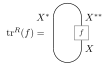
\includegraphics{figures/c17-fig02.svg}


\caption{Left and right traces;
  pivotal isomorphism $\de_X$ and its inverse are not shown.}\label{f:trace}
\end{figure}
Since for a finite tensor category $\End(\one)=\kk$, the traces and dimensions
are elements of $\kk$.

\begin{lemma}\label{l:trace-properties}
  Left and right traces in a pivotal category $\calC$ have the
  following properties \textup{(}stated for $\tr^L$; the
  same holds for $\tr^R$\textup{)}:
  \begin{enumerate}
    \item \textup{(}Cyclicity\textup{)} For any $f\colon X\to Y$ and $g\colon Y\to X$,
      $\tr^L(g\circ f)=\tr^L(f\circ g)$.
    \item \textup{(}Multiplicativity\textup{)} For $f\in \End(X)$, $g\in \End(Y)$,
      $\tr^L(f\otimes g)=\tr^L(f)\,\tr^L(g)$; in particular,
      $\dim^L(X\otimes Y)=\dim^L(X)\,\dim^L(Y)$.
    \item \textup{(}Additivity\textup{)} If $\calC$ is an abelian category, and
      $0\to X'\to X\to X''\to 0$ is a short exact sequence
      and $f\in \End(X)$ preserves $X'$,  inducing $f'\in \End(X')$ and $f''\in
      \End(X'')$, then $\tr^L(f)=\tr^L(f')+\tr^L(f'')$; in particular,
      $\dim^L(X)=\dim^L(X')+\dim^L(X'')$.
    \item \textup{(}Duality\textup{)} $\tr^L(f)=\tr^R(f^*)$, where $f^*\in \End(X^*)$ is the
      dual morphism \textup{(}see \ecref{ec:dual-morphism}\textup{)}; in
      particular,
      $\dim^L(X)=\dim^R(X^*)$.
  \end{enumerate}
\end{lemma}
Proofs, together with a more detailed discussion of pivotal structures and
dimensions, can be found in \cite[Section 4.7]{etingof-fusion}.

\begin{definition}\label{d:spherical}
  A pivotal category $\calC$ is called
  \emph{spherical}\index{category!spherical}
  if for any $X\in \calC$, $f\in \End(X)$ we have
  $$
  \tr^L(f)=\tr^R(f).
  $$
  In this case, we will just use notation $\tr(f)$ for the trace of a morphism
  $f$, and $\dim(X)=\dim^L(X)=\dim^R(X)$ for dimension of an object.
\end{definition}

Note that it is immediate from \leref{l:trace-properties} that in a
spherical category, $\tr(f)=\tr(f^*)$; in particular,
\begin{equation}
 \dim (X)=\dim(X^*).
\end{equation}

\begin{remark}
  All known examples of pivotal categories are spherical. It is an open problem
  if there exist non-spherical pivotal categories.
\end{remark}

\begin{remark}
  Let $\calC$ be a pivotal fusion category. It can be shown that this
  pivotal structure is spherical if and only if $\de^2\colon V\to V^{****}$
  coincides with the canonical isomorphism $V\isoto V^{****}$ mentioned in
  \reref{r:radford}, see \cite[Proposition 3.5.4]{dsps-dualizable}.
\end{remark}

\begin{conjecture}
  Homotopy fixed points of $\SO(3)$ action on $\Tens^\sss$ are spherical fusion
  categories.
\end{conjecture}
Reference: \cite[Conjecture 3.5.10]{dsps-dualizable}.
\include{c18-spherical-src-gerby}
%!TEX root = TQFTbook.tex
%%%%%%%%%%%%%%%%%%%%%%%%%%%%%%
\chapter{Turaev--Viro theory}\label{c:TV}



In this chapter, we define an extended 3-dimensional TQFT called
Turaev--Viro theory. It will be defined as a lattice theory: we will define
$Z(M)$ by choosing a cell decomposition of $M$, writing $Z(M)$ as a state
sum, and then proving that it is independent of the choice of cell
decomposition. In many ways, it is very similar to the definition of
2-dimensional FHK theory in \chref{c:2d-lattice}, but replacing a separable
symmetric Frobenius algebra by a spherical fusion category $\calC$.

This theory was introduced by Turaev and Viro \cite{turaev-viro} in the
special case  when $\calC$ is the category of representations of quantum
group $U_q\su(2)$ with $q$ being a root of unity; in their work, they only
considered the usual (unextended) theory. It was generalized in
\cite{barrett} to arbitrary spherical fusion categories (again, as an
unextended theory); in fact, this was the motivation for introducing the
notion of a spherical fusion category. Extension to 3-2-1 theory was done 
in the series of papers \cite{balsam-kirillov}, 
\cite{balsam-TV2}, \cite{balsam-TV3}. 
Extension down to a point is fairly obvious (we were just too lazy to write 
it down).

Throughout this chapter, $\calC$ is a spherical fusion category over an
algebraically closed field $\kk$ of characteristic zero. We keep all
notation from the previous chapter, in particular denoting by $\OC$ the set
of isomorphism classes of simple objects in $\calC$ and choosing a
representative $X_i$ for each $i\in \OC$. We denote by $E$ the set of oriented
 edges (1-cells) of $M$. A manifold with a choice of PLCW decomposition will be 
 called a combinatorial manifold. Our main reference is \cite{balsam-kirillov}.



%%%%%%%%%%
\section{Turaev--Viro theory in dimensions $0,1$}\label{s:tv-dim01}

Similar to the case of extended 2d TQFT, here we define

$$
Z_\calC(\bullet^+)=\calC, \qquad
Z_\calC(\bullet^-)=\calC^\op
$$

Since the empty zero-dimensional manifold $\emptyset_0$ is the unit under disjoint union,
it must be assigned the unit under Deligne tensor product:

$$
Z_\calC( \emptyset_0)=\vecf
$$

To each unoriented edge $r \in E$, assign an object
\[
E_r = \bigoplus_{i \in \OC}  X_i \boxtimes X_i^* \in \calC_{r'} \boxtimes \calC_{r''}
\]
where $r',r''$ are two possible orientations of $r$. Because of symmetry of $E_r$ ( see \leref{l:spherical-E} ),
 it doesn't matter which orientation is labelled $r'$ or $r''$.

For an oriented 1-manifold $N$ ( possibly with a boundary ) we choose a cell decompostion of it and define
\[
Z_\calC (N) = \dots \boxtimes_\calC \calC \boxtimes_\calC \calC \dots
\]
where a $\calC$ comes from each edge, and a $\boxtimes_\calC$ comes from each internal vertex. ( This is analogous to 
\eqref{e:ZAN-def}, with quotient being achieved by the balanced tensor product. See figure below for a visualization. )

\begin{center}
   	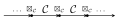
\includegraphics{figures/c19-fig01.svg}
\end{center}

As can be easily shown using \leref{l:bimodule-composition}, this assigns the bimodule category 
$_\calC \calC_\calC$ to an interval ( independent of the cell decomposition )

$$
Z_\calC(I) =  \calC \boxtimes_\calC \boxtimes_\calC \cdots \calC \simeq \calC
$$


This matches with our expectation. Since, the ordinary interval is the identity cobordism of the 
positively oriented point, it should be assigned the identity 1-morphism of $\calC$, which is 
the bimodule category $_\calC \calC_\calC$.

\begin{exercise}
	Show that $Z_\calC ( S^1 ) \simeq \calZ(\calC)$. ( Recall from \thref{t:cat-trace} and \thref{t:category-inv-coinv} 
	that $ \circtensor \calC \simeq  \calC\boxtimes_{\calC^e} \calC \simeq  \calZ(\calC) $. )
\end{exercise}

Since the one-dimensional empty manifold $\emptyset_1$ is unit under disjoint union of one-manifolds, it should 
be assigned $\vecf$ ( as bimodule over $\vecf$ ) by $Z$ functor:

\[
Z_{\calC}(\emptyset_1)=\vecf
\]

We used the subscript $\calC$ in this section just to emphasize that the assignment of data by a Turaev--Viro TQFT 
depends on the choice of $\calC$. We will suppress this subscript in the remaining sections.
%%%%%%%%%%
\section{Turaev--Viro theory in dimension $2$}\label{s:tv-dim2}

We will now consider what kind of data is assigned by $Z$ to a two-dimensional surface $N$. When
 $\partial N = \emptyset$, $Z(N)$ should be a functor from $Z(\emptyset_1)$ to $Z(\emptyset_1)$.

\[ 
Z(N): \vecf \rightarrow \vecf
\]

\begin{exercise}
	Show that $Z(N): \vecf \rightarrow \vecf$ is naturally isomorphic to tensoring with the vector space 
	$$ W_N := Z(N)(\kk).$$ Namely for any vector space $V \in \vecf$, we have $Z(N)(V) \simeq W_M \otimes_\kk V$. 
	Thus we may identify the functor $Z(N)$ with the vector space space $W_N$.
\end{exercise}

This exercise agrees with our expectation that a 3d TQFT should assign a vector space to a closed two-dimensional surface.


More generally, if $\partial N \ne \emptyset$, $Z(N)$ is a functor from the finite abelian category $Z(\ov{\partial  N})$ 
to $\vecf$. Here again we are considering $N$ as a bordism from $\partial N$ to the empty set ( similar to \chref{c:2d-lattice} ).

\[
Z(N): Z(\ov{\partial  N}) \rightarrow \vecf
\]


For a 2-cell $C$ with $n$ edges along it's boundary, this should be a functor:
\[
Z(C):\calC^{\boxtimes n}\to \vecf
\]


Following the general recipe of lattice/state-sum models, 
we will ( soon ) define an invariant of a 3d manifold $M$ by labelling the edges in its cell decomposition by objects of $\calC$.
The orientation and edge labels for 2-cells will be induced from that 3d data. For that purpose, it will be useful to have the 
following defintion.

\begin{definition}
	A labeling of $M$ is a map $l:E \rightarrow \OC $ which assigns to every oriented edge $e$ of $M$ an object $l(e) \in \OC$ 
	such that $l(\ov{e})=l(e)^*$. A labeling is called simple if for every edge, $l(e)$ is simple.
	
	Two labeling $l_1$ and $l_2$ are called equivalent if $l_1(e) \simeq l_2(e)$ for every $e \in E$.

\end{definition}


%%%%%%%%%%%%%%   
\begin{figure}[ht]
	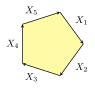
\includegraphics{figures/c19-fig02.svg}
	\hspace{1.5cm} $H(C,l)=\<X_1,X_2,\dots, X_5\>$
	\caption{Defining the state space for a 2-cell}\label{f:state_space1}
\end{figure}
%%%%%%%%%%%%%%   

For a given labeling $l$, we define, for every oriented 2-cell $C$, the state space

\begin{equation}
	H(C,l)=\<l(e_1), l(e_2),\dots, l(e_n)\>,\qquad 
	\del C=e_1\cup e_2\dots\cup e_n
\end{equation}

where the edges $e_1,\dots, e_n$ are taken in the clockwise order on
$\del C$ as shown in \firef{f:state_space1}. The functor $\<\dots\>$ was defined and studied in \seref{s:cat-pairing}. 
In particular, the space $\<c_1,c_2,\dots,c_n\>$ only depends on the cyclic order $c_1,c_2,\cdots,c_n$, and 
not on the starting edge.

For an oriented 2-dimensional combinatorial manifold $N$, we define

\begin{equation}
	H(N, l)= \bigotimes_{C} H(C, l)
\end{equation}

where the product is over all 2-cells. Orientation on each 2-cell $C$ is induced from the orientation of $N$.

\begin{equation}
	H(N,l)=\bigoplus_l H(N,l)
\end{equation}

Finally, we define the state space assigned by the Turaev--Viro theory to $N$ as

\begin{equation}\label{d:TV-surface}
	H(N)= \bigoplus_l H(N,l)
\end{equation}

where the sum is over all simple labelings up to equivalence.

Note that it follows from \eqref{e:dual} that we have canonical isomorphism
\begin{equation}\label{e:H-duality}
	H(\ov{N}) = H(N)^*
\end{equation}

 We have used the notation $H(N)$ for the $Z(N)$ functor in this section to suggest that this data corresponds to 
 the state space associated with the surface $N$. This notation also helps distinguish this assignment from the additional 
 3d-data introduced in the next section.

%%%%%%%%%%
\section{Turaev--Viro theory: full definition}\label{s:tv-full-definition}
We now define the TV invariant of 3-manifolds. Let $M$ be a combinatorial 3-manifold with boundary. We fix a labeling $l$
 of edges of $M$. Then we can assign a vector $Z(F,l) \in H(\partial F, l)$ to  every 3-cell $F$ as follows. Recall that $F$ is an
  inclusion $F:(0,1)^3 \rightarrow M$. The pullback of PLCW decomposition of $M$ gives a PLCW decomposition of 
  $\partial (0,1)^3 \simeq S^2$. Consider the dual graph $\Gamma$ of this decomposition and choose an orientation for every 
  edge of this dual graph ( arbitrarily ) as shown in \firef{f:dual_graph}.

%%%%%%%%%%%%%%
\begin{figure}[ht]
	\centering
	
	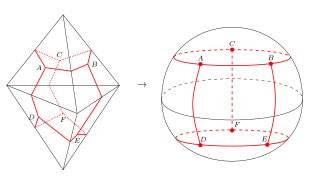
\includegraphics{figures/c19-fig03.svg}
	\caption{The dual graph on the boundary of a 3-cell}\label{f:dual_graph}
\end{figure}
%%%%%%%%%%%%%%

Note that a labeling $l$ of $M$ defines a labeling of edges of this dual graph as shown in figure \firef{f:state_space2}. 
Moreover, choose, for every face $C \in \partial F$, an element $\ph_C \in H(C,l)^*=\<l(e_n)^*,\dots,l(e_1)\>$. Then this 
collection of mrohisms defines a coloring of vertices of $\Gamma$.

By \leref{l:colored-spherical}, we get an invariant $\<\Ga\>_{S^2\setminus\{p\}} \in \kk$, which depends on the choice of
 labeling of edges $l$ and on the choice of morphisms $\ph_C$. We define $Z(F,l) \in \otimes_C H(C,l)$ by

\begin{equation}
	(Z(F,l),\otimes \ph_C)=\<\Ga,l,\{ \ph_C\}\>_{S^2\setminus\{p\}}
\end{equation}

If $F$ is a tetrahedron, then this coincides with the definition in \cite{barrett}; if $\calC$ is the category of representations 
of quantum $\sll_2$, these numbers are the $6j$-symbols.

%%%%%%%%%%%%%%
\begin{figure}[ht]
	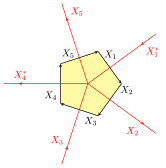
\includegraphics{figures/c19-fig04.svg}\qquad
	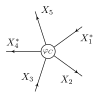
\includegraphics{figures/c19-fig05.svg}
	\qquad $\ph_C \in H(C,l)^*=\<X_5^*,X_4^*, \dots, X_1^*\>$
	\caption{Coloring of the dual graph}\label{f:state_space2}
\end{figure}
%%%%%%%%%%%%%%


We can now give a definition of the TV invariants of combinatorial 3-manifolds.

\begin{definition}\label{d:TV_invariant}
	Let $M$ be a combinatorial 3-manifold with boundary and $\calC$ - a spherical category. Then for any coloring $l$, 
	define a vector
	\[
		Z(M,l) \in H( \partial M,l)
	\]
	by
	\[
	Z(M,l) = \ev\left( \bigotimes_F Z(F,l) \right)
	\]
	where
	\begin{itemize}
		\item $F$ runs over all 3-cells in $M$, each taken with the induced orientation, so that 
		\[
		\bigotimes_F Z(F,l) \in \bigotimes_F H(\partial F,l) = H(\partial M,l) \otimes \bigotimes_c H(c',l) \otimes H(c'',l)
		\]
		\item $c$ runs over all unoriented 2-cells in the interior of $M$; $c'$,$c''$ are the two orientations of such a cell, so 
		that $c'=\ov{c''}$.
		\item $\ev$ is the tensor product over all $c$ of evaluation maps 
		$H(c',l)\otimes H(c'',l)=H(c',l)\otimes H(c',l)^* \rightarrow \kk$
	\end{itemize}
	Finally we define
	\[
	Z(M)= \DD^{-v (M)} \sum_{l} \left(  Z( M,l) \prod_{e} d^{n_e}_{l(e)} \right)
	\]
	where
	\begin{itemize}
		\item the sum is taken over all equivalence classes of simple labelings of $M$,
		\item $e$ runs over the set of all ( unoriented ) edges of $M$,
		\item $\DD$ is the dimension of the category ( defined in \thref{t:drinfeld-dim}), and $v(M)=$number 
		of internal vertices of $M$ + $\frac{1}{2}$(number of vertices on $\partial M$),
		\item $d_{l(e)} $ is the categorical dimension of $l(e)$, and
		$$ n_e = \begin{cases}
			1,\quad e \text{ is an internal edge}\\
			\tfrac{1}{2},\quad e\in \partial M
		\end{cases}
		$$
	\end{itemize}
\end{definition}

In the special case of a triangulated manifold, this coincides with the construction in \cite{barrett}.

\begin{theorem}\label{t:main1}
	If $M$ is a PL manifold without boundary, then the number $Z(M) \in \kk$ defined in \deref{d:TV_invariant} 
	does not depend on the choice of PLCW decomposition of $M$: for any two choices of PLCW decomposition, 
	the resulting invariants are equal.
\end{theorem}

The proofs for this theorem can be found in \cite{balsam-kirillov}.

Moreover, these invariants can be extended to a TQFT. Namely, let $M$ be a combinatorial 3-cobordism between 
two 2-dimensional combinatorial manifolds $N_1$,$N_2$, i.e. a combinatorial manifold $M$ with boundary such
 that $\partial M = \ov{N_1} \sqcup N_2$ ( note that the combinatorial structure on $M$ automatically defines a 
 combinatorial strucutre on $\partial M$). Then $H(\partial M)=H(N_1)^* \otimes H(N_2)=\mathrm{Hom}_\kk ( H(N_1),H(N_2))$, 
 so \deref{d:TV_invariant} defines a linear operator
\[
Z(M): H(N_1) \rightarrow H(N_2)
\]

\begin{theorem}\label{t:main2}
\par\noindent
	\begin{enumerate}
		\item So defined invariant satisfies gluing axiom: if $M$ is a combinatorial 3-manifold with boundary 
		$\partial M=N_0 \cup N \cup \ov{N}$, and $M'$ is the manifold obtained by identifying boundary components 
		$N$,$\ov{N}$ of $\partial M$ with the obvious cell decomposition, then we have
		\[
		Z(M')= \ev_{H(N)} Z(M) = \sum_a (Z(M),\ph_\alpha \otimes \ph^\alpha),
		\]
		where $\ev$ is the evaluation map $H(N)\otimes H(\ov{N}) \rightarrow  \kk $, and $\ph_\alpha \in H(N)$,
		 $\ph^\alpha \in H(\ov{N})$ are dual bases.
		\item If $M$ is a 3-manifold with boundary, and $M'$,$M''$ are two PLCW decompositions of $M$ which 
		agree on the boundary, then $Z(M')=Z(M'') \in H( \partial M')=H(\partial M'')$.
		\item For a combinatorial 2-manifold $N$, define $A_N:H(N) \rightarrow H(N)$ by
		\begin{equation}\label{e:projector}
			A_N=Z(N \times I)
		\end{equation}
		Then $A_N$ is a projector: $A^2_N = A_N$.
		\item For a combinatorial 2-manifold $N$, define the vector space
		\begin{equation}
			Z(N)= \mathrm{Im}(A_N:H(N) \rightarrow H(N))
		\end{equation}
		where $A$ is the projector \eqref{e:projector}. Then the space $\<N\>_{S^2\setminus\{p\}}$ is an invariant of PL 
		manifolds: if $N'$, $N''$ are two different PLCW decompositions of the same PL manifold N, then one has a
		 canonical isomorphism $Z(N') \simeq Z(N'')$.
		\item The assignments $N \mapsto Z(N), M \mapsto Z(M)$ give a functor from the category of PL 3-cobordisms
		 to the category of finite-dimensional vector spaces and thus define a 2+1 dimensional TQFT.
		\end{enumerate}
\end{theorem}

The proof to this theorem can also be found in \cite{balsam-kirillov}.

TODO: The following paragraph should be verified by AK.


 Balsam and Kirillov's state-sum construction  3-2-1 extends the Turaev-Viro 
 theory.  It's natural to ask if they could have fully extended it to a 3-2-1-0 TQFT.  
 In principle, this is doable. But this requires the full complexity of a weak 3 category.
In particular, all the equivalences between ( compositions of ) 1-morphisms 
should hold upto 2-morphisms, and ( compositions of ) 2-morphisms should hold 
 upto 3-morphisms. This leads to a very complicated web of coherence relations. 
 The extension to 0 dimensional manifolds requires a more workable definition of 
 an ($\infty$,3) category.


%%%%%%%%%%
\section{Proof of independence of PLCW decomposition}\label{s:proof}

In this section, we give proofs of \thref{t:main1}, \thref{t:main2},
i.e. prove that TV invariants are independent of the choice of PLCW
decomposition. Before giving the proof, we will enumerate the 
moves that were mentioned in \thref{t:plcw-moves}, in a form more suited 
to this chapter.

\begin{description}
	\item[M1: removing a vertex]
	Let $v$ be a vertex which has a neighborhood whose intersection with 
	the 2-skeleton is homeomorphic to the ``open book'' shown below with
	$k\ge 1$     leaves;    moreover, assume that all leaves in the
	figure are distinct 2-cells and the two
	1-cells  are also  distinct (i.e., not two ends of the same
	edge). Then move M1 removes vertex $v$ and replaces two 1-cells
	adjacent to it with a single 1-cell.
%%%%%%%%%%%%%%   
\begin{figure}[ht]
	\begin{center}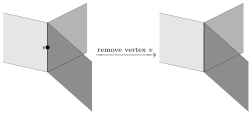
\includegraphics{figures/c19-eqfig02.svg}\end{center}
	\caption{Move M1}\label{f:movef1}
\end{figure}
%%%%%%%%%%%%%%   
	
	\item[M2: removing an edge]
	Let $e$ be a 1-cell which is regular and which is 
	adjacent to exactly two distinct 2-cells $c_1, c_2$ as shown in the
	figure below.  Then the move M2 removes the edge $e$ and replaces
	the cells $c_1,c_2$ with a  single cell $c$. 
%%%%%%%%%%%%%%   
\begin{figure}[ht]
	\begin{center}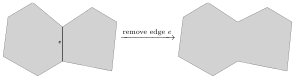
\includegraphics{figures/c19-eqfig03.svg}\end{center}
	\caption{Move M2}\label{f:movef2}
\end{figure}
%%%%%%%%%%%%%%   
	
	\item[M3: removing a 2-cell]
	Let $c$ be a 2-cell which is regular  and which is 
	adjacent to exactly two distinct 3-cells $F_1, F_2$ as shown in the
	figure below.  Then the move M2 removes the 2-cell $c$ and replaces the
	cells $F_1,F_2$ with a single cell $F$.
%%%%%%%%%%%%%%   
\begin{figure}[ht]
	\begin{center}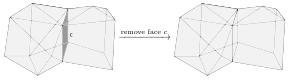
\includegraphics{figures/c19-eqfig04.svg}\end{center}
	\caption{Move M3}\label{f:movef3}
\end{figure}
%%%%%%%%%%%%%%   
	
\end{description}



We will now show that the TV state sum is invariant under M1--M3.

\subsection*{Invariance under M1}
First we consider move M1. Note that by applying M2 and M3, we can
transform an open book  with any number of pages to one with only one page
(see \firef{f:book}). 
\begin{figure}[ht]
	\begin{center}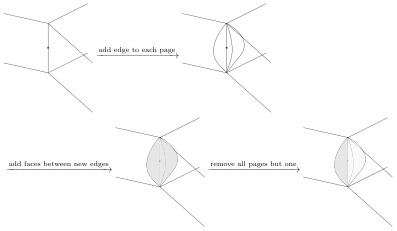
\includegraphics{figures/c19-eqfig05.svg}\end{center}
	\caption{Decomposing an open book into a single page book}\label{f:book}
\end{figure} 


Thus, it suffices to prove invariance under M1 in this
special case. Drawing the dual graph in the vicinity of the vertex,
invariance under M1 is equivalent to the following equality:
\begin{center}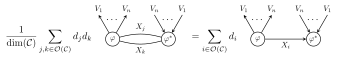
\includegraphics{figures/c19-eqfig06.svg}\end{center}
Note the normalizing factor
$\frac{1}{\mathcal{D}^2}$ which comes from the fact that we are removing a
vertex.

Using semisimplicity of $\C$, it is easy to see that it suffices to show
this equality in the special case when $V=V_1\otimes \dots \otimes V_n$ is
simple:
\begin{center}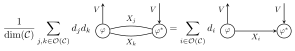
\includegraphics{figures/c19-eqfig07.svg}\end{center}

By \leref{l:pairing}, the right-hand side is equal to $\coev_V\colon \one
\to V\otimes V^*$. Since $\Hom(\one, V\otimes V^*)$ is one-dimensional,
the left-hand side is also a multiple of $\coev_V$. Composing it with the
evaluation morphism  $\ev_V$, we get
\begin{align*}
	&\frac{1}{\DD}\sum_{j,k}d_jd_kN_{1}^{Vjk} =
	\frac{1}{\DD}\sum_{j,k}N_{k^*}^{Vj}d_kd_j\\
	&\quad=\frac{1}{\DD}\sum_{j}\Bigl(\sum_{k}N_{k^*}^{Vj}d_k\Bigr)d_j=
	\frac{1}{\DD}\sum_{j}(d_{V}d_j)d_j=d_V,
\end{align*}
which proves that the left-hand side is equal to $\coev_V$.






\subsection*{Invariance under M2}
The invariance under M2 is seen as follows. By definition, the edge being
removed is incident to exactly two faces $c_1, c_2$. Each face bounds the
same two 3-cells $F_1, F_2$. In  \firef{f:move2}, we draw the dual graphs.
In each of the summands we have two graphs corresponding to cells $F_1,
F_2$, separated by a dot.  The equality follows
immediately from the fact that if $\ph_\al,\ph^\al$ and $\psi_\be,\psi^\be$ 
are dual bases, then so are $\ph_\al\ccc{X_i}\psi_\be$, $\psi^\be\ccc{X_i^*}\ph^\al$ 
(cf. \coref{c:composition2}). 
\begin{figure}[ht]
	\begin{center}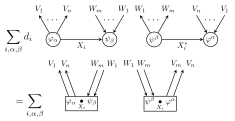
\includegraphics{figures/c19-eqfig08.svg}\end{center}
	\caption{}\label{f:move2}
\end{figure}

\subsection*{Invariance under M3}
Finally, we consider M3. In this case the invaraince immediately follows
from \leref{l:pairing2}, whith  two subgraphs corresponding to two 3-cells
separated by the 2-cell being removed.


%%%%%%%%%%%%%%%%%%%%%%%%%%%%%%%%
\section{String-net model}\label{s:stringnet}


In this section we look at a physics model which, in a certain limit, is described 
by Turaev--Viro TQFT. This model was introduced  by Levin-Wen \cite{levin-wen}, 
and is known as the string-net model. Roughly speaking, a state in this model
consists of highly fluctuating ``string-nets'' on a closed surface $N$, which are  
colored graphs on $N$ modulo some local relations. The allowed graphs
on these string-nets alongwith the local relations encode the data of a spherical
fusion category $\calC$.  We will here outline the correspondence between the string-net
 model and Turaev--Viro TQFT. Formal details, including the most
general proof for this correspondence can be found in \cite{kirillov-stringnet}. 
We also use this section to make some general comments about how TQFTs are viewed
in relation to gapped quantum systems in physics.


Using the \deref{d:colored-graph} of a colored graph, we denote
  $$
\mathrm{Graph}(N)=\text{set of all $\calC$-colored graphs in $N$ }
$$

We can also consider formal linear combinations of colored graphs. 
We denote
 $$
\mathrm{VGraph}(N)=\text{formal linear combinations of graphs }\Gamma \in \mathrm{Graph}(N) 
$$

\begin{definition}\label{d:null-graph}
	Let $D \in N$ be an embedded disk. We define a null graph $\boldsymbol{\Gamma} = c_1 \Gamma_1 + \cdots + c_n \Gamma_n 
	\in \mathrm{VGraph}(N)$ to be a linear combination of clolored graphs in $N$ such that:
	\begin{enumerate}
		\item $\Gamma$ is transerversal to $\del D$ (i.e., no vertices of $\Gamma_i$ are on the boundary 
		of $D$ and edges of each $\Gamma_i$ meet $\del D$ transversally).
		\item  All $\Gamma_i$ coincide outside of $D$.
		\item $\< \boldsymbol{\Gamma} \>_D = \sum c_i \< \Gamma_i \cap D \>_D =0$, where 
		$ \< \Gamma_i \cap D \>_D$ is the expectation value defined by \thref{t:evaluation-disk}.
	\end{enumerate}
\end{definition}

The local relations ( adapted to our discussion ) are given in \firef{f:local_rels1}. More physics
oriented illustrations of local relations can be found in the original paper \cite{levin-wen}.

\begin{definition}
	Let $N$ be an oriented closed surface. The string-net space $H^{string}(N)$ is the quotient space
	\[
		H^{string}(N) = \mathrm{VGraph}(N)/\mathrm{VGraph}_0(N)
	\]
	where $\mathrm{VGraph}_0(N)$ is the subspace spanned by null graphs ( for all possible embedded 
	disks $D \in N$).
\end{definition}

The correspondence between Turaev--Viro TQFT and string-net models is the 
following theorem.

\begin{theorem}\label{t:tv-equals-stringnet}
	Let $N$ be a closed oriented surface. Then one has a canonical isomorphism
	\[
		H^{string}(N) \simeq Z(N),
	\]
	where the Turaev--Viro functor $Z(N)$ was defined in \deref{d:TV-surface}.
\end{theorem}

In fact, the correspondence can also be extended to surfaces with boundaries. 
In the languge of string-nets, surfaces with boundaries describe excited states. 
A surface with boundaries can be obtained from an oriented closed surface
by removing some discs. These would-be-discs are said to host quasiparticles 
or anyons. Different possible quasiparticles in the string-net model are given 
by the simple objects of $\calZ(\calC)$ --- the Drinfeld center of $\calC$. 
The proof and the precise statement can again be found in \cite{kirillov-stringnet}.
Heuristically, a quasiparticle must admit a consistent rule for moving any string labeled
by an object of $\calC$ past it. Such a rule is precisely the half-braiding, and its
compatibility with the tensor product of $\calC$ is the hexagon axiom 
(compare \deref{d:drinfeld-center}).

The string-net model provides a microscopic Hamiltonian ( on a lattice ) for the given
spherical fusion category $\calC$. The 
Hamiltonian operator is engineered such the its
ground states necessarily obey the local relations. The states invariant under
the local moves are constructed by taking superposition of all graphs
related through local moves. In this sense, the ground states in the string-net model are
described as fluctuating string-nets, or condensed string-nets. Note that the actual 
string-net model has excited states too, but their energy gap relative to the
ground state(s) is large enough that they can be ignored while working with low
energy processes. We say that the string-net model is ``gapped'', and the model
flows ( under renormalization ) to a TQFT.
This is a recurring theme in the physics literature: the low energy
limit of a gapped quantum system is described by a TQFT. After enough coarse-graining,
any observable should be insensitive to local relations. The microscopic details,
including the choice of lattice, get washed out when the theory reaches the low energy 
fixed point of the renormalization group flow. This was partly the motivation used by Levin-Wen 
to come up with the string-net model.



%%%%%%%%%%
\section{Example: Dijkgraaf--Witten in 3 dimensions}\label{s:tv-dw3}
In this section we look at an explicit example. We consider $\calC = \vect_G$, which was defined in \exref{x:vecg}. 
We choose $G$ to be some finite group, and the underlying field is $\C$ . We shall see that the Turaev--Viro theory 
associated to this $\calC$ is the Dijkgraaf--Witten theory in 3 dimensions. We refer the reader to 
\cite[Theorem 4.2]{petit} for a proof.

The simple objects in $\calC$ are complex one-dimensional spaces graded with an element $g \in G$. We 
denote such a simple object as $\C_g$. A simple labeling $l$ will assign a group element $g_e$ to every oriented edge.
To a $n$-side face whose boundary labels are ${g_1},\dots,{g_n}$ ( in cylic order ), the functor $Z$ assigns
\begin{align}\label{e:flatness}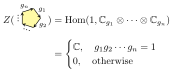
\includegraphics{figures/c19-eqfig01.svg}\end{align}

So the state space $H(N)$ for a 2-dimensional manifold $N$ is the space of flat $G$-connections. The categorical 
dimension of each edge is $1$ for $\calC$ . This gives $\mathrm{dim}(\calC)= |G|$. The projector $A_N$ thus 
takes the form
\[
A_N = \frac{1}{|G|^{v(N \times I)}}   \sum_{l_{\mathrm{flat}} } \left(  Z( N \times I ,l_{\mathrm{flat}}) \right).
\]

For a state $|a \> \in H(N)$, the sum over all flat gauge configurations $l_\mathrm{flat}$ on $N \times I$ gives a sum
 over all states $| h.a \>$, that are connected to $|a\>$ via some some element $h$ of the gauge group $G^{v(N)}$.
  As shown in \firef{f:flat-guage-configuration}, for each labeling $|a \>$ of $N$, an element $h \in G^{v(N)}$ leads 
  to another labeling $| b \>$ that is related to $| a \>$ by a gauge transformation. So the action of averaging 
  over $G^{v(N)}$ projects the states in $H(N)$ to $G^{v(N)}$-invariant states.  Thus $Z(N)$ is precisely the vector 
  space spanned by gauge equivalence classes of $G$-connections on $N$.


\begin{figure}[ht]
	\centering
	   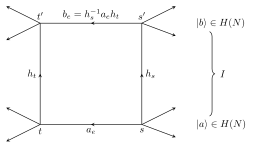
\includegraphics{figures/c19-fig06.svg}
\caption{A sample configuration appearing in the $\sum_{l_{\mathrm{flat}}} Z(N \times I , l_{\mathrm{flat}} )$. 
	Bottom of the diagram shows a portion of configuration $| a \>$ assigned to a closed 2-manifold $N$. $|a\>$ 
	assigns an $a_e \in G$ to each edge $e$, but we are showing only the edge $e$ between $s$ and $t$ here. 
	We label the vertical edges by elements $h_v$ of $G^{v(N)}$ for each $v \in v(N)$. 
	The flatness condition imposes that the configuration $|b\>$ on the other end of interval $I$ is a 
	gauge transformation of $|a\>$, i.e. $|b\>=|h.a\>$.}
\label{f:flat-guage-configuration}
\end{figure}

Similarly, for a 3-dimensional manifold $M$, we have
\begin{equation}\label{e:untwisted-DW}
	Z(M) = \frac{1}{|G|^{v(M)}} (\text{number of flat colorings})
\end{equation}
For a closed manifold, this counts isomorphism classes of principal G-bundles on $M$ ( with the appropriate
 weight that was described in \seref{s:DW-definition} ). This is same as the untwisted Dijkgraaf--Witten theory
  in 3 dimensions.


We can generalize this example by considering $\calC = \vect_G^\omega$ as was defined in \exref{x:vecg-twisted}. 
The choice of the 3-cocycle $\omega$ does not change the flatness condition coming from \eqref{e:flatness}. 
But the contribution $\<\Ga,l,\{ \ph_C\}\>_{S^2\setminus\{p\}}$ 
 coming from each oriented 3-cell $[0,1,2,3]$ now gets modified by $\omega(g_{01},g_{12},g_{23})$ or 
 $\omega(g_{01},g_{12},g_{23})^{-1}$ depending on its orientation with respect to the manifold $M$. Note that a 3-cell 
 has only 3 independent edge labels due to flatness condition. The Turaev--Viro partition function then takes the form
\begin{equation}\label{e:twisted-DW}
Z(M) = \frac{1}{|G|^{v(M)}} \sum_{l_\mathrm{flat}} \prod_{c \in \mathrm{3-cells}} \omega(g_1(c),g_2(c),g_3(c))^{\sigma(c)}
\end{equation}
where $\sigma(c) = \pm 1 $ depending on the relative orientation of the 3-cell $c$ with respect to $M$, and 
$g_1(c),g_2(c),g_3(c)$ are group elements labelling the edges of $c$ in a certain order. This turns out to be 
the state sum defintion of the twisted 3-dimensional Dijkgraaf--Witten theory ( compare \eqref{e:DW-integral} ). The
 untwisted theory \eqref{e:untwisted-DW} can be obtained from \eqref{e:twisted-DW} by settings $\omega=1$.


It is worth commenting here that Turaev--Viro TQFTs based on $\vect_G$, with $G$ a finite abelian group,
 are also very interesting from the physics perspective. These TQFTs describe the topological phases realized 
 by quantum double models. In particular, the simple objects in $Z(S^1)$ correspond to anyons in a 
 quantum double model, which have potential applications in topological quantum computing. A famous example
  is Kitaev's toric code \cite{kitaev}, which is based on $G=\Z_2$.


%%%%%%%%%%%%%%%%%%%%
\section{Comparison with cobordism hypothesis}\label{auto:c19-TV-comparison-with-cobordism-hypothesis}
FIXME: discuss relation of this to the construction fo extended 3d TQFT via cobordims hypothesis, see Chapter 17. 

\part{Chern--Simons and Crane--Yetter theories}\label{p:chern-simons}
\include{c20-321-src-gerby}
\end{document}
